% Options for packages loaded elsewhere
\PassOptionsToPackage{unicode}{hyperref}
\PassOptionsToPackage{hyphens}{url}
\PassOptionsToPackage{dvipsnames,svgnames,x11names}{xcolor}
%
\documentclass[
  a4paper,11pt,twoside,onecolumn,openright,final,oldfontcommands]{memoir}
\usepackage{amsmath,amssymb}
\usepackage{lmodern}
\usepackage{iftex}
\ifPDFTeX
  \usepackage[T1]{fontenc}
  \usepackage[utf8]{inputenc}
  \usepackage{textcomp} % provide euro and other symbols
\else % if luatex or xetex
  \usepackage{unicode-math}
  \defaultfontfeatures{Scale=MatchLowercase}
  \defaultfontfeatures[\rmfamily]{Ligatures=TeX,Scale=1}
\fi
% Use upquote if available, for straight quotes in verbatim environments
\IfFileExists{upquote.sty}{\usepackage{upquote}}{}
\IfFileExists{microtype.sty}{% use microtype if available
  \usepackage[]{microtype}
  \UseMicrotypeSet[protrusion]{basicmath} % disable protrusion for tt fonts
}{}
\makeatletter
\@ifundefined{KOMAClassName}{% if non-KOMA class
  \IfFileExists{parskip.sty}{%
    \usepackage{parskip}
  }{% else
    \setlength{\parindent}{0pt}
    \setlength{\parskip}{6pt plus 2pt minus 1pt}}
}{% if KOMA class
  \KOMAoptions{parskip=half}}
\makeatother
\usepackage{xcolor}
\usepackage{color}
\usepackage{fancyvrb}
\newcommand{\VerbBar}{|}
\newcommand{\VERB}{\Verb[commandchars=\\\{\}]}
\DefineVerbatimEnvironment{Highlighting}{Verbatim}{commandchars=\\\{\}}
% Add ',fontsize=\small' for more characters per line
\usepackage{framed}
\definecolor{shadecolor}{RGB}{248,248,248}
\newenvironment{Shaded}{\begin{snugshade}}{\end{snugshade}}
\newcommand{\AlertTok}[1]{\textcolor[rgb]{0.94,0.16,0.16}{#1}}
\newcommand{\AnnotationTok}[1]{\textcolor[rgb]{0.56,0.35,0.01}{\textbf{\textit{#1}}}}
\newcommand{\AttributeTok}[1]{\textcolor[rgb]{0.77,0.63,0.00}{#1}}
\newcommand{\BaseNTok}[1]{\textcolor[rgb]{0.00,0.00,0.81}{#1}}
\newcommand{\BuiltInTok}[1]{#1}
\newcommand{\CharTok}[1]{\textcolor[rgb]{0.31,0.60,0.02}{#1}}
\newcommand{\CommentTok}[1]{\textcolor[rgb]{0.56,0.35,0.01}{\textit{#1}}}
\newcommand{\CommentVarTok}[1]{\textcolor[rgb]{0.56,0.35,0.01}{\textbf{\textit{#1}}}}
\newcommand{\ConstantTok}[1]{\textcolor[rgb]{0.00,0.00,0.00}{#1}}
\newcommand{\ControlFlowTok}[1]{\textcolor[rgb]{0.13,0.29,0.53}{\textbf{#1}}}
\newcommand{\DataTypeTok}[1]{\textcolor[rgb]{0.13,0.29,0.53}{#1}}
\newcommand{\DecValTok}[1]{\textcolor[rgb]{0.00,0.00,0.81}{#1}}
\newcommand{\DocumentationTok}[1]{\textcolor[rgb]{0.56,0.35,0.01}{\textbf{\textit{#1}}}}
\newcommand{\ErrorTok}[1]{\textcolor[rgb]{0.64,0.00,0.00}{\textbf{#1}}}
\newcommand{\ExtensionTok}[1]{#1}
\newcommand{\FloatTok}[1]{\textcolor[rgb]{0.00,0.00,0.81}{#1}}
\newcommand{\FunctionTok}[1]{\textcolor[rgb]{0.00,0.00,0.00}{#1}}
\newcommand{\ImportTok}[1]{#1}
\newcommand{\InformationTok}[1]{\textcolor[rgb]{0.56,0.35,0.01}{\textbf{\textit{#1}}}}
\newcommand{\KeywordTok}[1]{\textcolor[rgb]{0.13,0.29,0.53}{\textbf{#1}}}
\newcommand{\NormalTok}[1]{#1}
\newcommand{\OperatorTok}[1]{\textcolor[rgb]{0.81,0.36,0.00}{\textbf{#1}}}
\newcommand{\OtherTok}[1]{\textcolor[rgb]{0.56,0.35,0.01}{#1}}
\newcommand{\PreprocessorTok}[1]{\textcolor[rgb]{0.56,0.35,0.01}{\textit{#1}}}
\newcommand{\RegionMarkerTok}[1]{#1}
\newcommand{\SpecialCharTok}[1]{\textcolor[rgb]{0.00,0.00,0.00}{#1}}
\newcommand{\SpecialStringTok}[1]{\textcolor[rgb]{0.31,0.60,0.02}{#1}}
\newcommand{\StringTok}[1]{\textcolor[rgb]{0.31,0.60,0.02}{#1}}
\newcommand{\VariableTok}[1]{\textcolor[rgb]{0.00,0.00,0.00}{#1}}
\newcommand{\VerbatimStringTok}[1]{\textcolor[rgb]{0.31,0.60,0.02}{#1}}
\newcommand{\WarningTok}[1]{\textcolor[rgb]{0.56,0.35,0.01}{\textbf{\textit{#1}}}}
\usepackage{longtable,booktabs,array}
\usepackage{calc} % for calculating minipage widths
% Correct order of tables after \paragraph or \subparagraph
\usepackage{etoolbox}
\makeatletter
\patchcmd\longtable{\par}{\if@noskipsec\mbox{}\fi\par}{}{}
\makeatother
% Allow footnotes in longtable head/foot
\IfFileExists{footnotehyper.sty}{\usepackage{footnotehyper}}{\usepackage{footnote}}
\makesavenoteenv{longtable}
\usepackage{graphicx}
\makeatletter
\def\maxwidth{\ifdim\Gin@nat@width>\linewidth\linewidth\else\Gin@nat@width\fi}
\def\maxheight{\ifdim\Gin@nat@height>\textheight\textheight\else\Gin@nat@height\fi}
\makeatother
% Scale images if necessary, so that they will not overflow the page
% margins by default, and it is still possible to overwrite the defaults
% using explicit options in \includegraphics[width, height, ...]{}
\setkeys{Gin}{width=\maxwidth,height=\maxheight,keepaspectratio}
% Set default figure placement to htbp
\makeatletter
\def\fps@figure{htbp}
\makeatother
\usepackage[normalem]{ulem}
\setlength{\emergencystretch}{3em} % prevent overfull lines
\providecommand{\tightlist}{%
  \setlength{\itemsep}{0pt}\setlength{\parskip}{0pt}}
\setcounter{secnumdepth}{5}
\newlength{\cslhangindent}
\setlength{\cslhangindent}{1.5em}
\newlength{\csllabelwidth}
\setlength{\csllabelwidth}{3em}
\newlength{\cslentryspacingunit} % times entry-spacing
\setlength{\cslentryspacingunit}{\parskip}
\newenvironment{CSLReferences}[2] % #1 hanging-ident, #2 entry spacing
 {% don't indent paragraphs
  \setlength{\parindent}{0pt}
  % turn on hanging indent if param 1 is 1
  \ifodd #1
  \let\oldpar\par
  \def\par{\hangindent=\cslhangindent\oldpar}
  \fi
  % set entry spacing
  \setlength{\parskip}{#2\cslentryspacingunit}
 }%
 {}
\usepackage{calc}
\newcommand{\CSLBlock}[1]{#1\hfill\break}
\newcommand{\CSLLeftMargin}[1]{\parbox[t]{\csllabelwidth}{#1}}
\newcommand{\CSLRightInline}[1]{\parbox[t]{\linewidth - \csllabelwidth}{#1}\break}
\newcommand{\CSLIndent}[1]{\hspace{\cslhangindent}#1}
%%%%%%%%%%%%%%%%%%%%%%%%%%%%%%%%%%%%%%%%%%%%%%%%%%%%%%%
% Loading packages
%%%%%%%%%%%%%%%%%%%%%%%%%%%%%%%%%%%%%%%%%%%%%%%%%%

%\usepackage[tikz]{mdframed}
\usepackage{tikz}
\usepackage{mdframed}
\mdfsetup{skipabove=1em,skipbelow=1em}
\newmdenv[backgroundcolor=kcblue]{note}

% \usepackage{babel} % throws an error...
% \usepackage{amsmath,amssymb,amsthm,enumitem} % for equations

\usepackage{polyglossia}
\setmainlanguage{french}

\usepackage{fontspec}
\setmainfont{Heuristica}

%%%%%%%%%%%%%%%%%%%%%%%%%%%%%%%%%%%%%%%%%%%%%
% title page color
%%%%%%%%%%%%%%%%%%%%%%%%%%%%%%%%%%%%%%%%%

% \usepackage[pagecolor=none]{pagecolor}
% \usepackage{afterpage}
% \usepackage{xcolor}

% \setmainfont{FreeSerif} % for unicode emojis
% fonts that support a symbol:
% http://www.fileformat.info/info/unicode/char/1f64c/fontsupport.htm

%%%%%%%%%%%%%%%%%%%%%%%%%%%%%%%%%%%%%%%%%%%%%
% links and citations colors
%%%%%%%%%%%%%%%%%%%%%%%%%%%%%%%%%%%%%%%%

\definecolor{blogblue}{RGB}{0, 51, 102}

\usepackage{hyperref}

\hypersetup{
    colorlinks = true,
    linkcolor = blogblue,
    filecolor = blogblue,
    urlcolor = blogblue,
    citecolor = blogblue
}

%%%%%%%%%%%%%%%%%%%%%%%%
% Remove default title %
% https://stackoverflow.com/questions/45963505/coverpage-and-copyright-notice-before-title-in-r-bookdown
%%%%%%%%%%%%%%%%%%%%%%%%

%\usepackage[a4paper]{./latex/cover_page} % specifies the path to the cover page template
%\let\oldmaketitle\maketitle
%\AtBeginDocument{\let\maketitle\relax}

%%%%%%%%%%%%%%%%%%%%%%%%%%%%%%%%%%%%%%%%%%%%%%%%%%%%%%%%%%%%%
% Format of the page (block, header, margins, etc.)         %
% https://texdoc.net/texmf-dist/doc/latex/memoir/memman.pdf %
%%%%%%%%%%%%%%%%%%%%%%%%%%%%%%%%%%%%%%%%%%%%%%%%%%%%%%%%%%%%%

% Sets the "real" paper size (already set by a4paper class option)
% \setstocksize{11in}{8.5in}

% Trimmed paper size (trimmed on the left and right)
% \settrimmedsize{11in}{8.5in}{*}

% Sets the \headheight and \footskip parameters (respectively)
% \setheadfoot{\onelineskip}{2\onelineskip}

% Sets space between header and block
% \setheaderspaces{*}{2\onelineskip}{*}

% Spine and trim page margins from main typeblock (left and right margins if oneside)
\setlrmarginsandblock{25mm}{25mm}{*}

% Top and bottom page margins from main typeblock
\setulmarginsandblock{25mm}{*}{1}

% Applies and enforces the layout
\checkandfixthelayout

% Ensures single spacing between sentences
\frenchspacing

% eliminating paragraph indentation and using extra inter- paragraph space
\setlength{\parindent}{0pt}
\nonzeroparskip

%%%%%%%%%%%%%%%%%%%%%%%%
% Formatting
%%%%%%%%%%%%%%%%%%%%

\usepackage{calc} % simple arithmetics in latex commands
\usepackage{soul} % hyphenation for letterspacing, underlining, etc.

\makeatletter
\newlength\dlf@normtxtw
\setlength\dlf@normtxtw{\textwidth}
\newsavebox{\feline@chapter}
\newcommand\feline@chapter@marker[1][4cm]{%
	\sbox\feline@chapter{%
		\resizebox{!}{#1}{\fboxsep=1pt%
			\colorbox{gray}{\color{white}\thechapter}%
		}}%
		\rotatebox{90}{%
			\resizebox{%
				\heightof{\usebox{\feline@chapter}}+\depthof{\usebox{\feline@chapter}}}%
			{!}{\scshape\so\@chapapp}}\quad%
		\raisebox{\depthof{\usebox{\feline@chapter}}}{\usebox{\feline@chapter}}%
}

\newcommand\feline@chm[1][4cm]{%
	\sbox\feline@chapter{\feline@chapter@marker[#1]}%
	\makebox[0pt][c]{% aka \rlap
		\makebox[1cm][r]{\usebox\feline@chapter}%
	}}

\makechapterstyle{daleifmodif}{
\renewcommand\chapnamefont{\normalfont\Large\scshape\raggedleft\so}
\renewcommand\chaptitlefont{\normalfont\Large\bfseries\scshape}
\renewcommand\chapternamenum{} \renewcommand\printchaptername{}
\renewcommand\printchapternum{\null\hfill\feline@chm[2.5cm]\par}
\renewcommand\afterchapternum{\par\vskip\midchapskip}
\renewcommand\printchaptertitle[1]{\color{gray}\chaptitlefont\raggedleft
  \renewcommand\chaptername{Chapter}
  ##1\par}
}

\makeatother
\chapterstyle{daleifmodif}

% The pages should be numbered consecutively at the bottom centre of the page
\makepagestyle{myvf}
\makeoddfoot{myvf}{}{\thepage}{}
\makeevenfoot{myvf}{}{\thepage}{}
\makeheadrule{myvf}{\textwidth}{\normalrulethickness}
\makeevenhead{myvf}{\small\textsc{\leftmark}}{}{}
\makeoddhead{myvf}{}{}{\small\textsc{\rightmark}}
\pagestyle{myvf}

%%%%%%%%%%%%%%%%%%%%%%%%
% Insert an empty page %
%%%%%%%%%%%%%%%%%%%%%%%%

\usepackage{afterpage} % executes command after the next page break

\newcommand\blankpage{%
    \null
    \thispagestyle{empty}%
    % \addtocounter{page}{-1}% % uncomment to increase page counter
    \newpage
    }

\newcommand{\clearemptydoublepage}{\newpage{\thispagestyle{empty}\cleardoublepage}}

%%%%%%%%%%%%%%%%%%%%%%%%%%%%%%%%%%%%%%%%%%%%%%%%%%%%%%%%%%%%%%%%%%%%%%%%%%%%%%%%%%%%
% boxes and cie
% from https://github.com/mca91/EconometricsWithR/blob/master/preamble.tex
%%%%%%%%%%%%%%%%%%%%%%%%%%%%%%%%%%%%%%%%%%%%%%%%%%%%%%%%%%%%%%%%%%%%%%%%%%%%%%%%

\usepackage{tcolorbox}

\definecolor{kcblue}{HTML}{D7DDEF}
\definecolor{kcdarkblue}{HTML}{2B4E70}

\newenvironment{rmdknit}
    {\begin{center}
    \begin{tabular}{|p{0.9\textwidth}|}
    \hline\\
    }
    {
    \\\\\hline
    \end{tabular}
    \end{center}
    }

\newenvironment{rmdnote}
    {\begin{center}
    \begin{tabular}{|p{0.9\textwidth}|}
    \hline\\
    }
    {
    \\\\\hline
    \end{tabular}
    \end{center}
    }

\newtcolorbox[auto counter, number within=section]{keyconcepts}[2][]{%
colback=kcblue,colframe=kcdarkblue,fonttitle=\bfseries, title=Concept essentiel~#2, after title={\newline #1}, beforeafter skip=15pt}

%%%%%%%%%%%%%%%%%%%%%%%%%%%%%%%%%%%%%%%%%%%%%%%%%%%%%%%%%%%%
% create classes for theorem and definitions
%%%%%%%%%%%%%%%%%%%%%%%%%%%%%%%%%%%%%%%%%%%%%%%%%%

%\usepackage{amsthm}
%\newtheorem{theorem}{Théorème}
%\newtheorem{definition}{Définition}

%%%%%%%%%%%%%%%%%%%%%%%%%%%%%%%%%%%%%%%%%%%%%%%%%%%%
% Command used in the manual list of abbreviations %
%%%%%%%%%%%%%%%%%%%%%%%%%%%%%%%%%%%%%%%%%%%%%%%%%%%%

\newcommand\nomenclature[2]{#1 & #2 \\}

%%%%%%%%%%%%%%%%%%
% Epigraph style %
%%%%%%%%%%%%%%%%%%

\usepackage{epigraph} % provides commands to assist in the typesetting of a single epigraph

\setlength\epigraphwidth{1\textwidth}
\setlength\epigraphrule{0pt} % no line between
\setlength\beforeepigraphskip{1\baselineskip} % space before and after epigraph
\setlength\afterepigraphskip{2\baselineskip}
\renewcommand*{\textflush}{flushright}
\renewcommand*{\epigraphsize}{\normalsize\itshape}

%%%%%%%%%%%%%%%%%%%%%%%%%%%%%%%%%%%%%%%%%%%%%%
% tables
%%%%%%%%%%%%%%%%%%%%%%%%%%%%%%%%%%%%%%%%%%%%%

% \usepackage{booktabs}
% \usepackage{longtable}
% \usepackage{array}
% \usepackage{multirow}
% \usepackage{wrapfig}
% \usepackage{float}
% \usepackage{colortbl}
% \usepackage{pdflscape}
% \usepackage{tabu}
\usepackage{threeparttable}
\usepackage{threeparttablex}
% \usepackage[normalem]{ulem}
% \usepackage{makecell}

%%%%%%%%%%%%%%%%%%%%%%%%%%%%%%%%%%%%%%%%%%%%%%%%%%%%%%%%%%%%
% changing figures and tables names
% https://tex.stackexchange.com/questions/17489/change-caption-name-of-figures
%%%%%%%%%%%%%%%%%%%%%%%%%%%%%%%%%%%%%%%%%%%%%%%%%%%%%%%%%%%%

\usepackage[figurename = Figure]{caption}
\usepackage[tablename = Tableau]{caption}
\ifLuaTeX
  \usepackage{selnolig}  % disable illegal ligatures
\fi
\IfFileExists{bookmark.sty}{\usepackage{bookmark}}{\usepackage{hyperref}}
\IfFileExists{xurl.sty}{\usepackage{xurl}}{} % add URL line breaks if available
\urlstyle{same} % disable monospaced font for URLs
\hypersetup{
  pdftitle={Notes de cours - Introduction à la modélisation statistique bayésienne},
  pdfauthor={Ladislas Nalborczyk},
  colorlinks=true,
  linkcolor={Maroon},
  filecolor={Maroon},
  citecolor={Blue},
  urlcolor={Blue},
  pdfcreator={LaTeX via pandoc}}

\title{Notes de cours - Introduction à la modélisation statistique bayésienne}
\usepackage{etoolbox}
\makeatletter
\providecommand{\subtitle}[1]{% add subtitle to \maketitle
  \apptocmd{\@title}{\par {\large #1 \par}}{}{}
}
\makeatother
\subtitle{Un cours en R avec brms}
\author{Ladislas Nalborczyk}
\date{Dernière mise à jour : 14-10-2022}

\usepackage{amsthm}
\newtheorem{theorem}{Théorème}[chapter]
\newtheorem{lemma}{Lemme}[chapter]
\newtheorem{corollary}{Corollaire}[chapter]
\newtheorem{proposition}{Proposition}[chapter]
\newtheorem{conjecture}{Conjecture}[chapter]
\theoremstyle{definition}
\newtheorem{definition}{Définition}[chapter]
\theoremstyle{definition}
\newtheorem{example}{Exemple}[chapter]
\theoremstyle{definition}
\newtheorem{exercise}{Exercice}[chapter]
\theoremstyle{definition}
\newtheorem{hypothesis}{Hypothesis}[chapter]
\theoremstyle{remark}
\newtheorem*{remark}{Remarque }
\newtheorem*{solution}{Solution}
\begin{document}
\maketitle

%%%%%%%%%%%%%%%%%%%%%%%%%%%%%%%%%%%%
% title page layout
%%%%%%%%%%%%%%%%%%%%%%%%%%%%%%%%

\thispagestyle{empty}

% background color
% \newpagecolor{blogblue}\afterpage{\restorepagecolor}

\begin{center} % horizontal centering

  \includegraphics[width=0.8\textwidth]{figures/cover_distributions.png}

\end{center}

\newpage
\blankpage % leaves a blank page between title and TOC

\OnehalfSpacing % increasing line spacing to 1.5 (but leaving footnote to 1)

\pagenumbering{roman} % start page numbering (roman style)

{
\hypersetup{linkcolor=}
\setcounter{tocdepth}{2}
\tableofcontents
}
\hypertarget{pruxe9face}{%
\chapter*{Préface}\label{pruxe9face}}
\addcontentsline{toc}{chapter}{Préface}

\pagenumbering{arabic}

Ce document regroupe les notes de l'édition 2022 de la formation doctorale ``Introduction à la modélisation statistique bayésienne'', co-organisée par le collège des écoles doctorales de l'Université Grenoble Alpes et la Maison de la Modélisation et de la Simulation, Nanoscience, et Environnement (MaiMoSiNE).

Ces notes de cours sont organisées en suivant la structure du cours, avec un chapitre par cours, résumant les notions essentielles et donnant quelques éléments de contexte et/ou techniques supplémentaires, pour les plus curieux.

Vous pouvez télécharger la version PDF de ce document en cliquant sur l'icône PDF dans la barre d'outils figurant tout en haut de la version en ligne de ce document. Les slides, données, et codes utilisés sont également disponibles sur le répertoire Github du cours : \url{https://github.com/lnalborczyk/IMSB2022}.

Le contenu de ce livret est largement inspiré du livre \emph{Statistical rethinking} (\protect\hyperlink{ref-mcelreath_statistical_2016}{McElreath, 2016b}, \protect\hyperlink{ref-mcelreath_statistical_2020}{2020}) et des cours partagés librement en ligne par l'auteur. Par ailleurs, le format (HTML) du livret est en partie repris du livre \emph{Introduction to Econometrics with R} (\protect\hyperlink{ref-hanck_introduction_2018}{Hanck et al., 2018}), disponible \href{https://bookdown.org/machar1991/ITER/}{en ligne}.

Enfin, ce document est diffusé sous une licence \emph{Creative Commons Attribution - Pas d'utilisation commerciale - Partage dans les mêmes conditions} (\url{https://creativecommons.org/licenses/by-nc-sa/3.0/fr/}). Cela signifie donc que vous êtes libre de recopier / modifier / redistribuer le contenu, à condition que vous citiez la source et que vos modifications soient elle-mêmes distribuées sous la même licence (autorisant ainsi d'autres à pouvoir réutiliser à leur tour vos ajouts).

\hypertarget{introduction}{%
\chapter{Introduction à l'inférence bayésienne}\label{introduction}}

\definecolor{steelblue}{RGB}{70, 130, 180}
\definecolor{green}{RGB}{0, 153, 0}
\definecolor{purple}{RGB}{153, 0, 153}
\definecolor{orangered}{cmyk}{0, 73, 100, 0}

\epigraph{"The numbers have no way of speaking for themselves. We speak for them. We imbue them with meaning"}{Nate Silver}

Notre environnement est rempli d'incertitude. Quel temps fera-t-il demain ? Qui sera le prochain président de la République ? Vais-je apprendre quelque chose en lisant ce livret ? Tout individu est capable de se faire une idée intuitive de la réponse à ces questions (avec plus ou moins de succès) sans avoir jamais lu aucun livre traitant formellement de théorie des probabilités. Cependant, un examen plus détaillé des processus menant à ces réponses révèle une complexité et une diversité insoupçonnées. Qu'est-ce qu'une probabilité ? À quoi le concept de probabilité réfère-t-il, concrètement, dans le monde ? Et surtout, à quoi est-ce que tout cela pourrait bien nous servir dans l'analyse de données expérimentales ?

Dans ce premier chapitre, nous allons approfondir cette réflexion sur le concept de probabilité en se basant sur plusieurs définitions ayant été proposées au fil du temps. Puis, nous discuterons plus particulièrement de l'inférence bayésienne, une approche de l'inférence statistique qui utilise les probabilités comme langage pour décrire l'incertitude (et où le concept de \emph{probabilité} est à comprendre dans son acception \emph{épistémique}). Nous proposerons également un bref rappel de théorie des probabilités avant de dériver le théorème de Bayes à partir des règles élémentaires du calcul probabiliste. Le théorème de Bayes est le ``moteur'' de l'inférence statistique bayésienne, permettant de mettre à jour un état de connaissance a priori (i.e., avant d'observer certaines données) en un état de connaissance a posteriori (i.e., après avoir observé ces données). Nous illustrerons ce mécanisme par plusieurs exemples concrets.

\hypertarget{quest-ce-quune-probabilituxe9}{%
\section{Qu'est-ce qu'une probabilité ?}\label{quest-ce-quune-probabilituxe9}}

\hypertarget{axiomes-des-probabilituxe9s}{%
\subsection{Axiomes des probabilités}\label{axiomes-des-probabilituxe9s}}

Pour quantifier notre incertitude vis à vis de la survenue de certains \emph{événements} (e.g., obtenir un chiffre pair lors d'un lancer de dé), on assigne des \emph{probabilités} à ces événements. On définit une probabilité comme une valeur numérique assignée à un \emph{événement} \(A\), compris comme une possibilité appartenant à l'univers \(\Omega\) (l'ensemble de tous les événements possibles). Les probabilités telles que définies et utilisées dans ce cours se conforment aux axiomes suivants (\protect\hyperlink{ref-kolmogorov_foundations_1933}{Kolmogorov, 1933})\footnote{On notera au passage que les axiomes de Kolmogorov représentent un exemple parmi d'autres d'ensemble de règles permettant de définir ce qu'est une probabilité, mais que ce n'est pas le seul (bien que ce soit le plus communément utilisé). Par exemple, les \href{https://en.wikipedia.org/wiki/Cox\%27s_theorem}{axiomes de Cox} offrent un cadre alternatif.} :

\begin{itemize}
\item
  \textbf{Axiome n°1} : \(\Pr(A) \geq 0\). La probabilité d'un événement \(A\) ne peut pas être négative.
\item
  \textbf{Axiome n°2} : \(\Pr(\Omega) = 1\). La somme des probabilités de tous les événements possibles est égale à \(1\) (et donc chaque probabilité individuelle ne peut dépasser \(1\)).
\item
  \textbf{Axiome n°3} : \(\Pr(A_{1} \cup A_{2}) = \Pr(A_{1}) + \Pr(A_{2})\). La probabilité d'obtenir \emph{soit} l'événement \(A_{1}\), \emph{soit} l'événement \(A_{2}\) (sachant que ces événements sont \emph{incompatibles}) est égale à la somme de la probabilité de chacun de ces deux événements.
\end{itemize}

Le dernier axiome est également connu comme la \textbf{règle de la somme} et n'est valide dans cette forme que pour des événements deux à deux \emph{incompatibles} ou \emph{mutuellement exclusifs}.\footnote{Deux événements \(A_{1}\) et \(A_{2}\) sont dits \emph{incompatibles} si l'on ne peut avoir les deux en même temps, c'est à dire si \(\Pr(A_{1} \cap A_{2}) = 0\).} Il se généralise à des événements non mutuellement exclusifs de la manière suivante : \(\Pr(A_{1} \cup A_{2}) = \Pr(A_{1}) + \Pr(A_{2}) - \Pr(A_{1} \cap A_{2})\). Autrement dit et pour résumer, une probabilité est une valeur numérique positive, bornée entre 0 et 1, et qui respecte la règle de la somme.

\hypertarget{interpruxe9tations-probabilistes}{%
\subsection{Interprétations probabilistes}\label{interpruxe9tations-probabilistes}}

Bien que nous ayons donné ci-dessus une définition des probabilités, cela ne nous donne aucune indication sur la manière d'interpréter ce genre de valeur. Qu'est-ce qu'une probabilité ? Quelle genre de chose est une probabilité ? À quoi dans le monde fait référence une probabilité ? Cette question fait encore aujourd'hui couler beaucoup d'encre en philosophie de la connaissance. Nous discutons ci-dessous brièvement de quelques interprétations possibles du concept de probabilité.

\hypertarget{interpruxe9tation-classique-ou-thuxe9orique}{%
\subsubsection{Interprétation classique (ou théorique)}\label{interpruxe9tation-classique-ou-thuxe9orique}}

La première interprétation proposée est généralement la première définition que nous rencontrons dans notre cursus scolaire. Il s'agit également d'une interprétation précédent l'observation de données. En effet, dans ce cadre, une probabilité peut être calculée avant même d'avoir observé quelque donnée que ce soit, par simple connaissance du système étudié. Plus précisément, on définit la probabilité comme le rapport entre le nombre de cas favorables sur le nombre de cas possibles. Par exemple, si on s'intéresse à la probabilité de l'événement ``Obtenir un chiffre pair'' lors du lancer d'un dé (non pipé), alors cette probabilité peut se calculer de la manière suivante :

\[
\Pr(\text{pair}) = \frac{\text{nombre de cas favorables}}{\text{nombre de cas possibles}} = \frac{3}{6} = \frac{1}{2} \cdot
\]

Cette définition fonctionne bien pour les situations dans lesquelles il n'y a qu'un nombre \textbf{fini} de résultats possibles \textbf{équiprobables} (i.e., de même probabilité). Cependant, si on applique cette définition telle quelle à des situations plus complexes, on se rend compte que sa portée est limitée. Par exemple, si on applique cette définition à la question suivante : ``Quelle est la probabilité qu'il pleuve demain ?'', on se retrouve avec le calcul suivant.

\[
\Pr(\text{pluie}) = \frac{\text{pluie}}{ \{\text{pluie, non-pluie} \} } = \frac{1}{2}
\]

Et on se rend compte assez facilement que cette définition ne s'applique pas à des situations de prédiction météorologique, où il peut exister un grand nombre d'évènements possibles n'ayant pas nécessairement la même probabilité.

\hypertarget{interpruxe9tation-fruxe9quentiste-ou-empirique}{%
\subsubsection{Interprétation fréquentiste (ou empirique)}\label{interpruxe9tation-fruxe9quentiste-ou-empirique}}

L'interprétation fréquentiste du concept de probabilité propose que la probabilité est ce vers quoi tend le rapport présenté dans la section précédente lorsque le nombre d'essais tend vers l'infini (i.e., lorsque le nombre d'essais devient très important). Autrement dit, la probabilité est définie de la manière suivante :

\[\Pr(x) = \lim_{n_{t} \to \infty}\frac{n_{x}}{n_{t}}\]

où \(n_{x}\) est le nombre d'occurrences de l'événement \(x\) et \(n_{t}\) le nombre total d'essais. L'interprétation \textbf{fréquentiste} postule que, à long-terme (i.e., quand le nombre d'essais s'approche de l'infini), la fréquence relative va converger \emph{exactement} vers ce qu'on appelle ``probabilité''.

\begin{Shaded}
\begin{Highlighting}[]
\FunctionTok{library}\NormalTok{(tidyverse)}

\FunctionTok{sample}\NormalTok{(}\FunctionTok{c}\NormalTok{(}\DecValTok{0}\NormalTok{, }\DecValTok{1}\NormalTok{), }\DecValTok{500}\NormalTok{, }\AttributeTok{replace =} \ConstantTok{TRUE}\NormalTok{) }\SpecialCharTok{\%\textgreater{}\%}
\NormalTok{        data.frame }\SpecialCharTok{\%\textgreater{}\%}
        \FunctionTok{mutate}\NormalTok{(}\AttributeTok{x =} \FunctionTok{seq\_along}\NormalTok{(.), }\AttributeTok{y =} \FunctionTok{cumsum}\NormalTok{(.) }\SpecialCharTok{/} \FunctionTok{seq\_along}\NormalTok{(.) ) }\SpecialCharTok{\%\textgreater{}\%}
        \FunctionTok{ggplot}\NormalTok{(}\FunctionTok{aes}\NormalTok{(}\AttributeTok{x =}\NormalTok{ x, }\AttributeTok{y =}\NormalTok{ y), }\AttributeTok{log =} \StringTok{"y"}\NormalTok{) }\SpecialCharTok{+}
        \FunctionTok{geom\_line}\NormalTok{(}\AttributeTok{lwd =} \DecValTok{1}\NormalTok{) }\SpecialCharTok{+}
        \FunctionTok{geom\_hline}\NormalTok{(}\AttributeTok{yintercept =} \FloatTok{0.5}\NormalTok{, }\AttributeTok{lty =} \DecValTok{3}\NormalTok{) }\SpecialCharTok{+}
        \FunctionTok{xlab}\NormalTok{(}\StringTok{"Nombre de lancers"}\NormalTok{) }\SpecialCharTok{+}
        \FunctionTok{ylab}\NormalTok{(}\StringTok{"Proportion de faces"}\NormalTok{) }\SpecialCharTok{+}
        \FunctionTok{ylim}\NormalTok{(}\DecValTok{0}\NormalTok{, }\DecValTok{1}\NormalTok{) }\SpecialCharTok{+}
        \FunctionTok{theme\_bw}\NormalTok{(}\AttributeTok{base\_size =} \DecValTok{12}\NormalTok{)}
\end{Highlighting}
\end{Shaded}

\begin{figure}[!htb]

{\centering 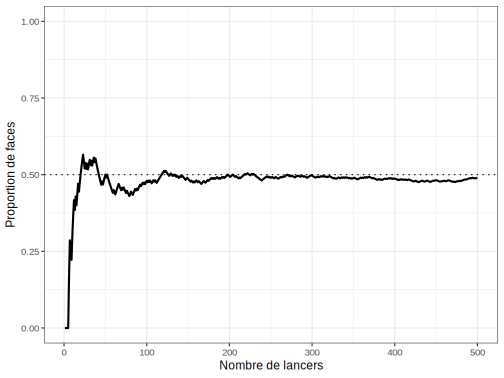
\includegraphics[width=0.75\linewidth]{IMSB_files/figure-latex/frequency-1} 

}

\caption{Illustration de l'interprétation fréquentiste du concept de probabilité. Lorsque le nombre d'essais augmente (en abscisse), la fréquence relative (en ordonnée) converge vers la probabilité d'obtenir Face.}\label{fig:frequency}
\end{figure}

La Figure \ref{fig:frequency} illustre l'\textbf{interprétation fréquentiste} du concept de probabilité en montrant que la fréquence relative converge vers une fréquence donnée (la ``probabilité'') quand le nombre d'essais augmente. Une conséquence importante de cette définition est que le concept de probabilité s'applique uniquement aux \textbf{collectifs} (i.e., aux séquences), et non aux événements singuliers. La probabilité est définie comme la limite d'une fréquence relative, et ne permet pas de parler de la probabilité d'un événement unique.

L'interprétation fréquentiste rencontre d'autres problèmes, comme celui de la classe de référence. Considérons par exemple la question suivante : ``Quelle est la probabilité que je vive jusqu'à 80 ans ?'' Pour répondre à cette question, nous avons besoin de définir la classe de référence à partir de laquelle l'individu examiné (``je'') provient. Autrement dit, je peux estimer la probabilité qu'un individu ayant mes caractéristiques vive jusqu'à 80 ans, mais il faut d'abord déterminer quelles sont les caractéristiques importantes au regard de la question posée. Selon mon sexe biologique, ma nationalité, ou mon statut socio-économique, la réponse à cette question peut varier drastiquement. L'interprétation fréquentiste ne propose pas de procédure stricte permettant de définir la classe de référence pertinente.

Par ailleurs, cette définition ne s'applique pas directement aux évènements qui ne peuvent pas se répéter. Par exemple, quelle est la probabilité que j'apprenne quelque chose pendant cette formation ? La réponse à cette question ne peut s'établir qu'en considérant des facteurs extérieurs à la question (e.g., le niveau de connaissance a priori), et ne peut pas reposer sur une évaluation sur le long-terme de la fréquence d'occurrence de l'événement ``apprendre quelque chose'' (cela n'aurait pas de sens de refaire la formation 1000 fois pour calculer le nombre de fois où on aura appris quelque chose).

Une autre limite importante de l'interprétation fréquentiste est la question de la résolution (ou précision) du calcul de cette probabilité. À partir de combien de lancers (d'une pièce par exemple) a-t-on une bonne approximation de la probabilité ? On sait qu'une classe finie d'événements de taille \(n\) ne peut produire que des fréquences relatives de précision \(1/n\). Jusque quand devrions-nous donc continuer ``d'échantillonner le long-terme'' avant d'avoir une estimation précise de la probabilité ?

\hypertarget{interpruxe9tation-propensionniste}{%
\subsubsection{Interprétation propensionniste}\label{interpruxe9tation-propensionniste}}

Selon l'interprétation propensionniste du concept de probabilité, les propriétés fréquentistes (i.e., à long terme) des objets (e.g., une pièce) seraient provoquées par des \emph{propriétés physiques intrinsèques} aux objets. Par exemple, une pièce biaisée va engendrer une fréquence relative (et donc une probabilité, selon l'interprétation fréquentiste) biaisée en raison de ses propriétés physiques. Pour les propensionnistes, les probabilités représentent ces caractéristiques intrinsèques, ces \textbf{propensions} à générer certaines fréquences relatives, et non les fréquences relatives en elles-mêmes.

Une conséquence intéressante de cette définition (et un progrès par rapport à l'interprétation fréquentiste) est que ces propriétés sont les propriétés d'événements individuels\ldots{} et non de séquences ! L'interprétation propensionniste nous permet donc de parler de la probabilité d'événements uniques.

\hypertarget{interpruxe9tation-logique}{%
\subsubsection{Interprétation logique}\label{interpruxe9tation-logique}}

L'interprétation logique du concept de probabilité, comme l'interprétation classique, postule que les probabilités peuvent être déterminées a priori en examinant les caractéristiques du système étudié (e.g., les caractéristiques de l'objet, l'ensemble des événements possibles, etc). Cependant, contrairement à l'interprétation classique, l'interprétation logique permet de rendre compte des événements non équiprobables. Cette interprétation se propose de réaliser cet objectif en généralisant la logique binaire (vrai / faux) au monde probabiliste, en étudiant le degré de support logique fourni par un ensemble de preuves pour une hypothèse donnée. Considérons par exemple l'argument logique ci-dessous.

\textbf{Prémisse n°1} : Considérons une salle dans laquelle sont présents 10 étudiants

\textbf{Prémisse n°2} : Neuf étudiants portent un t-shirt vert

\textbf{Prémisse n°3} : Un étudiant porte un t-shirt rouge

\textbf{Prémisse n°4} : Une personne est tirée au sort\ldots{}

\par

\noindent

\rule{\textwidth}{1pt}

\textbf{Conclusion n°1} : L'étudiant tiré au sort porte un t-shirt

Cette conclusion est \emph{vraie} et l'argument qui y est attachée est \emph{valide}. Pour rappel, on dit qu'un argument est \emph{valide} lorsqu'il n'existe aucune situation logiquement possible dans laquelle tous les prémisses de l'argument soient vrais et sa conclusion fausse (\protect\hyperlink{ref-talbot_critical_2015}{Talbot, 2015}). Autrement dit, si on considère les prémisses 1 à 4 comme vrais, alors il est (logiquement) impossible pour cette conclusion d'être fausse.

\par

\noindent

\rule{\textwidth}{1pt}

\textbf{Conclusion n°2} : L'étudiant tiré au sort porte un t-shirt rouge

Cette conclusion est \emph{fausse} et l'argument qui y est attachée est \emph{invalide.}

\par

\noindent

\rule{\textwidth}{1pt}

\textbf{Conclusion n°3} : L'étudiant tiré au sort porte un t-shirt vert

Cette conclusion est également \emph{fausse} et l'argument qui y est attaché est \emph{invalide}. Cependant, on pourrait dire intuitivement que cette conclusion est ``un peu moins fausse'' que la conclusion précédente (je m'excuse en avance pour les logiciens qui me lisent), dans le sens où elle est ``plus fortement'' impliquée par les prémisses 1 à 4 que la conclusion n°2.

Bien que les règles de la logique formelle n'autorisent pas des conclusions à être ``plus ou moins vraies'', l'interprétation logique du concept de probabilité cherche justement à étendre les règles de la logique aux événements continus, et se propose d'utiliser le langage des probabilités dans ce but. Autrement dit, la probabilité représente donc le \emph{degré de support logique} qu'une conclusion peut avoir, relativement à un ensemble de prémices (\protect\hyperlink{ref-carnap_logical_1950}{Carnap, 1950}; \protect\hyperlink{ref-keynes_treatise_1921}{Keynes, 1921}).

Une conséquence intéressante de cette interprétation est que toute probabilité est \textbf{conditionnelle}, que ce soit à de l'information a priori ou, par exemple, à un ensemble de prémisses.

\hypertarget{interpruxe9tation-bayuxe9sienne}{%
\subsubsection{Interprétation bayésienne}\label{interpruxe9tation-bayuxe9sienne}}

Selon l'interprétation bayésienne (subjective), la probabilité est \textbf{une mesure du degré de croyance} (ou \emph{crédence}) ou d'\emph{incertitude}. Un événement \emph{certain} aura donc une probabilité de 1 et un événement \emph{impossible} aura une probabilité de 0.

\begin{quote}
So to assign equal probabilities to two events is not in any way an assertion that they must occur equally often in any ``random experiment''; as Jeffrey emphasized, it is only a formal way of saying ``I don't know'' (\protect\hyperlink{ref-jaynes_bayesian_1986}{Jaynes, 1986}).
\end{quote}

Pour parler de probabilités, dans ce cadre, nous n'avons donc plus besoin de nous référer à la limite d'occurrence d'un événement (à sa fréquence). La probabilité est un concept abstrait faisant référence à un état de connaissance et / ou permettant de quantifier l'incertitude liée à cet état de connaissance.

\hypertarget{interpruxe9tations-probabilistes---ruxe9sumuxe9}{%
\subsubsection{Interprétations probabilistes - résumé}\label{interpruxe9tations-probabilistes---ruxe9sumuxe9}}

Pour résumer, les différentes interprétations discutées ci-dessus peuvent être classées dans deux grandes catégories :

\begin{quote}
\textbf{Interprétation épistémique} : toute probabilité est conditionnelle à de l'information disponible (e.g., prémisses ou données). La probabilité est utilisée comme moyen de quantifier l'incertitude.

Interprétation logique (e.g., Keynes, Carnap), interprétation bayésienne (e.g., Jeffreys, de Finetti, Savage).
\end{quote}

\begin{quote}
\textbf{Interprétation physique} : les probabilités dépendent d'un état du monde, de caractéristiques physiques, elles sont indépendantes de l'information disponible (ou de l'incertitude).

Interprétation classique (e.g., Laplace, Bernouilli, Leibniz), interprétation fréquentiste (e.g., Venn, Reichenbach, von Mises).
\end{quote}

Les plus curieux d'entre vous seront ravis de trouver plus d'informations dans cet excellent article de la \emph{Stanford Encyclopedia of Philosophy} (\protect\hyperlink{ref-sep-probability-interpret}{Hájek, 2019}) sur les différentes interprétations du concept de probabilité.

\hypertarget{logique-et-raisonnement-scientifique}{%
\section{Logique et raisonnement scientifique}\label{logique-et-raisonnement-scientifique}}

\hypertarget{introduction-uxe0-la-logique}{%
\subsection{Introduction à la logique}\label{introduction-uxe0-la-logique}}

Le but de cette section est de proposer une courte (et très incomplète) introduction à la logique, afin de pouvoir analyser dans une section ultérieure l'argument central de l'inférence fréquentiste et d'illustrer les similarités entre la logique et le fonctionnement de l'inférence bayésienne. Commençons tout d'abord commencer par définir les termes utilisés (cf. \protect\hyperlink{ref-talbot_critical_2015}{Talbot, 2015}).

\begin{definition}
\protect\hypertarget{def:argument}{}\label{def:argument}Un \emph{argument} est un ensemble de propositions dans lequel une proposition est affirmée sur la base d'autres propositions.
\end{definition}

Un argument (du moins tel que défini ici) est donc composé de différentes propositions. Parmi ces propositions, certaines vont être utilisées pour \emph{affirmer} une autre proposition.

\begin{definition}
\protect\hypertarget{def:concusion}{}\label{def:concusion}La \emph{conclusion} est l'affirmation faite sur la base d'autres propositions.
\end{definition}

\begin{definition}
\protect\hypertarget{def:prémisse}{}\label{def:prémisse}Les \emph{prémisses} d'un argument sont les raisons offertes qui permettent d'affirmer la conclusion.
\end{definition}

Pour résumer, un \emph{argument} est un ensemble de propositions, parmi lesquelles des \emph{prémisses} sont utilisées pour affirmer une \emph{conclusion}. Les propositions qui composent un \emph{argument} (i.e., les prémisses et la conclusion) peuvent être \emph{vraies} ou \emph{fausses} mais l'argument ne peut pas être \emph{vrai} ou \emph{faux}. Un argument est seulement \emph{valide} ou \emph{invalide}.

\begin{definition}
\protect\hypertarget{def:valide}{}\label{def:valide}Un argument est dit \emph{valide} si et seulement si il n'existe aucune situation logiquement possible dans laquelle tous les prémisses de l'argument soient vrais et sa conclusion fausse.
\end{definition}

\begin{definition}
\protect\hypertarget{def:invalide}{}\label{def:invalide}Un argument est dit \emph{invalide} si et seulement si il existe aucune situation logiquement possible dans laquelle tous les prémisses de l'argument soient vrais et sa conclusion fausse.
\end{definition}

Pour résumer, un argument est un ensemble de \emph{propositions}, dont certaines d'entre elles (les prémisses) sont utilisées pour affirmer (ou justifier) une autre (la conclusion). Ces propositions peuvent être vraies ou fausses mais un argument peut seulement être \emph{valide} ou \emph{invalide}. Un argument est dit \emph{valide} lorsqu'il est logiquement \emph{impossible} pour la conclusion d'être fausse (sachant que les prémisses sont \emph{vraies}).

\hypertarget{quelques-syllogismes-connus}{%
\subsection{Quelques syllogismes connus}\label{quelques-syllogismes-connus}}

\begin{figure}[!htb]

{\centering \includegraphics[width=0.5\linewidth]{figures/penguin} 

}

\caption{Un pingouin s'essayant à la logique. Source : https://www.pinterest.com/pin/465418942711158498/.}\label{fig:penguin}
\end{figure}

Un syllogisme est un raisonnement logique qui met en relation \emph{au moins} trois propositions : au moins deux prémisses et une conclusion. Afin d'illustrer les définitions proposées ci-dessus, nous allons maintenant examiner quelques exemples. Savez-vous reconnaître les arguments valides et invalides ?

\textbf{Argument n°1}

\begin{itemize}
\tightlist
\item
  Prémisse n°1 : Si un suspect ment, il transpire.
\item
  Prémisse n°2 : (On observe que) Ce suspect transpire.
\item
  Conclusion : Par conséquent, ce suspect ment.
\end{itemize}

Cet argument est \emph{invalide} car (on applique la définition \ref{def:valide}) il existe des situations dans lesquelles à la fois les prémisses 1 et 2 sont vraies, et pourtant la conclusion est fausse. Par exemple, il se peut que le suspect transpire pour d'autres raisons que le mensonge (e.g., la température de la salle d'interrogatoire).

\textbf{Argument n°2}

\begin{itemize}
\tightlist
\item
  Prémisse n°1 : Si un suspect transpire, il ment.
\item
  Prémisse n°2 : (On observe que) Ce suspect ne transpire pas.
\item
  Conclusion : Par conséquent, ce suspect ne ment pas.
\end{itemize}

Cet argument est également \emph{invalide} car il existe des situations dans lesquelles à la fois les prémisses 1 et 2 sont vraies, et pourtant la conclusion est fausse. Par exemple, il se peut que le suspect fasse partie des gens qui ne transpirent pas lorsqu'ils mentent.

\textbf{Argument n°3}

\begin{itemize}
\tightlist
\item
  Prémisse n°1 : Tous les menteurs transpirent.
\item
  Prémisse n°2 : (On observe que) Ce suspect ne transpire pas.
\item
  Conclusion : Par conséquent, ce suspect n'est pas un menteur.
\end{itemize}

Cet argument est \emph{valide} car il n'existe aucune situation dans laquelle à la fois les prémisses 1 et 2 sont vraies et la conclusion serait fausse. Autrement dit, si les prémisses 1 et 2 sont vraies, il est \emph{logiquement impossible} pour la conclusion d'être fausse. Nous allons maintenant examiner quelques raisonnements valides et invalides connus afin de nous aider à les repérer plus facilement.

\hypertarget{arguments-invalides}{%
\subsubsection{Arguments invalides}\label{arguments-invalides}}

Le premier raisonnement fallacieux que nous allons étudier est connu comme le sophisme de l'\textbf{affirmation du conséquent}. Ce raisonnement vise à inférer la réalisation d'un \emph{antécédent} sur la base de la réalisation du \emph{conséquent.} Considérons l'exemple suivant :

\begin{itemize}
\tightlist
\item
  Prémisse n°1 : S'il a plu, alors le sol est mouillé (A implique B).
\item
  Prémisse n°2 : Le sol est mouillé (B).
\item
  Conclusion : Donc il a plu (A).
\end{itemize}

Dans cet argument, le prémisse n°1 nous dit que l'antécédent (A) implique le conséquent (B). Le prémisse n°2 \emph{affirme} le conséquent B. La conclusion consiste à affirmer l'antécédent A sur la base de ces deux prémisse. Or cet argument est invalide, car (en l'occurrence) le sol pourrait être mouillé pour d'autres raisons que la pluie. Il s'agit du même genre de raisonnement que l'argument n°1 discuté dans la section précédente et il peut s'écrire dans une forme générale de la manière suivante :

\[\dfrac{A \Rightarrow B, \ B}{A}\]

où \(A \Rightarrow B\) se lit ``A implique B'' et se comprend comme dans la phrase ``Si A, alors B''.

Un deuxième argument fallacieux relativement répandu est connu comme le sophisme de la \textbf{négation de l'antécédent} et consiste à affirmer une négation du conséquent (i.e., non B) sur la base d'une négation de l'antécédent (i.e., non A). Considérons l'exemple suivant :

\begin{itemize}
\tightlist
\item
  Prémisse n°1 : S'il a plu, alors le sol est mouillé (A implique B).
\item
  Prémisse n°2 : Il n'a pas plu (non A).
\item
  Conclusion : Donc le sol n'est pas mouillé (non B).
\end{itemize}

Dans cet exemple comme dans le précédent, le prémisse n°1 nous dit que l'antécédent (A) implique le conséquent (B). Le prémisse n°2 affirme une négation de l'antécédent (i.e., non A ou \(\neg A\)). La conclusion consiste à affirmer une négation du conséquence (i.e., \(\neg B\)) sur la base de ces deux prémisses. Cet argument est également invalide car (en l'occurrence) le sol pourrait être mouillé pour d'autres raisons que le pluie. Autrement dit :

\[\dfrac{A \Rightarrow B, \ \neg A}{\neg B}\]

où \(\neg A\) représente la négation de A (i.e., non A).

\hypertarget{arguments-valides}{%
\subsubsection{Arguments valides}\label{arguments-valides}}

Attardons nous maintenons sur deux des raisonnements valides les plus connus. Le premier est connu comme le \textbf{modus ponens} et consiste à déduire un conséquent sur la base d'une implication (e.g., A implique B) et de l'affirmation d'un antécédent. Considérons l'exemple suivant :

\begin{itemize}
\tightlist
\item
  Prémisse n°1 : Si on est lundi, alors John ira au travail (A implique B).
\item
  Prémisse n°2 : On est lundi (A).
\item
  Conclusion : Donc John ira au travail (B).
\end{itemize}

Comme dans les deux exemples précédents, le prémisse n°1 nous dit que l'antécédent (A) implique le conséquent (B). Le prémisse n°2 \emph{affirme} l'antécédent A. La conclusion consiste à affirmer le conséquent B sur la base de ces deux prémisse. Cet argument est \emph{valide} (cf.~définition \ref{def:valide}) car il n'existe aucune situation \emph{logiquement possible} dans laquelle les deux prémisses serait vrais et la conclusion fausse. Autrement dit, cet argument est valide car il est \emph{impossible} pour la conclusion d'être fausse, sachant que les prémisses sont vrais. Le modus ponens peut s'écrire de la manière suivante :

\[\dfrac{A \Rightarrow B, \ A}{B} \cdot\]

Le deuxième argument valide que nous allons discuter est connu comme le \textbf{modus tollens}, dont l'importance s'avère capitale dans le raisonnement scientifique, ou du moins dans sa version idéalisée (cf.~section suivante). Cet argument consiste à déduire la négation de l'antécédent sur la base d'une implication et de la négation du conséquent. Considérons l'exemple suivant :

\begin{itemize}
\tightlist
\item
  Prémisse n°1 : Si mon chien détecte un intrus, alors il aboie (A implique B).
\item
  Prémisse n°2 : Mon chien n'a pas aboyé (non B).
\item
  Conclusion : Donc il n'a pas détecté d'intrus (non A).
\end{itemize}

Comme dans les exemples précédents, le prémisse n°1 nous dit que l'antécédent (A) implique le conséquent (B). Le prémisse n°2 affirme la ngation du conséquent (i.e., non B). La conclusion consiste à affirmer la négation de l'antécédent (i.e., non A) sur la base de ces deux prémisses. Cet argument est \emph{valide} (cf.~définition \ref{def:valide}) car il n'existe aucune situation \emph{logiquement possible} dans laquelle les deux prémisses serait vrais et la conclusion fausse. Autrement dit, cet argument est valide car il est \emph{impossible} pour la conclusion d'être fausse, sachant que les prémisses sont vrais. Dans notre exemple, si le chien n'a pas aboyé, c'est \emph{nécessairement} qu'il n'a pas détecté d'intrus. Cependant, cela ne veut pas dire qu'aucun intrus a visité notre maison, seulement que le chien n'a pas détecté d'intrus. Le modus tollens peut s'écrire de la manière suivante :

\[\dfrac{A \Rightarrow B, \ \neg B}{\neg A}\]

Ayant défini ce qu'est un argument, ce qui le compose et ce qui fait sa validité, nous disposons maintenant des outils nécessaires afin d'étudier la ``logique'' du raisonnement scientifique, et d'essayer de voir la place occupée par l'analyse de données dans ce raisonnement.

\hypertarget{quest-ce-quune-thuxe9orie-scientifique}{%
\subsection{Qu'est-ce qu'une théorie scientifique ?}\label{quest-ce-quune-thuxe9orie-scientifique}}

Qu'est-ce qu'une théorie scientifique ? D'un point de vue très général, une théorie scientifique peut être définie comme un ensemble de propositions logiques qui postulent des relations causales entre des phénomènes observables. Dans un premier temps, ces propositions sont formulées en termes abstraits et généraux (e.g., ``tout objet répond à la force de gravité de manière similaire''), mais mènent ensuite à des propositions concrètes et testable empiriquement (e.g., ``la vitesse de chute de deux objets devrait être la même, toute chose étant égale par ailleurs''). Il existe cependant de nombreux ``types'' de théories scientifiques. Par exemple, P. E. Meehl (\protect\hyperlink{ref-meehl_what_1986}{1986}) liste trois types de théories :

\begin{itemize}
\item
  \emph{Functional-dynamic theories} : les théories qui relient ``les états aux états'' ou ``les événements aux événements''. Par exemple, ce type de théorie décrit comment un changement sur une variable affecte une ou plusieurs autres variable(s).
\item
  \emph{Structural-compositional theories} : les théories qui expliquent ``de quoi est composé quelque chose'', de quels genres d'objets un plus gros objet est fait (i.e., sa structure), ou comment ces différentes parties sont assemblées.
\item
  \emph{Evolutionary theories} : les théories qui s'intéressent à l'histoire et au développement des choses (e.g., la théorie de l'évolution, la chute de Rome, etc).
\end{itemize}

Malgré cette diversité, et sans consensus clair sur ce qui fait une bonne ou une mauvaise théorie, la philosophie des sciences nous offre cependant des outils \emph{conceptuels} utiles pour \emph{évaluer} les théories, identifier ce qui les rend plus ou moins ``fortes'', et évaluer ce qui fait un \emph{test sévère} d'une théorie. Mais comment-on pouant nous évaluer les théories et comment créer des test sévères et pertinents ?

\hypertarget{on-ne-peut-pas-les-confirmer}{%
\subsubsection{On ne peut pas les confirmer}\label{on-ne-peut-pas-les-confirmer}}

Un premier ``problème'' avec les théories scientifiques est que nous ne pouvons pas les ``confirmer''. En effet, selon Campbell (\protect\hyperlink{ref-campbell_meehlian_1990}{1990}), le raisonnement scientifique (naif) aurait la forme logique suivante :

\begin{itemize}
\item
  Prémisse n°1 : Si la théorie de Newton (A) est ``vraie'', alors on devrait observer observer que les marées ont la période B, la trajectoire de Mars la forme C, la trajectoire d'une boule de canon la forme D, etc.
\item
  Prémisse n °2 : Nos observations confirment B, C, et D.
\item
  Conclusion : Donc la théorie de Newton est ``vraie''.
\end{itemize}

Or cet argument est invalide. Comme nous l'avons vu dans la section précédente, il s'agit du raisonnement fallacieux d'affirmation du conséquent. Une manière de s'en rendre compte est de réprésenter visuellement la forme de cet argument (cf.~Figure \ref{fig:campbell}).

\begin{figure}[!htb]

{\centering \includegraphics[width=0.5\linewidth]{figures/campbell} 

}

\caption{Relation entre observations et théorie de la gravitation de Newton, selon Campbell (1990).}\label{fig:campbell}
\end{figure}

L'invalidité de cet argument provient de l'existence de la zone hachurée de la Figure \ref{fig:campbell}, qui contient les autres explications possibles pour les observations que nous avons réalisées. En d'autres termes, observer B, C, et D ne nous permet pas de conclure que la théorie de Newton (A) est vraie, car ces observations pourraient avoir été générées par d'autres phénomènes que ceux postulés par la théorie de Newton. Cependant, observer B, C, D peut tout de même être informatif, selon certaines conditions, au regard de la théorie de Newton. Par exemple, si nous n'avions pas observé B, C, et D, alors nous aurions pu conclure que A était fausse. Donc observer B, C, et D fait que A reste ``plausiblement vraie''. Une autre manière de le dire est que A a ``survécu'' au test des observations B, C, et D. Nous verrons un peu plus loin comment la capacité des théories à survivre à un test empirique peut être utilisé comme métrique d'évaluation des théories.

\hypertarget{on-ne-peut-pas-les-ruxe9futer-au-sens-strict}{%
\subsubsection{On ne peut pas les réfuter (au sens strict)}\label{on-ne-peut-pas-les-ruxe9futer-au-sens-strict}}

Armés de nos connaissances en logique, nous avons donc établi qu'une théorie scientifique ne peut pas être \emph{confirmée}. Peut-être pourrions nous alors les \emph{réfuter} ? A-t-on des moyens de montrer qu'une théorie est fausse ? Qu'est-ce que cela veut dire pour une théorie d'être ``fausse'' ? Selon la pensée influente de Popper, une théorie est falsifiable (ou réfutable) si et seulement si il existe au moins un falsificateur potentiel (i.e., au moins une proposition possible qui soit en contradiction logique avec elle). En d'autres termes, une théorie peut être considérée comme réfutable s'il peut être démontré qu'elle est fausse.

Notons au passage que la falsifiabilité de Popper concerne le problème de la \emph{démarcation} (c'est-à-dire ce qu'est la science et ce qui est la pseudoscience) et définit les pseudosciences comme étant composées de théories non falsifiables (c'est-à-dire des théories qui ne permettent pas d'être réfutées). Mais lorsqu'il s'agit de décrire \emph{comment} la science fonctionne (visée descriptive) ou comment la science \emph{devrait} fonctionner (visée prescriptive), le standard falsificationniste ne fonctionne pas vraiment. En fait, il est quasiment unanimement impossible d'appliquer le falsificationnisme déductif dans des contextes scientifiques concrets (\protect\hyperlink{ref-mcelreath_statistical_2016}{McElreath, 2016b}). Dans les sections suivantes, nous discutons de quatre problèmes qui nous empêchent de réfuter des théories, à savoir : i) la distinction entre modèle théorique et modèle statistique, ii) le problème de la mesure, iii) la nature probabiliste des hypothèses scientifiques, et enfin iv) le problème de Duhem-Quine.

\hypertarget{moduxe8les-thuxe9oriques-et-moduxe8les-statistiques}{%
\subsubsection{Modèles théoriques et modèles statistiques}\label{moduxe8les-thuxe9oriques-et-moduxe8les-statistiques}}

Un modèle statistique est un appareil utilisé pour relier, pour faire le lien entre un modèle théorique et certaines données. Il peut être défini comme une instanciation d'une théorie en un ensemble d'énoncés ou de propositions probabilistes (\protect\hyperlink{ref-rouder_interplay_2016}{Rouder et al., 2016}). En général, il n'existe pas de relation univoque entre modèles théoriques et modèles statistiques. Autrement dit, un modèle théorique donné peut être représenté (i.e., implémenté) par différents modèles statistiques et réciproquement, différents modèles statistiques peuvent être construits à partir du même modèle théorique. Par conséquent, la confirmation ou réfutation d'un modèle statistique ne permet pas l'induction strict au modèle théorique.

Par exemple, une pratique statistique courante en sciences expérimentales est le test d'hypothèse nulle fréquentiste (\emph{Null Hypothesis Significance Testing} ou NHST), qui consiste à tester une hypothèse nulle (souvent l'hypothèse d'absence d'effet) afin de confirmer (ou plutôt, corroborer) une hypothèse théorique alternative d'intérêt. Or, le fait de rejeter l'hypothèse d'absence d'effet ne fournit qu'une très faible \emph{corroboration} de l'hypothèse d'intérêt, comme de nombreuses théories peuvent potentiellement prédire un effet est non-nul. L'hypothèse d'absence d'effet (i.e., l'hypothèse que l'effet est précisémment égal à \(0\)) est beaucoup plus contraignante (restrictive) que l'hypothèse alternative selon laquelle l'effet n'est pas \(0\).

\hypertarget{le-probluxe8me-de-la-mesure}{%
\subsubsection{Le problème de la mesure}\label{le-probluxe8me-de-la-mesure}}

La logique de la réfutation est assez simple et repose sur la puissance du \emph{modus tollens}. Appliqué au raisonnement scientifique, cet argument être présenté de la manière suivante :

\begin{itemize}
\item
  Prémisse n °1 : Si ma théorie \(T\) est correcte, alors je devrais observer certaines données \(D\).
\item
  Prémisse n°2 : J'observe d'autres données que celles prédites par ma théorie \(\lnot D\).
\item
  Conclusion : Donc, ma théorie est fausse \(\lnot T\).
\end{itemize}

Cet argument est parfaitement valide pour les propositions logiques, qui peuvent être soit vraies, soit fausses. Cependant, le premier problème qui apparait lorsqu'on on applique ce raisonnement à des cas concrets de raisonnement scientifique est le problème de l'erreur d'observation (ou erreur de mesure). Toute observation est sujette à de l'erreur, surtout lorsqu'on étudie des phénomènes nouveaux (\protect\hyperlink{ref-mcelreath_statistical_2016}{McElreath, 2016b}).

Considérons un instant un exemple qui nous vient de Physique, lorsqu'a été rapportée l'observation de \href{https://en.wikipedia.org/wiki/Neutrino}{neutrinos} plus rapides que la vitesse de la lumière (\protect\hyperlink{ref-mcelreath_statistical_2016}{McElreath, 2016b}, \protect\hyperlink{ref-mcelreath_statistical_2020}{2020}). Selon Einstein, aucun objet ne peut voyager plus vite que la lumière. Par conséquent, l'observation de certaines particules (en l'occurrence des neutrinos) qui voyageraient à une vitesse supérieure à celel de la lumière pourraient être considérée comme une réfutation flagrante de la théorie de la relativité restreinte.

En 2011, une large équipe de physiciens de renommée internationale ont pourtant annoncé la détection de neutrinos voyageant plus rapidement quela vitesse de la lumière. De manière intéressante, la première réaction de la communauté scientifique ne fut pas d'annoncer que la théorie d'Einstein était réfutée. Bien au contraire, la plus grande partie de la communauté s'est demandée ``D'où est-ce que vient l'erreur dans les mesures réalisées par cette équipe ?'' (\protect\hyperlink{ref-mcelreath_statistical_2016}{McElreath, 2016b}, \protect\hyperlink{ref-mcelreath_statistical_2020}{2020}). L'équipe ayant réalisée ces mesures a de ses voeux appelé à des réplications indépendantes de leurs résultats. Deux ans plus tard et après plusieurs ré-analyses et réplications contradictoires, la communauté était unanime que les résultats qui semblaient contredire la théorie d'Einstein étaient en fait dû à une erreur de mesure (l'équipe ayant réalisé les premières mesures a réalisé plus tard que l'erreur provenait \href{https://profmattstrassler.com/articles-and-posts/particle-physics-basics/neutrinos/neutrinos-faster-than-light/opera-what-went-wrong/}{d'un câble mal branché}).

Cette anecdote de l'histoire des sciences nous apprend au moins deux choses. Premièrement, il est intéressant d'analyser la réaction de la communauté de l'annonce de ces résultats. La théorie de la relativité restreinte ayant accumulé de nombreux succès prédictis au cours du dernier siècle, la survenue d'une observation si dramatiquement incompatible avec la théorie était perçue comme hautement improbable aux yeux des experts. Cela nous renseigne sur la manière dont les théories scientifiques gagnent en ``crédence'' aux yeux d'une communauté d'expert, et également comme cette crédence ou l'historique d'une théorie affecte ou influence la manière d'interpréter les observations empiriques. Deuxièmement, cela souligne le fait qu'une observation ou un ensemble d'observation peut difficilement compter comme une réfutation stricte d'une théorique, car il existe (presque) toujours une probabilité de se tromper ou une erreur irréductible dans la précision de la mesure. De manière générale, le problème avec l'erreur de mesure est de savoir si la réfutation d'une théorie \(T\) par un ensemble d'observations \(D\) est véritable ou simplement superficielle. Sachant que toute mesure est sujette à de l'erreur, toute conclusion scientifique qui repose sur une ou des mesure(s) ne peut qu'apporter une réfutation partielle (exprimée en termes probabilistes) d'une théorie, et non une réfutation stricte (comme en logique formelle).

\hypertarget{hypothuxe8ses-probabilistes}{%
\subsubsection{Hypothèses probabilistes}\label{hypothuxe8ses-probabilistes}}

Un autre problème émerge lorsqu'on essaye d'appliquer le modus tollens aux hypothèses scientifiques. Ce problème (désigné comme ``illusion permanente'' par \protect\hyperlink{ref-gigerenzer_superego_1993}{Gigerenzer, 1993}) est que la plupart des hypothèses scientifiques ne sont pas vraiment de la forme ``tous les cygnes sont blancs'' mais sont plutôt de la forme suivante :

\begin{itemize}
\item
  Mon hypothèse est que 90\% des cygnes sont blancs.
\item
  Si mon hypothèse est correcte, alors on ne devrait \emph{probablement pas} observer des cygnes noirs.
\end{itemize}

Sachant cette hypothèse, que peut-on conclure si on observe un cygne noir ? Et bien pas grand chose. Un autre exemple classique en sciences expérimentales est celui de la logique du test d'hypothèse nulle (\protect\hyperlink{ref-cohen_earth_1994}{Cohen, 1994}) :

\begin{itemize}
\item
  Prémisse n°1 : Si l'hypothèse nulle est vraie, alors ces données sont peu probables.
\item
  Prémisse n °2 : On observe ces données.
\item
  Conclusion : Donc l'hypothèse nulle est improbable.
\end{itemize}

Cependant, à cause du prémisse probabiliste (prémisse n°1), cet argument est invalide et sa conclusion est fausse. Pour s'en rendre compte, considérons un autre exemple (\protect\hyperlink{ref-cohen_earth_1994}{Cohen, 1994}; \protect\hyperlink{ref-pollard_probability_1987}{Pollard \& Richardson, 1987}) :

\begin{itemize}
\item
  Prémisse n°1 : Si un individu est Américain, il est peu probable qu'il soit membre du Congrès.
\item
  Prémisse n°2 : Cet individu n'est pas membre du Congrès.
\item
  Conclusion : Cet individu n'est probablement pas Américain.
\end{itemize}

Cette conclusion est saugrenue est l'argument est invalide, car il oublie de considérer l'alternative, qui est que si cet individu n'était pas Américain, la probabilité qu'il soit membre du Congrès serait de 0. Cet argument est identique au précédent :

\begin{itemize}
\item
  Prémisse n°1 : Si l'hypothèse nulle est vraie, alors ces données sont peu probables.
\item
  Prémisse n °2 : On observe ces données.
\item
  Conclusion : Donc l'hypothèse nulle est improbable.
\end{itemize}

Et cet argument est invalide pour les mêmes raisons que le précédent, à savoir i) que le prémisse n°1 est probabiliste (et non discret) et ii) qu'il ne considère pas l'hypothèse alternative. Ainsi, même sans erreur de mesure, on se rend compte que le problème d'hypothèse probabiliste nous empêche de réfuter ce genre d'hypothèse via le modus tollens.

\hypertarget{forme-logique-du-test-expuxe9rimental-dune-thuxe9orie}{%
\subsubsection{Forme logique du test expérimental d'une théorie}\label{forme-logique-du-test-expuxe9rimental-dune-thuxe9orie}}

Un dernier (mais non des moindres) problème est connu comme la ``thèse de Duhem-Quine'' ou le ``problème de l'indétermination''. En pratique, lorsqu'une théorie \(T\) est testée, il est nécessaire de faire appel à des hypothèses sous-jacentes (i.e., non explicites) ou à d'autres théories. Ces théories ``auxiliaires'' nous aident à ``connecter'' la théorie d'intérêt \(T\) avec le ``monde réel'', afin de faire des préditions concrètes (e.g., ``les cygnes blancs et noirs passent la même proportion de leur temps à se ballader, donc la probabilité de les observer dans la nature devrait être égale''). Ces théories auxiliaires sont souvent des théories à propos des outils que nous utilisons (e.g., ``le BDI est ou un outil valide pour mesurer le niveau de symptômes dépressifs chez des patients souffrant de dépression chronique'').

Lorsque nous testons une théorie qui prédit que ``Si \(O_{1}\)'' (une manipulation expérimentale), ``Alors \(O_{2}\)'' (une observation prédite), ce que nous voulons dire en fait est que l'on devrait observer cette relation \emph{si et seulement si} tous les éléments auxiliaires sont corrects. Ainsi, la structure logique du test empirique d'une théorie \(T\) peut être décrit de la manière suivante (\protect\hyperlink{ref-meehl_appraising_1990}{Paul E. Meehl, 1990a}, \protect\hyperlink{ref-meehl_theoretical_1978}{1978}, \protect\hyperlink{ref-harlow_problem_1997}{1997}) :

\[(T \land A_{t} \land C_{p} \land A_{i} \land C_{n}) \to (O_{1} \supset O_{2})\]

où ``\(\land\)'' représente une conjonction (``et''), ``\(\to\)'' représente une déduction logique, et ``\(\supset\)'' représente l'implication logique (e.g., ``Si \(O_{1}\), Alors \(O_{2}\)''). \(A_{t}\) est une conjonction de théories auxiliares, \(C_{p}\) est connu comme le \emph{ceteribus paribus} (i.e., on postule qu'il n'existe pas de factuers extérieurs non pris en compte et qui pourraient ``masquer'' l'effet d'intérêt) \(A_{i}\) est une théorie auxiliaire concernant les outils utilisés pour mesurer l'effet d'intérêt, et \(C_{n}\) est un énoncé à propos des conditions particulières de l'expérience réalisée (i.e., on postule qu'il n'existe pas de bruit ou erreur systémtique dans le protocole expérimental).

En d'autres termes, une \emph{conjonction} de tous les éléments du côté gauche de la formule ci-dessus (ce qui inclut notre théorie \(T\)) implique la partie droite de la formule, c'est à dire ``Si \(O_{1}\), Alors \(O_{2}\)''. Si l'expérience réalisée nous révèle que cette relation ne tient pas, alors on aimerait pouvoir conclure que notre hypothèse \(T\) est réfutée (en appliquant le modus tollens).

Or, une négation de la partie droite de cette formule nous permet seulement d'affirmer une négation de l'\textbf{intégralité} de la partie gauche. Autrement dit, ne pas observer une prédiction empirique d'une théorie nous permet de réfuter l'ensemble \(T \land A_{t} \land C_{p} \land A_{i} \land C_{n}\), ce qui est très différent d'une réfutation de \(T\) (\protect\hyperlink{ref-meehl_appraising_1990}{Paul E. Meehl, 1990a}). En termes plus formels, une négation de la conjonction (de gauche) est logiquement équivalent à déclarer une disjonction des conjoints (i.e., soit l'un ou l'autre des composants de la partie gauche est faux).

Pour résumer, ne pas observer quelque chose qui était prédit par une théorie ne permet pas de montrer que cette théorie est fausse, mais cela permet de montrer que la conjonctions de la théorie et des hypothèses auxiliaires est fausse. Une conséquence des quatre problèmes soulevés dans cette section et que la réfutation d'une théorie scientifique n'est jamais logique, mais elle est \textbf{consensuelle} (\protect\hyperlink{ref-mcelreath_statistical_2016}{McElreath, 2016b}, \protect\hyperlink{ref-mcelreath_statistical_2020}{2020}). Une proposition théorique est considérée comme réfutée lorsqu'une communauté d'experts a accumulé un grand nombre de preuves variées, issus de protocoles et de groupes de recherches variés, au fil des décennies. Ce travail d'accumulation des preuves s'accompagne de discussions critiques indissociables du travail de développement théorique. En somme, la réfutation d'une théorie est un résultat social, issue d'une communauté d'experts, et n'est (presque) jamais le résultat d'une déduction logique formelle.

\hypertarget{test-dhypothuxe8se-nulle-et-raisonnement-scientifique}{%
\subsection{Test d'hypothèse nulle et raisonnement scientifique}\label{test-dhypothuxe8se-nulle-et-raisonnement-scientifique}}

Une croyance répandue en sciences expérimentales est que l'utilisation de la procédure NHST est bien alignée avec la philosophie scientifique de Popper (et implicitement, qu'il s'agit là de quelque chose de souhaitable). Cependant, le parallèle entre la procédure NHST et la philosophie Poppérienne est très approximatif. La logique de la procédure NHST peut être résumée de la manière suivante :

\begin{enumerate}
\def\labelenumi{\arabic{enumi}.}
\tightlist
\item
  On suppose l'hypothèse d'absence d'effet \(\mathcal{H}_{0}\).
\item
  On génère un nombre infini d'échantillons sous cette hypothèse.
\item
  On compare les données que nous avons observées dans notre expérience à la distribution contrefactuelle des données sous l'hypothèse nulle \(\mathcal{H}_{0}\).
\end{enumerate}

Si les données observées semblent suffisamment invraisemblables conditionnellement à \(\mathcal{H}_{0}\) (où ``suffisamment'' correspond au niveau \(\alpha\) du test), nous pouvons rejeter l'hypothèse nulle en toute sécurité et considérer ce rejet comme une corroboration de l'hypothèse alternative \(\mathcal{H}_{1}\) (quelle que soit l'hypothèse alternative).

En d'autres termes, la seule hypothèse réellement testée (dans la procédure NHST classique) est l'hypothèse nulle, qui est rarement d'intérêt pour le chercheur en train de la tester. Ainsi, afin de réellement aligner cette procédure avec la méthode falsificationniste, il faudrait tester les prédictions de l'hypothése théorique \(\mathcal{T}\) réellement d'intérêt, et non les prédictions d'une hypothèse épouvantail \(\mathcal{H}_{0}\).\footnote{À ce propos, et comme nous le verrons un peu plus tard, il est possible et relativement facile de généraliser la procédure de calcul des p-valeurs à n'importe quel modèle statistique dans le cadre bayésien, voir par exemple cet article de blog : \url{http://www.barelysignificant.com/post/ppc/}.} Comme résumé par P. E. Meehl (\protect\hyperlink{ref-meehl_what_1986}{1986}) :

\begin{quote}
``{[}\ldots{]} we have been brainwashed by Fisherian statistics into thinking that refutation of H0 is a powerful way of testing substantive theories''.
\end{quote}

Pour résumer, Fidler et al. (\protect\hyperlink{ref-fidler_epistemic_2018}{2018}) décrivent quatre raisons qui questionne le parallèle entre la procédure NHST et la méthode falficationniste.

\begin{enumerate}
\def\labelenumi{\arabic{enumi}.}
\item
  L'hypothèse nulle \(\mathcal{H}_{0}\) (ou plutôt la \emph{nil hypothesis}, c'est à dire l'hypothèse que la valeur du paramètre testé est précisément \(0\)) est très probablement fausse car en sciences sociales en particulier ``tout tend à êtr associé avec tout'', un phénomène également connu comme le \emph{crud factor} (\protect\hyperlink{ref-meehl_why_1990}{Paul E. Meehl, 1990b}).
\item
  La procédure NHST ne teste pas réellement l'hypothèse d'intérêt \(\mathcal{T}\), mais seulement l'hypothèse épouvantail \(\mathcal{H}_{0}\).
\item
  De nombreuses hypothèses théories sous-jacentes ne sont pas assez bien développées ou formalisées et ne permettent pas de formuler des hypothèses statistiques.
\item
  Même si tous les points précédents ont été résolus, nous aurions encore besoin de soumettre ces hypothèses à des tests sévères, ce qui nécessiterait des études bien alimentées et bien conçues, ce qui n'est pas la norme actuelle \footnote{La puissance statistique moyenne des tests d'hypothèse réalisés en Psychologie est estimée à moins de 50\% (e.g., \protect\hyperlink{ref-szucs_empirical_2017-1}{Szucs \& Ioannidis, 2017}).}.
\end{enumerate}

Le point n°2 soulevé ci-dessus nous dit que la procédure NHST ne suit pas le falsificationnisme Poppérien car il ne soumet pas la théorie testée à un risque de falification \emph{sévère}, mais seulement à un danger très faible. En d'autres termes, le test d'hypothèse nulle (tel que pratiqué dans la procédure NHST classique) ne soumet pas la théorie sous-jacente (i.e., celle qu'on vise à évaluer via le test de l'hypothèse statistique dérivée de cette première) à un test fort (\protect\hyperlink{ref-meehl_appraising_1990}{Paul E. Meehl, 1990a}, \protect\hyperlink{ref-meehl_theory-testing_1967}{1967}, \protect\hyperlink{ref-harlow_problem_1997}{1997}). Autrement dit, étant donné que l'hypothèse nulle est facilement réfutée, l'hypothèse alternative est facilement corroborée statistiquement, et donc peu corroborée au niveau théorique.

Ceci étant dit, cette critique porte sur une manière d'utiliser la procédure NHST (qui est aujourd'hui la plus répandue en Psychologie), mais ce n'est pas la seule manière d'utiliser cette procédure. On pourrait très bien utiliser cette procédure afin d'essayer de réfuter notre hypothèse d'intérêt \(\mathcal{T}\). Paul E. Meehl (\protect\hyperlink{ref-meehl_theory-testing_1967}{1967}) distingue entre l'usage \emph{fort} et \emph{faible} du test d'hypothèse nulle en comparant l'usage de la procédure NHST en physique et en psychologie. L'usage \emph{faible} du test d'hypothèse nulle, décrit ci-dessus, correspond à tenter de réfuter une hypothèse nulle qui ne nous intéresse pas afin de corroborer une hypothèse alternative d'intérêt.

L'usage fort du test d'hypothèse nulle nécessite cependant d'avoir une théorie suffisamment développée, à même de prédire une valeur numérique précise pour une observation, ou tout du moins un intervalle réduit de valeurs possibles, ou alors certaines formes de fonctions (e.g., quadratique ou cubique) entre les variables d'intérêt (\protect\hyperlink{ref-harlow_problem_1997}{Paul E. Meehl, 1997}). Dans ce genre de situation, le test d'hypothèse nulle pourrait agir comme un test Poppérien \emph{risqué}, au sens où l'hypothèse testée est soumises à un risque élevé de réfutation (\protect\hyperlink{ref-harlow_problem_1997}{Paul E. Meehl, 1997}). Notons également que la procédure NHST peut être adaptée afin de réfuter des intervalles de valeurs, via les tests d'équivalence (\protect\hyperlink{ref-lakens_equivalence_2018}{Lakens et al., 2018}; \protect\hyperlink{ref-rogers_using_1993}{Rogers et al., 1993}) ou la procédure HDI+ROPE (\protect\hyperlink{ref-kruschke_doing_2015}{Kruschke, 2015}).

Bien entendu, dans certaines (rares) situations, l'hypothèse d'absence d'effet est théoriquement d'intérêt, et donc viser à réfuter cette hypothèse via un test d'hypothèse nulle représenterait une tentative sérieuse de réfutation. Par exemple il existe certaines théories en Psychologie qui prédisent que certains comportement seraient invariants selon certaines situations (\protect\hyperlink{ref-morey_beyond_2018}{Morey et al., 2018}). Ces hypothèses peuvent être testées \emph{sévèrement} par un test d'hypothèse nul, car ce dernier les exposerait à un haut risque de réfutation.

Pour résumer, la vision naïve du falsificationnisme consiste à penser que la science progresse par falsification logique (et que donc la statistique devrait viser la falsification). Cependant, comme discuté dans cette section, cette perspective se retrouve face à plusieurs problèmes difficilement surmontables, que nous résumons ci-dessous/

\begin{itemize}
\item
  Premier problème : Les hypothèses théoriques ne sont pas les modèles (hypothèses statistiques). Un modèle statistique est un appareil utilisé pour relier, pour faire le lien entre un modèle théorique et certaines données. Il peut être défini comme une instanciation d'une théorie en un ensemble d'énoncés ou de propositions probabilistes (\protect\hyperlink{ref-rouder_interplay_2016}{Rouder et al., 2016}).
\item
  Deuxième problème : En général, il n'existe pas de relation univoque entre modèles théoriques et modèles statistiques. Autrement dit, un modèle théorique donné peut être représenté (i.e., implémenté) par différents modèles statistiques et réciproquement, différents modèles statistiques peuvent être construits à partir du même modèle théorique. Par conséquent, la confirmation ou réfutation d'un modèle statistique ne permet pas l'induction strict au modèle théorique.
\item
  Troisième problème : Les hypothèses scientifique sont souvent probabilistes, ce qui invalide l'emploi du modus tollens.
\item
  Quatrième problème : Les mesures permettant de tester une théories sont sujette à des erreurs, ce qui empêche également la réfutation strictes d'hypothèses (cf.~l'anecdote des neutrinos).
\end{itemize}

Enfin, la falsification concerne le problème de la démarcation, pas celui de la méthode. La science est une technologie sociale, la falsification est \textbf{consensuelle}, et non pas logique.

\hypertarget{lapproche-par-comparaison-de-moduxe8les}{%
\subsection{L'approche par comparaison de modèles}\label{lapproche-par-comparaison-de-moduxe8les}}

En connaissance des limitations de l'approche par test d'hypothèse nulle telle que présentée dans la section précédente, nous adoptons dans ce livre une approche dite par \emph{comparaison de modèle}.

En bref, en place d'une approche mécanique du test d'hypothèse nulle, nous proposons une méthode qui met l'accent sur l'estimation de paramètres, la comparaison de modèles statistiques et théoriques (sensés et d'intérêt), et l'extension (amélioration) continuelle du modèle (\protect\hyperlink{ref-burnham_multimodel_2004}{Burnham \& Anderson, 2004}; e.g., \protect\hyperlink{ref-burnham_model_2002}{Burnham \& Anderson, 2002}; \protect\hyperlink{ref-cumming_new_2014}{Cumming, 2014}, \protect\hyperlink{ref-Cumming2012}{2012}; \protect\hyperlink{ref-gelman_bayesian_2013}{Gelman et al., 2013}; \protect\hyperlink{ref-gelman_data_2006}{Gelman \& Hill, 2006}; \protect\hyperlink{ref-judd_data_2009}{Judd et al., 2009}; \protect\hyperlink{ref-kruschke_doing_2015}{Kruschke, 2015}; \protect\hyperlink{ref-kruschke_bayesian_2018}{Kruschke \& Liddell, 2018a}, \protect\hyperlink{ref-kruschke_bayesian_2018-1}{2018b}; \protect\hyperlink{ref-R-rethinking}{McElreath, 2016a}). En d'autres notre approche est une approche de \textbf{modélisation statistique} plutôt qu'une approche de \textbf{test statistique} (e.g., \protect\hyperlink{ref-noel_psychologie_2015}{Noël, 2015}). Cette approche vise à modéliser le processus sous-jacent ayant généré les données observées (i.e., le \emph{processus de génération des données} ou PGD) plutôt qu'à tester si la valeur de certains paramètres d'un modèle inapproprié est égal à une valeur arbitraire (e.g., \(\theta = 0\)). Cette approche n'est cependant pas incompatible avec l'approche falsificationniste tel que décrite en philosophie des sciences. En effet, certains statisticiens bayésiens comme Gelman \& Shalizi (\protect\hyperlink{ref-gelman_philosophy_2013}{2013}) suggèrent que la réfutation des modèles statistiques joue un rôle important dans le processus de modélisation et d'amélioration des modèles (nous y reviendrons à plusieurs reprises, en particulier lorsque nous discuterons l'utilisation des \emph{prior} et \emph{posterior predictive checks}).

Afin d'illustrer l'approche par comparaison de modèles, considérons l'exemple suivant. On s'intéresse au lien entre deux variables aléatoires continues \(x\) et \(y\). On réalise une expérience et on collecte 10 observations nous permettant d'étudier cette relation. L'hypothèse de modélisation la plus classique est de postuler une relation linéaire entre \(x\) et \(y\). La droite minimisant la somme des erreurs au carré est représentée par la Figure \ref{fig:modelcomp2}.

\begin{figure}[!htb]

{\centering \includegraphics[width=0.75\linewidth]{IMSB_files/figure-latex/modelcomp2-1} 

}

\caption{Scatterplot des 10 observations obtenues dans notre expérience et droite des moindres carrés décrivant la relation entre x et y estimée sur la base de ces 10 observations.}\label{fig:modelcomp2}
\end{figure}

Cette description peut-être \emph{améliorée} (où ``améliorer'' consiste à réduire l'erreur) pour mieux prendre en compte les données qui s'écartent de la prédiction linéaire. La figure \ref{fig:modelcomp3} représente la prédiction d'un modèle polynomial (quadratique).

\begin{figure}[!htb]

{\centering \includegraphics[width=0.75\linewidth]{IMSB_files/figure-latex/modelcomp3-1} 

}

\caption{Prédiction quadratique décrivant la relation entre x et y estimée sur la base des 10 observations collectées pour notre expérience.}\label{fig:modelcomp3}
\end{figure}

Cette ``amélioration'' du modèle statistique via une augmentation de la complexité de ce dernier peut être poursuivi. On sait qu'un ensemble de \(N\) points peut être \emph{exhaustivement} (i.e., sans erreur) décrit par une fonction polynomiale d'ordre \(N - 1\) (cf.~Figure \ref{fig:modelcomp4}). Augmenter la complexité du modèle améliore donc la précision de notre description des données mais réduit également la généralisabilité de ses prédictions (il s'agit du dilemme classique entre biais et variance).

\begin{figure}[!htb]

{\centering \includegraphics[width=0.75\linewidth]{IMSB_files/figure-latex/modelcomp4-1} 

}

\caption{Différentes prédictions de complexité croissante estimées sur la base des 10 observations collectées pour notre expérience.}\label{fig:modelcomp4}
\end{figure}

Nous avons donc besoin d'outils qui prennent en compte le rapport entre la qualité de la description des données et la complexité du modèle, c'est à dire qui évaluent la parcimonie du modèle. Dans cette perspective, nous ferons au Chapitre 6 un détour par la théorie de l'information, qui nous permettra introduire des outils comme l'AIC (et ses différentes extensions).

Pour résumer, notre approche consistera donc à construire des modèles statistiques comme des implémentations mathématiques (probabilistes) de modèles théoriques que nous souhaitons comparer. L'inférence statistique bayésienne consistera à mettre à jour notre état de connaissance concernant les valeur des paramètres de ces modèles (mais également notre état de connaissance vis à vis de la validité relative de ces modèles) en fonction des données observées. Ces modèles seront comparés en fonction de i) leur puissance prédictive et ii) leur complexité. Au lieu d'essayer de réfuter un modèle épouvantail (i.e., l'hypothèse nulle), on comparera des modèles intrinsèquement intéressants, qu'on essayera de réfuter afin de les améliorer. La section suivante présente un premier exemple permettant de saisir l'idée centrale de l'inférence bayésienne.

\hypertarget{probluxe8me-du-sac-de-billes-mcelreath_statistical_2016}{%
\section{\texorpdfstring{Problème du sac de billes (\protect\hyperlink{ref-mcelreath_statistical_2016}{McElreath, 2016b})}{Problème du sac de billes (McElreath, 2016b)}}\label{probluxe8me-du-sac-de-billes-mcelreath_statistical_2016}}

Imaginons que nous disposions d'un sac contenant 4 billes. Ces billes peuvent être soit blanches, soit bleues. Nous savons qu'il y a précisément 4 billes, mais nous ne connaissons pas le nombre de billes de chaque couleur. Nous savons cependant qu'il existe cinq possibilités (que nous considérons comme nos \emph{hypothèses}) :

\[
\begin{aligned}
&\text{Hypothèse n°1 : } \LARGE \circ \circ \circ \circ \\
&\text{Hypothèse n°2 : } \LARGE \color{steelblue}{\bullet} \color{black}{\circ} \circ \circ \\
&\text{Hypothèse n°3 : } \LARGE \color{steelblue}{\bullet} \color{steelblue}{\bullet} \color{black}{\circ} \circ \\
&\text{Hypothèse n°4 : } \LARGE \color{steelblue}{\bullet} \color{steelblue}{\bullet} \color{steelblue}{\bullet} \color{black}{\circ} \\
&\text{Hypothèse n°5 : } \LARGE \color{steelblue}{\bullet} \color{steelblue}{\bullet} \color{steelblue}{\bullet} \color{steelblue}{\bullet} \\
\end{aligned}
\]

Le but est de déterminer quelle combinaison est la plus probable, \textbf{sachant certaines observations}. Imaginons que l'on tire trois billes à la suite, avec remise, et que l'on obtienne la séquence suivante : \(\LARGE \color{steelblue}{\bullet} \color{black}{\circ} \color{steelblue}{\bullet}\).

Cette séquence représente nos données. À partir de ces données, quelle \textbf{inférence} peut-on faire sur le contenu du sac ? En d'autres termes, que peut-on dire de la probabilité de chaque hypothèse ?

\hypertarget{uxe9numuxe9rer-les-possibilituxe9s}{%
\subsection{Énumérer les possibilités}\label{uxe9numuxe9rer-les-possibilituxe9s}}

Une stratégie consiste à compter le nombre de possibilités menant aux données obtenues à chaque tirage. Par exemple, si nous considérons l'hypothèse n°2 (i.e., on se place dans un cadre dans lequel cette hypothèse est ``vraie''), on peut représenter l'arbre des issues possibles. La Figure \ref{fig:garden1} représente ces différentes possibilités. Au premier tirage, selon l'hypothèse n°2, nous avions une chance sur 4 d'obtenir une bille bleue.

\begin{figure}[!htb]

{\centering \includegraphics[width=0.75\linewidth]{IMSB_files/figure-latex/garden1-1} 

}

\caption{Représentation de l'ensemble des issues possibles au premier tirage selon l'hypothèse n°2.}\label{fig:garden1}
\end{figure}

La Figure \ref{fig:garden2} représente l'ensemble des résultats possibles aux tirages 1 et 2 selon l'hypothèse n°2. On réalise qu'au deuxième comme au premier tirage, on avait une chance sur quatre d'obtenir une bille bleue. Par conséquent on avait \(1 \times (4 \times 1) = 4\) chances sur \(4^2 = 16\) d'obtenir deux billes bleues. De la même manière, on peut calculer qu'on avait \(1 \times 3\) chances sur \(4^2 = 16\) d'obtenir une bille bleue et une bille blanche. Autrement dit, 3 chemins mènent à la suite ``bille bleue puis bille blanche''.

\begin{figure}[!htb]

{\centering \includegraphics[width=0.75\linewidth]{IMSB_files/figure-latex/garden2-1} 

}

\caption{Représentation de l'ensemble des issues possibles aux premier et deuxième tirages selon l'hypothèse n°2.}\label{fig:garden2}
\end{figure}

La Figure \ref{fig:garden3} représente l'ensemble des résultats possibles aux tirages 1, 2, et 3 selon l'hypothèse n°2. On réalise qu'à chaque tirage on avait une chance sur quatre d'obtenir une bille bleue. Par conséquent on avait \(1 \times (4 \times 1) \times (4 \times 1) = 16\) chances sur \(4^3 = 64\) d'obtenir trois billes bleues. De la même manière, on peut calculer qu'on avait \(1 \times 3 \times 1\) chances sur \(4^3 = 64\) d'obtenir une bille bleue et une bille blanche. Autrement dit, 3 chemins mènent à la suite ``bille bleue puis bille blanche puis bille bleue''.

\begin{figure}[!htb]

{\centering \includegraphics[width=0.75\linewidth]{IMSB_files/figure-latex/garden3-1} 

}

\caption{Représentation de l'ensemble des issues possibles selon l'hypothèse n°2 sur l'ensemble des tirages.}\label{fig:garden3}
\end{figure}

La Figure \ref{fig:garden4} représente le nombre de ``chemins'' qui mènent au résultat obtenu et confirme que sous l'hypothèse n°2, \(3\) chemins sur \(4^{3} = 64\) conduisent au résultat obtenu. Qu'en est-il des autres hypothèses?

\begin{figure}[!htb]

{\centering \includegraphics[width=0.75\linewidth]{IMSB_files/figure-latex/garden4-1} 

}

\caption{Représentation de l'ensemble des issues possibles selon l'hypothèse n°2 sur l'ensemble des tirages. Les chemins menant aux données observées sont mis en avant.}\label{fig:garden4}
\end{figure}

La Figure \ref{fig:garden5} représente le nombre de chemins menant aux données observées pour les hypothèse n°2, n°3, et n°4.

\begin{figure}[!htb]

{\centering \includegraphics[width=0.75\linewidth]{IMSB_files/figure-latex/garden5-1} 

}

\caption{Représentation de l'ensemble des issues possibles selon les hypothèses n°2, n°3, et n°4 sur l'ensemble des tirages. Les chemins menant aux données observées sont mis en avant.}\label{fig:garden5}
\end{figure}

On peut ensuite comparer les hypothèses par leur \emph{propension} à mener aux données observées. Plus précisément, on peut comparer les hypothèses entre elles en comparant le nombre de chemins menant aux données pour chaque hypothèse (cf.~Tableau \ref{tab:hypothesis-comparison}).

\begin{table}[!htb]

\begin{center}
\begin{threeparttable}

\caption{\label{tab:hypothesis-comparison}Comparer des hypothèses en comparant le nombre de manières qu'elles ont de produire les données observées.}

\begin{tabular}{cc}
\toprule
Hypothèse & Façons d'obtenir les données\\
\midrule
$\LARGE \circ \circ \circ \circ$ & $0 \times 4 \times 0 = 0$\\
$\LARGE \color{steelblue}{\bullet} \circ \circ \circ$ & $1 \times 3 \times 1 = 3$\\
$\LARGE \color{steelblue}{\bullet} \color{steelblue}{\bullet} \circ \circ$ & $2 \times 2 \times 2 = 8$\\
$\LARGE \color{steelblue}{\bullet} \color{steelblue}{\bullet} \color{steelblue}{\bullet} \circ$ & $3 \times 1 \times 3 = 9$\\
$\LARGE \color{steelblue}{\bullet} \color{steelblue}{\bullet} \color{steelblue}{\bullet} \color{steelblue}{\bullet}$ & $4 \times 0 \times 4 = 0$\\
\bottomrule
\end{tabular}

\end{threeparttable}
\end{center}

\end{table}

On pourra conclure, au vu des données, que l'hypothèse n°4 est la plus \emph{plausible} car c'est l'hypothèse qui \textbf{maximise le nombre de manières possibles d'obtenir les données obtenues}.

\hypertarget{accumulation-duxe9vidence}{%
\subsection{Accumulation d'évidence}\label{accumulation-duxe9vidence}}

Jusque là, nous avons considéré que toutes les hypothèses étaient équiprobables a priori (suivant le \href{https://en.wikipedia.org/wiki/Principle_of_indifference}{principe d'indifférence}). Cependant, on pourrait avoir de l'information a priori, provenant de nos connaissances (e.g., concernant les particularités des sacs de billes) ou de données antérieures. Imaginons que nous tirions une nouvelle bille du sac. Comment pouvons-nous incorporer cette nouvelle donnée ?

Il suffit d'appliquer la même stratégie que précédemment, et de mettre à jour le dernier compte en le multipliant par ces nouvelles données (cf.~Tableau \ref{tab:accumulation}). Cette procédure illustre un mécanisme central de l'inférence bayésienne qui concerne l'accumulation d'information. Dans le cadre bayésien, cette accumulation se déroule naturellement, où le résultat de nouvelles analyses peut être naturellement incorporé au résultat d'analyses précédentes, pour mener à un état de connaissance mis à jour.

\begin{table}[!htb]

\begin{center}
\begin{threeparttable}

\caption{\label{tab:accumulation}Illustration de l'accumulation d'information dans le cadre bayésien.}

\begin{tabular}{cccc}
\toprule
Hypothèse & Façons de produire $\color{steelblue}{\bullet}$ & Compte précédent & Nouveau compte\\
\midrule
$\LARGE \circ \circ \circ \circ$ & $0$ & $0$ & $0 \times 0 = 0$\\
$\LARGE \color{steelblue}{\bullet} \circ \circ \circ$ & $1$ & $3$ & $3 \times 1 = 3$\\
$\LARGE \color{steelblue}{\bullet} \color{steelblue}{\bullet} \circ \circ$ & $2$ & $8$ & $8 \times 2 = 16$\\
$\LARGE \color{steelblue}{\bullet} \color{steelblue}{\bullet} \color{steelblue}{\bullet} \circ$ & $3$ & $9$ & $9 \times 3 = 27$\\
$\LARGE \color{steelblue}{\bullet} \color{steelblue}{\bullet} \color{steelblue}{\bullet} \color{steelblue}{\bullet}$ & $4$ & $0$ & $0 \times 4 = 0$\\
\bottomrule
\end{tabular}

\end{threeparttable}
\end{center}

\end{table}

\hypertarget{incorporer-un-prior}{%
\subsection{Incorporer un prior}\label{incorporer-un-prior}}

Supposons maintenant qu'un employé de l'usine de fabrication des billes nous dise que les billes bleues sont rares. Plus précisément, cet employé nous dit que pour chaque sac contenant 3 billes bleues, ils fabriquent deux sacs en contenant seulement deux, et trois sacs en contenant seulement une. Il nous apprend également que tous les sacs contiennent au moins une bille bleue et une bille blanche. On peut traduire ces informations en langage mathématique, en attribuant un poids de \(0\) pour les hypothèses n°1 et n°5, et en rendant l'hypothèse n°2 trois fois plus probable que l'hypothèses n°4, et l'hypothèse n°3 deux fois plus probable que l'hypothèse n°4 (cf.~Tableau \ref{tab:prior-table}).

\begin{table}[!htb]

\begin{center}
\begin{threeparttable}

\caption{\label{tab:prior-table}Illustration de l'intégration d'information a priori dans le cadre bayésien.}

\begin{tabular}{cccc}
\toprule
Hypothèse & Compte précédent & Prior usine & Nouveau compte\\
\midrule
$\LARGE \circ \circ \circ \circ$ & $0$ & $0$ & $0 \times 0 = 0$\\
$\LARGE \color{steelblue}{\bullet} \circ \circ \circ$ & $3$ & $3$ & $3 \times 3 = 9$\\
$\LARGE \color{steelblue}{\bullet} \color{steelblue}{\bullet} \circ \circ$ & $16$ & $2$ & $16 \times 2 = 32$\\
$\LARGE \color{steelblue}{\bullet} \color{steelblue}{\bullet} \color{steelblue}{\bullet} \circ$ & $27$ & $1$ & $27 \times 1 = 27$\\
$\LARGE \color{steelblue}{\bullet} \color{steelblue}{\bullet} \color{steelblue}{\bullet} \color{steelblue}{\bullet}$ & $0$ & $0$ & $0 \times 4 = 0$\\
\bottomrule
\end{tabular}

\end{threeparttable}
\end{center}

\end{table}

Cette procédure illustre encore une fois l'intégration d'information antérieure (on dira également \emph{a priori}), que ce soit empirique ou théorique, dans l'analyse de nouvelles données. Ce mécanisme est résumé par le célèbre dicton bayésien : \emph{Yesterday's posterior is today's prior} (\protect\hyperlink{ref-lindley_philosophy_2001}{Lindley, 2001}).

\hypertarget{des-uxe9numuxe9rations-aux-probabilituxe9s}{%
\subsection{Des énumérations aux probabilités}\label{des-uxe9numuxe9rations-aux-probabilituxe9s}}

Le théorème de Bayes (que nous présenterons formellement un peu plus tard) nous dit que la probabilité d'une hypothèse après avoir observé certaines données est proportionnelle au nombre de façons qu'a cette hypothèse de produire les données observées, multiplié par sa probabilité a priori.

\[
\Pr(\text{hypothèse} \ | \ \text{données}) \propto \Pr(\text{données} \ | \ \text{hypothèse}) \times \Pr(\text{hypothèse})
\]

Si l'on considère toutes les hypothèses comme étant équiprobables a priori (e.g., on leur accorde toutes une probabilité de 1), la \textbf{probabilité postérieure} de l'hypothèse \textbf{sachant les données observées et le prior} est obtenue en normalisant le produit \(\Pr(\text{données} \ | \ \text{hypothèse}) \times \Pr(\text{hypothèse})\) de la manière suivante :

\[
\Pr(\text{hypothèse} \ | \ \text{données}) = \frac{\Pr(\text{données} \ | \ \text{hypothèse}) \times \Pr(\text{hypothèse})}{\text{Somme des produits}}
\]

Où la somme des produits consiste à calculer le produit \(\Pr(\text{données} \ | \ \text{hypothèse}) \times \Pr(\text{hypothèse})\) pour toutes les hypothèses considérées et à calculer la somme de ces valeurs. Cette manipulation nous assure que la probabilité postérieure (i.e., \(\Pr(\text{hypothèse} \ | \ \text{données})\)) est bien une probabilité, c'est à dire une valeur numérique bornée entre \(0\) et \(1\).

Par exemple, si l'on définit \(p\) comme étant la proportion de billes bleues dans chaque hypothèse, alors on peut ré-exprimer chaque hypothèse en fonction de \(p\) (cf.~Tableau \ref{tab:enumeration-table}).

\begin{table}[!htb]

\begin{center}
\begin{threeparttable}

\caption{\label{tab:enumeration-table}Calcul de la probabilité postérieure d'une hypothèse.}

\begin{tabular}{cccc}
\toprule
Hypothèse & $p$ & Manières de produire les données & Probabilité postérieure\\
\midrule
$\LARGE \circ \circ \circ \circ$ & $0$ & $0$ & $0$\\
$\LARGE \color{steelblue}{\bullet} \circ \circ \circ$ & $0.25$ & $3$ & $0.15$\\
$\LARGE \color{steelblue}{\bullet} \color{steelblue}{\bullet} \circ \circ$ & $0.5$ & $8$ & $0.40$\\
$\LARGE \color{steelblue}{\bullet} \color{steelblue}{\bullet} \color{steelblue}{\bullet} \circ$ & $0.75$ & $9$ & $0.45$\\
$\LARGE \color{steelblue}{\bullet} \color{steelblue}{\bullet} \color{steelblue}{\bullet} \color{steelblue}{\bullet}$ & $1$ & $0$ & $0$\\
\bottomrule
\end{tabular}

\end{threeparttable}
\end{center}

\end{table}

Où la probabilité est calculée en divisant chaque valeur de la troisième colonne par la somme des valeurs de cette colonne. Autrement dit, en \texttt{R} :

\begin{Shaded}
\begin{Highlighting}[]
\NormalTok{ways }\OtherTok{\textless{}{-}} \FunctionTok{c}\NormalTok{(}\DecValTok{0}\NormalTok{, }\DecValTok{3}\NormalTok{, }\DecValTok{8}\NormalTok{, }\DecValTok{9}\NormalTok{, }\DecValTok{0}\NormalTok{)}
\NormalTok{ways }\SpecialCharTok{/} \FunctionTok{sum}\NormalTok{(ways)}
\end{Highlighting}
\end{Shaded}

\begin{verbatim}
## [1] 0.00 0.15 0.40 0.45 0.00
\end{verbatim}

Pour résumer, la probabilité postérieure représente la probabilité d'une hypothèse, \textbf{sachant} certaines données observées et certaines connaissances a priori. Cette probabilité postérieure est proportionnelle au produit de la probabilité des données sachant l'hypothèse (i.e., le nombre de manières qu'a l'hypothèse de produire les données) et de la probabilité a priori de l'hypothèse. Autrement dit et comme résumé par McElreath (\protect\hyperlink{ref-mcelreath_statistical_2016}{2016b}), ``\emph{Bayesian inference is really just counting and comparing of possibilities}''.

\hypertarget{rappels-de-thuxe9orie-des-probabilituxe9s}{%
\section{Rappels de théorie des probabilités}\label{rappels-de-thuxe9orie-des-probabilituxe9s}}

Pour rappel, une probabilité est une valeur numérique comprise entre 0 et 1 et qui respecte la règle de la somme. Ces valeurs sont assignées à des \emph{événements} \(\omega\), étant définis comme des sous-ensembles d'un grand \emph{ensemble} \(\Omega\). Chaque événement de cet ensemble peut se voir assigner une probabilité qui représente notre in(certitude) vis à vis de sa survenue. Ces probabilités sont assignées par des \emph{fontions de probabilité} qui, à chaque élément \(\omega \in \Omega\), associe ou attribue une probabilité (\protect\hyperlink{ref-blitzstein_introduction_2019}{Blitzstein \& Hwang, 2019}; \protect\hyperlink{ref-dekking_modern_2005}{Dekking, 2005}; \protect\hyperlink{ref-noel_psychologie_2015}{Noël, 2015}).

Comme illustration, considérons l'exemple suivant. En postulant qu'il est impossible qu'une pièce retombe sur sa tranche, un lancer de pièce peut seulement résulter en deux issues : Pile ou Face. Autrement dit, l'ensemble des issues possibles est défini comme \(\Omega = \{\text{Pile}, \ \text{Face}\}\). Étant donné qu'un \emph{événement} est défini comme un sous-ensemble de \(\Omega\), Pile et Face sont donc deux événements\ldots{}

\begin{definition}[Fonction de probabilité]
\protect\hypertarget{def:prob-function}{}\label{def:prob-function}Une fonction de probabilité \(p\) définie sur un ensemble fini \(\Omega\) assigne à chaque événement \(A\) dans \(\Omega\) une valeur \(\Pr(A) \in [0, 1]\) de manière à ce que :

\begin{itemize}
\tightlist
\item
  \(\Pr(\Omega) = 1\) et
\item
  \(\Pr(A \cup B) = \Pr(A) + \Pr(B)\) si \(A\) et \(B\) sont disjoints.
\end{itemize}

La valeur \(\Pr(A)\) représente la \emph{probabilité} que \(A\) se réalise.
\end{definition}

Dans l'exemple d'un lancer de pièce, si la pièce n'est pas truquée, alors \(\Pr(\text{Pile}) = \Pr(\text{Face}) = \frac{1}{2}\)\ldots{}

\begin{figure}[!htb]

{\centering \includegraphics[width=1\linewidth]{figures/venn} 

}

\caption{Diagrammes représentant les notions d'intersection, d'union, et de complément.}\label{fig:venn}
\end{figure}

\ldots{}

\hypertarget{probabilituxe9-conjointe}{%
\subsection{Probabilité conjointe}\label{probabilituxe9-conjointe}}

La probabilité conjointe \(\Pr(A, B)\) nous indique la probabilité qu'à la fois \(A\) et \(B\) se réalisent, c'est à dire la probabilité de l'union de \(A\) et \(B\), qu'on note également \(\Pr(A \cap B)\).

\begin{Shaded}
\begin{Highlighting}[]
\FunctionTok{library}\NormalTok{(tidyverse)}

\FunctionTok{data}\NormalTok{(HairEyeColor) }\CommentTok{\# données adaptés de Snee (1974)}

\NormalTok{cont }\OtherTok{\textless{}{-}} \FunctionTok{apply}\NormalTok{(HairEyeColor, }\FunctionTok{c}\NormalTok{(}\DecValTok{1}\NormalTok{, }\DecValTok{2}\NormalTok{), sum) }\SpecialCharTok{\%\textgreater{}\%}\NormalTok{ t }
\NormalTok{cont }\OtherTok{\textless{}{-}} \FunctionTok{round}\NormalTok{(cont }\SpecialCharTok{/} \FunctionTok{sum}\NormalTok{(cont), }\DecValTok{2}\NormalTok{)}
\NormalTok{cont}
\end{Highlighting}
\end{Shaded}

\begin{verbatim}
##        Hair
## Eye     Black Brown  Red Blond
##   Brown  0.11  0.20 0.04  0.01
##   Blue   0.03  0.14 0.03  0.16
##   Hazel  0.03  0.09 0.02  0.02
##   Green  0.01  0.05 0.02  0.03
\end{verbatim}

Dans chaque cellule du tableau de données ci-dessus, on trouve la \textbf{probabilité conjointe} d'avoir telle couleur de cheveux \textbf{ET} telle couleur d'yeux, qui s'écrit \(p(c, y) = p(y, c)\).

\hypertarget{probabilituxe9-marginale}{%
\subsection{Probabilité marginale}\label{probabilituxe9-marginale}}

\begin{Shaded}
\begin{Highlighting}[]
\NormalTok{cont2 }\OtherTok{\textless{}{-}}\NormalTok{ cont }\SpecialCharTok{\%\textgreater{}\%}\NormalTok{ as.data.frame }\SpecialCharTok{\%\textgreater{}\%} \FunctionTok{mutate}\NormalTok{(}\AttributeTok{marginal\_eye =} \FunctionTok{rowSums}\NormalTok{(cont) )}
\FunctionTok{rownames}\NormalTok{(cont2) }\OtherTok{\textless{}{-}} \FunctionTok{row.names}\NormalTok{(cont)}
\NormalTok{cont2}
\end{Highlighting}
\end{Shaded}

\begin{verbatim}
##       Black Brown  Red Blond marginal_eye
## Brown  0.11  0.20 0.04  0.01         0.36
## Blue   0.03  0.14 0.03  0.16         0.36
## Hazel  0.03  0.09 0.02  0.02         0.16
## Green  0.01  0.05 0.02  0.03         0.11
\end{verbatim}

On peut aussi s'intéresser à la probabilité d'avoir des yeux bleus, de manière générale. Il s'agit de la probabilité \textbf{marginale} de l'événement \emph{yeux bleus}, qui s'obtient par la somme de toutes les probabilités jointes impliquant l'événement \emph{yeux bleus}. Elle s'écrit \(p(y)=\sum\limits_{c}p(y|c)p(c)\).

\begin{Shaded}
\begin{Highlighting}[]
\NormalTok{cont3 }\OtherTok{\textless{}{-}} \FunctionTok{rbind}\NormalTok{(cont2, }\FunctionTok{colSums}\NormalTok{(cont2) )}
\FunctionTok{rownames}\NormalTok{(cont3) }\OtherTok{\textless{}{-}} \FunctionTok{c}\NormalTok{(}\FunctionTok{row.names}\NormalTok{(cont2), }\StringTok{"marginal\_hair"}\NormalTok{)}
\NormalTok{cont3}
\end{Highlighting}
\end{Shaded}

\begin{verbatim}
##               Black Brown  Red Blond marginal_eye
## Brown          0.11  0.20 0.04  0.01         0.36
## Blue           0.03  0.14 0.03  0.16         0.36
## Hazel          0.03  0.09 0.02  0.02         0.16
## Green          0.01  0.05 0.02  0.03         0.11
## marginal_hair  0.18  0.48 0.11  0.22         0.99
\end{verbatim}

On peut bien entendu aussi s'intéresser aux probabilités des couleurs de cheveux, de manière générale. Elle s'écrit \(p(c)=\sum\limits_{y}p(c|y)p(y)\).

\hypertarget{probabilituxe9-conditionnelle}{%
\subsection{Probabilité conditionnelle}\label{probabilituxe9-conditionnelle}}

On pourrait aussi s'intéresser à la probabilité qu'une personne ait les cheveux blonds, \textbf{sachant} qu'elle a les yeux bleus. Il s'agit d'une probabilité \textbf{conditionnelle}, et s'écrit \(p(c|y)\). Cette probabilité conditionnelle peut se ré-écrire: \(p(c|y)= \frac{p(c,y)}{p(y)}\).

\begin{verbatim}
##      Black Brown  Red Blond marginal_eye
## Blue  0.03  0.14 0.03  0.16         0.36
\end{verbatim}

Par exemple, quelle est la probabilité d'avoir des yeux bleus lorsqu'on a les cheveux blonds ?

\begin{Shaded}
\begin{Highlighting}[]
\NormalTok{cont3[}\StringTok{"Blue"}\NormalTok{, }\StringTok{"Blond"}\NormalTok{] }\SpecialCharTok{/}\NormalTok{ cont3[}\StringTok{"Blue"}\NormalTok{, }\StringTok{"marginal\_eye"}\NormalTok{]  }
\end{Highlighting}
\end{Shaded}

\begin{verbatim}
##      Blue 
## 0.4444444
\end{verbatim}

On remarque dans le cas précédent que \(p(blonds|bleus)\) \textbf{n'est pas nécessairement égal} à \(p(bleus|blonds)\).

Autre exemple: la probabilité de mourir sachant qu'on a été attaqué par un requin n'est pas la même que la probabilité d'avoir été attaqué par un requin, sachant qu'on est mort (\href{https://en.wikipedia.org/wiki/Confusion_of_the_inverse}{\emph{confusion of the inverse}}). De la même manière, \(p(data|H_{0}) \neq p(H_{0}|data)\).

À partir des axiomes de Kolmogorov (cf.~début du cours), et des définitions précédentes des probabilités conjointes, marginales, et conditionnelles, découle la \textbf{règle du produit} (en multipliant chaque côté par \(p(y)\)) :

\[p(a, b) = p(b) \cdot p(a|b) = p(a) \cdot p(b|a)\]

\ldots{}

\hypertarget{duxe9rivation-du-thuxe9oruxe8me-de-bayes}{%
\subsection{Dérivation du théorème de Bayes}\label{duxe9rivation-du-thuxe9oruxe8me-de-bayes}}

\[p(x, y) = p(x|y) p(y) = p(y|x)p(x)\]

\[p(y|x)p(x) = p(x|y)p(y)\]

\[p(y|x) = \dfrac{p(x|y)p(y)}{p(x)}\]

\[p(x|y) = \dfrac{p(y|x)p(x)}{p(y)}\]

On retrouve le résultat présenté dans la section précédente, en remplaçant \(x\) par \emph{données} et \(y\) par \emph{hypothèse} :

\[
\Pr(\text{hypothèse} \ | \ \text{données}) = \frac{\Pr(\text{données} \ | \ \text{hypothèse}) \times \Pr(\text{hypothèse})}{\text{Somme des produits}}
\]

\ldots{}

\hypertarget{loi-de-probabilituxe9-cas-discret}{%
\subsection{Loi de probabilité, cas discret}\label{loi-de-probabilituxe9-cas-discret}}

\ldots{}

\begin{definition}[Fonction de masse de probabilité]
\protect\hypertarget{def:PMF}{}\label{def:PMF}La fonction de masse de probabilité \(p\) d'une variable aléatoire \(X\) is la fonction \(p : \mathbb{R} \rightarrow [0, 1]\), définie par :

\[p(a) = \Pr(X = a) \quad \text{for} - \infty < a < \infty\]
\end{definition}

Une fonction de masse (\emph{probability mass function}, ou \emph{PMF}) est une fonction qui attribue une probabilité à chaque valeur d'une variable aléatoire. Exemple de la distribution binomiale pour une pièce non biaisée (\(\theta = 0.5\)), indiquant la probabilité d'obtenir \(N\) faces sur 10 lancers.

\begin{figure}[!htb]

{\centering \includegraphics[width=0.5\linewidth]{IMSB_files/figure-latex/binomial-barplot-1} 

}

\caption{Distribution de la probabilité d'obtenir N 'Face' sur 10 lancers de pièce.}\label{fig:binomial-barplot}
\end{figure}

Somme à 1\ldots{}

\begin{Shaded}
\begin{Highlighting}[]
\CommentTok{\# PMFs sum to 1}
\FunctionTok{dbinom}\NormalTok{(}\AttributeTok{x =} \DecValTok{0}\SpecialCharTok{:}\DecValTok{10}\NormalTok{, }\AttributeTok{size =} \DecValTok{10}\NormalTok{, }\AttributeTok{prob =} \FloatTok{0.5}\NormalTok{) }\SpecialCharTok{\%\textgreater{}\%}\NormalTok{ sum}
\end{Highlighting}
\end{Shaded}

\begin{verbatim}
## [1] 1
\end{verbatim}

\hypertarget{loi-de-probabilituxe9-cas-continu}{%
\subsection{Loi de probabilité, cas continu}\label{loi-de-probabilituxe9-cas-continu}}

\begin{definition}[Fonction de densité de probabilité]
\protect\hypertarget{def:PDF}{}\label{def:PDF}Une variable aléatoire \(X\) est dite \emph{continue} si pour une fonction donnée \(p : \mathbb{R} \rightarrow \mathbb{R}\) et pour tout nombres \(a\) et \(b\) avec \(a \leq b\),

\[\Pr(a \leq X \leq b) = \int_{a}^{b} p(x) \mathrm{d} x\]

La fonction \(p\) doit satisfaire la condition \(p(x) \geq 0\) pour tout \(x\) et \(\int_{-\infty}^{\infty} p(x) \mathrm{d} x = 1\). On appelle \(p\) la fonction de densité de probabilité (ou densité de probabilité) de \(X\).
\end{definition}

Une fonction de densité de probabilité (\emph{probability density function}, ou \emph{PDF}), est une fonction qui permet de représenter une loi de probabilité sous forme d'intégrales (l'équivalent de la PMF pour des variables aléatoires strictement continues).

\begin{figure}[!htb]

{\centering \includegraphics[width=0.5\linewidth]{IMSB_files/figure-latex/pdf-plot-1} 

}

\caption{Blah blah...}\label{fig:pdf-plot}
\end{figure}

\begin{Shaded}
\begin{Highlighting}[]
\CommentTok{\# PDFs integrate to 1}
\FunctionTok{integrate}\NormalTok{(dnorm, }\SpecialCharTok{{-}}\ConstantTok{Inf}\NormalTok{, }\ConstantTok{Inf}\NormalTok{, }\AttributeTok{mean =} \DecValTok{100}\NormalTok{, }\AttributeTok{sd =} \DecValTok{15}\NormalTok{)}
\end{Highlighting}
\end{Shaded}

\begin{verbatim}
## 1 with absolute error < 1.3e-06
\end{verbatim}

\ldots{}

\begin{keyconcepts}[Variable aléatoire continue]{1.1}
Une variable aléatoire continue peut prendre (littéralement) une infinité de valeurs. On se retrouve donc face un problème. Si on attribue une probabilité non-nulle à chacune de ces valeurs (à une infinité de valeurs donc), la 'somme' (l'intégrale) des probabilités de ces valeurs sera elle aussi infinie, et cette fonction ne pourra donc pas être considérée comme une fonction de probabilité. Pour pallier à ce problème, chaque valeur ponctuelle d'une variable aléatoire est assignée une probabilité nulle (i.e., $\Pr(X = x) = 0$) et uniquement des intervalles (e.g., $\Pr(a < x < b)$) peuvent se voir attribuer une probabilité.
\end{keyconcepts}

\ldots{}

\hypertarget{apartuxe9-quest-ce-quune-intuxe9grale}{%
\subsection{Aparté, qu'est-ce qu'une intégrale ?}\label{apartuxe9-quest-ce-quune-intuxe9grale}}

Une intégrale correspond à la \textbf{surface} (aire géométrique) délimitée par la représentation graphique d'une fonction, \emph{l'aire sous la courbe}. Une distribution est dite \textbf{impropre} si son intégrale n'est pas égale à un nombre fini (e.g., \(+ \infty\)) et \textbf{normalisée} si son intégrale est égale à 1.

\begin{figure}[!htb]

{\centering \includegraphics[width=0.75\linewidth]{IMSB_files/figure-latex/integral-1} 

}

\caption{Blah blah...}\label{fig:integral}
\end{figure}

\begin{figure}[!htb]

{\centering \includegraphics[width=0.75\linewidth]{IMSB_files/figure-latex/integral-qi-1} 

}

\caption{Blah blah...}\label{fig:integral-qi}
\end{figure}

L'intégrale de \(f(x)\) sur l'intervalle {[}90 ; 96{]} vaut: \(p(90 < x < 96) = \int_{90}^{96} f(x) \ \mathrm{d}x = 0.142\).

\begin{Shaded}
\begin{Highlighting}[]
\FunctionTok{integrate}\NormalTok{(dnorm, }\DecValTok{90}\NormalTok{, }\DecValTok{96}\NormalTok{, }\AttributeTok{mean =} \DecValTok{100}\NormalTok{, }\AttributeTok{sd =} \DecValTok{15}\NormalTok{)}
\end{Highlighting}
\end{Shaded}

\begin{verbatim}
## 0.1423704 with absolute error < 1.6e-15
\end{verbatim}

\hypertarget{notations-terminologie}{%
\subsection{Notations, terminologie}\label{notations-terminologie}}

Ayant introduit de manière intuitive les concepts centraux de l'inférence bayésienne (en particulier, la mise à jour d'un connaissance a posteriori en une connaissance a posteriori) nous allons maintenant établit la terminologie qui nous accompagner au fil de ce livre.

\begin{itemize}
\item
  \(\theta\) désigne habituellement un paramètre ou un vecteur de paramètres (e.g., la proportion de billes bleues)
\item
  \(\color{orangered}{p(x\vert \theta)}\) { désigne la probabilité conditionnelle des données \(x\) sachant le paramètre \(\theta\) } \(\color{orangered}{[p(x | \theta = \theta)]}\)
\item
  \(\color{orangered}{p(x\vert \theta)}\) { une fois que la valeur de \(x\) est connue, est vue comme la fonction de vraisemblance (\emph{likelihood}) du paramètre \(\theta\). Attention, il ne s'agit pas d'une distribution de probabilité (n'intègre pas à 1). } \(\color{orangered}{[p(x = x | \theta)]}\)
\item
  \(\color{steelblue}{p(\theta)}\) { la probabilité a priori de \(\theta\)}
\item
  \(\color{purple}{p(\theta \vert x)}\) { la probabilité a posteriori de \(\theta\) (sachant \(x\))}
\item
  \(\color{green}{p(x)}\) { la probabilité marginale de \(x\) (sur \(\theta\))}
\end{itemize}

\[
\color{purple}{p(\theta \vert x)} = \dfrac{\color{orangered}{p(x\vert \theta)} \color{steelblue}{p(\theta)}}{\color{green}{p(x)}} = \dfrac{\color{orangered}{p(x\vert \theta)} \color{steelblue}{p(\theta)}}{\color{green}{\sum\limits_{\theta}p(x|\theta)p(\theta)}} = \dfrac{\color{orangered}{p(x\vert \theta)} \color{steelblue}{p(\theta)}}{\color{green}{\int\limits_{\theta}p(x|\theta)p(\theta)\mathrm{d}x}} \propto \color{orangered}{p(x\vert \theta)} \color{steelblue}{p(\theta)}
\]

\ldots{}

\begin{keyconcepts}[La théorie des probabilités comme extension de la logique]{1.1}
La théorie des probabilités est parfois présentée comme une extension de la logique. En effet, elle généralise les règles de la logique qui s\' appliquent à des événements discrets (vrais ou faux) à des événements continus. Ce faisant, les probabilités nous permettent de décrire et quantifier l\' incertitude. Il est important de souligner que les règles du calcul probabiliste ont le même statut que les règles logiques : ces règles de base peuvent être utilisées pour déduire des conclusions qui seront garanties d\' être correctes, si les prémises sont corrects.

Dans ce cadre, l\' analyse statistique bayésienne peut être conceptualisée comme une application de la théorie des probabilités à l\'analyse statistique. Bien que la dépendance des conclusions de ce genre d' analyse aux a priori qu'elles rendent explicitent est souvent présenté comme une faiblesse, c\'est précisémment ce qui les rend 'optimales' ou 'cohérentes' (au sens où elles respectent les règles du calcul probabiliste). Comme résumé par Vandekerckhove (2018), conclure que les analyses bayésiennes seraient invalidées par l\' utilisation d\' informations a priori serait similaire à conclure que des déductions logiques seraient invalidées par la considération de prémisses.
\end{keyconcepts}

\hypertarget{quelques-exemples-dapplication}{%
\section{Quelques exemples d'application}\label{quelques-exemples-dapplication}}

\hypertarget{diagnostique-muxe9dical-gigerenzer-2002}{%
\subsection{Diagnostique médical (Gigerenzer, 2002)}\label{diagnostique-muxe9dical-gigerenzer-2002}}

\begin{itemize}
\item
  Chez les femmes âgées de 40-50 ans, sans antécédents familiaux et sans symptômes, la probabilité d'avoir un cancer du sein est de .008.
\item
  Propriétés de la mammographie:

  \begin{itemize}
  \tightlist
  \item
    Si une femme a un cancer du sein, la probabilité d'avoir un résultat positif est de .90
  \item
    Si une femme n'a pas de cancer du sein, la probabilité d'avoir un résultat positif est de .07
  \end{itemize}
\item
  Imaginons qu'une femme passe une mammographie, et que le test est positif. Que doit-on \textbf{inférer} ? Quelle est la probabilité que cette femme ait un cancer du sein ?
\end{itemize}

\hypertarget{logique-du-maximum-likelihood}{%
\subsubsection{Logique du Maximum Likelihood}\label{logique-du-maximum-likelihood}}

\begin{itemize}
\item
  Une approche générale de l'estimation de paramètre
\item
  Les paramètres \textbf{gouvernent} les données, les données \textbf{dépendent} des paramètres

  \begin{itemize}
  \tightlist
  \item
    Sachant certaines valeurs des paramètres, nous pouvons calculer la \textbf{probabilité conditionnelle} des données observées
  \item
    Le résultat de la mammographie (i.e., les données) dépend de la présence / absence d'un cancer du sein (i.e., le paramètre)
  \end{itemize}
\item
  L'approche par \emph{maximum de vraisemblance} pose la question: ``\emph{Quelles sont les valeurs du paramètre qui rendent les données observées les plus probables ?}''
\item
  Spécifier la probabilité conditionnelle des données \(p(x|\theta)\)
\item
  Quand on le considère comme fonction de \(\theta\), on parle de \textbf{likelihood}: \(L(\theta|x) = p(X = x|\theta)\)
\item
  L'approche par maximum de vraisemblance consiste donc à maximiser cette fonction, en utilisant les valeurs (connues) de \(x\)
\item
  Si une femme a un cancer du sein, la probabilité d'obtenir un résultat positif est de .90

  \begin{itemize}
  \tightlist
  \item
    \(p(Mam=+|Cancer=+)=.90\)
  \item
    \(p(Mam=-|Cancer=+)=.10\)
  \end{itemize}
\item
  Si une femme n'a pas de cancer du sein, la probabilité d'obtenir un résultat positif est de .07

  \begin{itemize}
  \tightlist
  \item
    \(p(Mam=+|Cancer=-)=.07\)
  \item
    \(p(Mam=-|Cancer=-)=.93\)
  \end{itemize}
\item
  Une femme passe une mammographie, le résultat est positif\ldots{}

  \begin{itemize}
  \tightlist
  \item
    \(p(Mam=+|Cancer=+)=.90\)
  \item
    \(p(Mam=+|Cancer=-)=.07\)
  \end{itemize}
\item
  Maximum de vraisemblance: quelle est la valeur de \emph{Cancer} qui \textbf{maximise} \(Mam=+\) ?

  \begin{itemize}
  \tightlist
  \item
    \(p(Mam=+|Cancer=+)=.90\)
  \item
    \sout{\(p(Mam=+|Cancer=-)=.07\)}
  \end{itemize}
\end{itemize}

Wait a minute\ldots{}

\hypertarget{diagnostique-muxe9dical-fruxe9quences-naturelles}{%
\subsubsection{Diagnostique médical, fréquences naturelles}\label{diagnostique-muxe9dical-fruxe9quences-naturelles}}

\begin{itemize}
\tightlist
\item
  Considérons 1000 femmes âgées de 40 à 50 ans, sans antécédents familiaux et sans symptômes de cancer

  \begin{itemize}
  \tightlist
  \item
    8 femmes sur 1000 ont un cancer
  \end{itemize}
\item
  On réalise une mammographie

  \begin{itemize}
  \tightlist
  \item
    Sur les 8 femmes ayant un cancer, 7 auront un résultat positif
  \item
    Sur les 992 femmes restantes, 69 auront un résultat positif
  \end{itemize}
\item
  Une femme passe une mammographie, le résultat est positif
\item
  Que devrait-on inférer ?
\end{itemize}

\begin{figure}[!htb]

{\centering \includegraphics[width=0.5\linewidth]{figures/diagram} 

}

\caption{Diagram...}\label{fig:diagram}
\end{figure}

\[ p(Cancer = + | Mam = +) = \frac{7}{7 + 69} = \frac{7}{76} \approx .09\]

\hypertarget{diagnostique-muxe9dical-thuxe9oruxe8me-de-bayes}{%
\subsubsection{Diagnostique médical, théorème de Bayes}\label{diagnostique-muxe9dical-thuxe9oruxe8me-de-bayes}}

\[
\color{purple}{p(\theta \ | \ x)} = \dfrac{\color{orangered}{p(x \ | \ \theta)} \color{steelblue}{p(\theta)}}{\color{green}{p(x)}}
\]

\(\color{steelblue}{p(\theta)}\) { la probabilité \emph{a priori} de \(\theta\): tout ce qu'on sait de \(\theta\) avant d'observer les données. Par exemple: \(p(Cancer=+)=.008\) et \(p(Cancer=-)=.992\).}

\begin{Shaded}
\begin{Highlighting}[]
\NormalTok{prior }\OtherTok{\textless{}{-}} \FunctionTok{c}\NormalTok{(}\FloatTok{0.008}\NormalTok{, }\FloatTok{0.992}\NormalTok{)}
\end{Highlighting}
\end{Shaded}

\[
\color{purple}{p(\theta \vert x)} = \dfrac{\color{orangered}{p(x\vert \theta)} \color{steelblue}{p(\theta)}}{\color{green}{p(x)}}
\]

\(\color{orangered}{p(x\vert \theta)}\) { probabilité conditionnelle des données (\(x\)) sachant le paramètre (\(\theta\)), qu'on appelle aussi la \emph{likelihood} (\emph{ou fonction de vraisemblance}) du paramètre (\(\theta\)).}

\begin{Shaded}
\begin{Highlighting}[]
\NormalTok{like }\OtherTok{\textless{}{-}} \FunctionTok{rbind}\NormalTok{(}\FunctionTok{c}\NormalTok{(}\FloatTok{0.9}\NormalTok{, }\FloatTok{0.1}\NormalTok{), }\FunctionTok{c}\NormalTok{(}\FloatTok{0.07}\NormalTok{, }\FloatTok{0.93}\NormalTok{) ) }\SpecialCharTok{\%\textgreater{}\%}\NormalTok{ data.frame}
\FunctionTok{colnames}\NormalTok{(like) }\OtherTok{\textless{}{-}} \FunctionTok{c}\NormalTok{(}\StringTok{"Mam+"}\NormalTok{, }\StringTok{"Mam{-}"}\NormalTok{)}
\FunctionTok{rownames}\NormalTok{(like) }\OtherTok{\textless{}{-}} \FunctionTok{c}\NormalTok{(}\StringTok{"Cancer+"}\NormalTok{, }\StringTok{"Cancer{-}"}\NormalTok{)}
\NormalTok{like}
\end{Highlighting}
\end{Shaded}

\begin{verbatim}
##         Mam+ Mam-
## Cancer+ 0.90 0.10
## Cancer- 0.07 0.93
\end{verbatim}

\[
\color{purple}{p(\theta \vert x)} = \dfrac{\color{orangered}{p(x\vert \theta)} \color{steelblue}{p(\theta)}}{\color{green}{p(x)}}
\]

{ \(p(x)\) la probabilité marginale de \(x\) (sur \(\theta\)). Sert à normaliser la distribution.}

\[\color{green}{p(x)=\sum\limits_{\theta}p(x|\theta)p(\theta)}\]

\begin{Shaded}
\begin{Highlighting}[]
\NormalTok{(marginal }\OtherTok{\textless{}{-}} \FunctionTok{sum}\NormalTok{(like}\SpecialCharTok{$}\StringTok{"Mam+"} \SpecialCharTok{*}\NormalTok{ prior) )}
\end{Highlighting}
\end{Shaded}

\begin{verbatim}
## [1] 0.07664
\end{verbatim}

\[
\color{purple}{p(\theta \vert x)} = \dfrac{\color{orangered}{p(x\vert \theta)} \color{steelblue}{p(\theta)}}{\color{green}{p(x)}}
\]

\(\color{purple}{p(\theta \vert x)}\) { la probabilité a posteriori de \(\theta\) sachant \(x\), c'est à dire ce qu'on sait de \(\theta\) après avoir pris connaissance de \(x\).}

\begin{Shaded}
\begin{Highlighting}[]
\NormalTok{(posterior }\OtherTok{\textless{}{-}}\NormalTok{ (like}\SpecialCharTok{$}\StringTok{"Mam+"} \SpecialCharTok{*}\NormalTok{ prior ) }\SpecialCharTok{/}\NormalTok{ marginal )}
\end{Highlighting}
\end{Shaded}

\begin{verbatim}
## [1] 0.09394572 0.90605428
\end{verbatim}

\hypertarget{linfuxe9rence-bayuxe9sienne-comme-mise-uxe0-jour-probabiliste-des-connaissances}{%
\subsubsection{L'inférence bayésienne comme mise à jour probabiliste des connaissances}\label{linfuxe9rence-bayuxe9sienne-comme-mise-uxe0-jour-probabiliste-des-connaissances}}

Avant de passer le mammogramme, la probabilité qu'une femme tirée au sort ait un cancer du sein était de \(p(Cancer)=.008\) (\emph{prior}). Après un résultat positif, cette probabilité est devenue \(p(Cancer|Mam+)=.09\) (\emph{posterior}). Ces probabilités sont des expressions de nos \emph{connaissances}. Après un mammogramme positif, on pense toujours que c'est ``très improbable'' d'avoir un cancer, mais cette probabilité a considérablement évolué relativement à ``avant le test''.

\begin{quote}
\emph{A Bayesianly justifiable analysis is one that treats known values as observed values of random variables, treats unknown values as unobserved random variables, and calculates the conditional distribution of unknowns given knowns and model specifications using Bayes' theorem} (\href{https://projecteuclid.org/euclid.aos/1176346785}{Rubin, 1984}).
\end{quote}

\hypertarget{probluxe8me-de-monty-hall}{%
\subsection{Problème de Monty Hall}\label{probluxe8me-de-monty-hall}}

\begin{figure}[!htb]

{\centering \includegraphics[width=0.5\linewidth]{figures/monty1} 

}

\caption{A syllogistic penguin... Figure from...}\label{fig:monty1}
\end{figure}

Que-feriez-vous (intuitivement) ? Analysez ensuite la situation en utilisant le théorème de Bayes.

\hypertarget{monty-hall---proposition-de-solution}{%
\subsubsection{Monty Hall - proposition de solution}\label{monty-hall---proposition-de-solution}}

Il s'agit d'un problème de probabilités conditionnelles\ldots{} Définissons les événements suivants:

P1: l'animateur ouvre la porte 1
P2: l'animateur ouvre la porte 2
P3: l'animateur ouvre la porte 3

V1: la voiture se trouve derrière la porte 1
V2: la voiture se trouve derrière la porte 2
V3: la voiture se trouve derrière la porte 3

Si on a choisi la porte n°1 et que l'animateur a choisi la porte n°3 (\emph{et qu'il sait où se trouve la voiture}), il s'ensuit que:

\(p(P3|V1)=\dfrac{1}{2}\), \(p(P3|V2)=1\), \(p(P3|V3)=0\)

On sait que \(p(V3|P3)=0\), on veut connaître \(p(V1|P3)\) et \(p(V2|P3)\) afin de pouvoir choisir. Résolution par le théorème de Bayes.

\(p(V1|P3)=\dfrac{p(P3|V1) \times p(V1)}{p(P3)}=\dfrac{\dfrac{1}{2} \times \dfrac{1}{3}}{\dfrac{1}{2}}=\dfrac{1}{3}\)

\(p(V2|P3)=\dfrac{p(P3|V2) \times p(V2)}{p(P3)}=\dfrac{1 \times \dfrac{1}{3}}{\dfrac{1}{2}}=\dfrac{2}{3}\)

\begin{figure}[!htb]

{\centering \includegraphics[width=0.5\linewidth]{figures/monty2} 

}

\caption{A syllogistic penguin... Figure from...}\label{fig:monty2}
\end{figure}

Nos intuitions probabilistes sont, dans la grande majorité des cas, très mauvaises. Au lieu de compter sur elles, il est plus sage de se reposer sur des règles logiques (\emph{modus ponens} et \emph{modus tollens}) et probabilistes simples (règle du produit, règle de la somme, théorème de Bayes), nous assurant de réaliser l'inférence logique la plus juste. Autrement dit, ``\emph{Don't be clever}'' (\protect\hyperlink{ref-mcelreath_statistical_2016}{McElreath, 2016b}).

\hypertarget{beta-binomial}{%
\chapter{Modèle beta-binomial}\label{beta-binomial}}

\definecolor{steelblue}{RGB}{70, 130, 180}
\definecolor{green}{RGB}{0, 153, 0}
\definecolor{purple}{RGB}{153, 0, 153}
\definecolor{orangered}{cmyk}{0, 73, 100, 0}

Introduction au chapitre blah blah\ldots{}

\hypertarget{coefficient-binomial}{%
\section{Coefficient binomial}\label{coefficient-binomial}}

\begin{definition}[Fonction factorielle]
\protect\hypertarget{def:fonction-factorielle}{}\label{def:fonction-factorielle}On appelle fonction factorielle la fonction qui à tout entier naturel \(n\) associe l'entier :

\[N! = N \times (N - 1) \times (N - 2) \times \cdots \times 3 \times 2 \times 1.\]
\end{definition}

\begin{definition}[Coefficient binomial]
\protect\hypertarget{def:coefficient-binomial}{}\label{def:coefficient-binomial}For any nonnegative integers \(k\) and \(n\), the binomial coefficient\ldots{}
\end{definition}

\begin{theorem}[Formule du coefficient binomial]
\protect\hypertarget{thm:coefficient-binomial-formule}{}\label{thm:coefficient-binomial-formule}For \(k \leq n\), we have:

\[
\left(\begin{array}{l}n \\ k\end{array}\right)=\frac{n(n-1) \cdots(n-k+1)}{k !}=\frac{n !}{(n-k) ! k !}
\]
For \(k > n\), we have \(\left(\begin{array}{l}n \\ k\end{array}\right) = 0\).
\end{theorem}

\begin{note}
Blah blah blah\ldots{}
\end{note}

\hypertarget{le-moduxe8le-beta-binomial}{%
\section{Le modèle Beta-Binomial}\label{le-moduxe8le-beta-binomial}}

Pourquoi ce modèle ?

Le modèle Beta-Binomial couvre un grand nombre de problèmes de la vie courante :

\begin{verbatim}
- Réussite / échec à un test
- Présence / absence d'effets secondaires lors du test d'un médicament
- Résultat d'un questionnaire à réponse binaire vrai / faux 
- Estimation des résultats du deuxième tour de l'élection présidentielle 
\end{verbatim}

C'est un modèle simple

\begin{verbatim}
- Un seul paramètre
- Solution analytique
\end{verbatim}

\hypertarget{loi-de-bernoulli}{%
\subsection{Loi de Bernoulli}\label{loi-de-bernoulli}}

S'applique à toutes les situations où le processus de génération des données ne peut résulter qu'en deux issues mutuellement exclusives (e.g., un lancer de pièce). À chaque essai, si on admet que \(\Pr(\text{face}) = \theta\), alors \(\Pr(\text{pile}) = 1 - \theta\).

Depuis Bernoulli, on sait calculer la probabilité du résultat d'un lancer de pièce, du moment que l'on connait le biais de la pièce \(\theta\). Admettons que \(Y = 0\) lorsqu'on obtient pile, et que \(Y = 1\) lorsqu'on obtient face. Alors \(Y\) est distribuée selon une loi de Bernoulli :

\[p(y) = \Pr(Y = y \ | \ \theta) = \theta^{y} (1 - \theta)^{(1 - y)}\]

En remplacant \(y\) par \(0\) ou \(1\), on retombe bien sur nos observations précédentes :

\[\Pr(Y = 0 \ | \ \theta) = \theta^{0} (1 - \theta)^{(1 - 0)} = 1 \times (1 - \theta) = 1 - \theta\]

\[\Pr(Y = 1 \ | \ \theta) = \theta^{1} (1 - \theta)^{(1 - 1)} = \theta \times 1 = \theta\]

\hypertarget{processus-de-bernoulli}{%
\subsection{Processus de Bernoulli}\label{processus-de-bernoulli}}

Si l'on dispose d'une suite de lancers \(\{Y_i\}\) indépendants et identiquement distribués (i.e., chaque lancer a une distribution de Bernoulli de probabilité \(\theta\)), l'ensemble de ces lancers peut être décrit par une \textbf{distribution binomiale}.

Par exemple, imaginons que l'on dispose de la séquence de cinq lancers suivants : Pile, Pile, Pile, Face, Face. On peut recoder cette séquence en \(\{0, 0, 0, 1, 1\}\).

Rappel : La probabilité de chaque \(1\) est \(\theta\) est la probabilité de chaque \(0\) est \(1 - \theta\).

Quelle est la probabilité d'obtenir 2 faces sur 5 lancers ?

\hypertarget{processus-de-bernoulli-1}{%
\subsection{Processus de Bernoulli}\label{processus-de-bernoulli-1}}

Sachant que les essais sont indépendants les uns des autres, la probabilité d'obtenir cette séquence est de \((1 - \theta) \times (1 - \theta) \times (1 - \theta) \times \theta \times \theta\), c'est à dire : \(\theta^{2} (1 - \theta)^{3}\).

On peut généraliser ce résultat pour une séquence de \(n\) lancers et \(y\) ``succès'' :

\[\theta^{y} (1 - \theta)^{n - y}\]

Mais, jusque là on a considéré seulement une seule séquence résultant en 2 succès pour 5 lancers, mais il existe de nombreuses séquences pouvant résulter en 2 succès pour 5 lancers (e.g., \(\{0, 0, 1, 0, 1\}\))\ldots{}

\hypertarget{coefficient-binomial-1}{%
\subsection{Coefficient binomial}\label{coefficient-binomial-1}}

Le \textbf{coefficient binomial} nous permet de calculer le nombre d'arrangements possibles résultant en \(y\) succès pour \(n\) lancers de la manière suivante :

\[
\left(\begin{array}{l} n \\ y \end{array}\right) = C_{n}^{y} = \frac{n !}{y !(n - y) !}
\]

Par exemple pour \(y = 1\) et \(n = 3\), on sait qu'il existe 3 arrangements possibles : \(\{0, 0, 1\}, \{0, 1, 0\}, \{1, 0, 0\}\). On peut vérifier ça par le calcul, en appliquant la formule ci-dessus.

\[
\left(\begin{array}{l} 3 \\ 1\end{array}\right) = C_{1}^{3} = \frac{3 !}{1 !(3 - 1) !} = \frac{6}{2} = 3
\]

\begin{Shaded}
\begin{Highlighting}[]
\CommentTok{\# computing the total number of possible arrangements in R}
\FunctionTok{choose}\NormalTok{(}\AttributeTok{n =} \DecValTok{3}\NormalTok{, }\AttributeTok{k =} \DecValTok{1}\NormalTok{)}
\end{Highlighting}
\end{Shaded}

\begin{verbatim}
## [1] 3
\end{verbatim}

\hypertarget{loi-binomiale}{%
\subsection{Loi binomiale}\label{loi-binomiale}}

\[
p(y \ | \ \theta) = \Pr(Y = y \ | \ \theta) = \left(\begin{array}{l} n \\ y \end{array}\right) \theta^{y}(1 - \theta)^{n - y}
\]

La loi binomiale nous permet de calculer la probabilité d'obtenir \(y\) succès sur \(n\) essais, pour un \(\theta\) donné. Exemple de la distribution binomiale pour une pièce non biaisée (\(\theta = 0.5\)), indiquant la probabilité d'obtenir \(n\) faces sur 10 lancers (en R: \texttt{dbinom(x\ =\ 0:10,\ size\ =\ 10,\ prob\ =\ 0.5)}).

\begin{figure}[!htb]

{\centering \includegraphics[width=0.75\linewidth]{IMSB_files/figure-latex/binomial-barplot2-1} 

}

\caption{Binomial distribution barplot...}\label{fig:binomial-barplot2}
\end{figure}

\hypertarget{guxe9nuxe9rer-des-donnuxe9es-uxe0-partir-dune-distribution-binomiale}{%
\subsection{Générer des données à partir d'une distribution binomiale}\label{guxe9nuxe9rer-des-donnuxe9es-uxe0-partir-dune-distribution-binomiale}}

\begin{Shaded}
\begin{Highlighting}[]
\FunctionTok{library}\NormalTok{(tidyverse)}
\FunctionTok{set.seed}\NormalTok{(}\DecValTok{666}\NormalTok{) }\CommentTok{\# for reproducibility}

\FunctionTok{rbinom}\NormalTok{(}\AttributeTok{n =} \DecValTok{500}\NormalTok{, }\AttributeTok{size =} \DecValTok{1}\NormalTok{, }\AttributeTok{prob =} \FloatTok{0.6}\NormalTok{) }\SpecialCharTok{\%\textgreater{}\%} \CommentTok{\# theta = 0.6}
\NormalTok{        data.frame }\SpecialCharTok{\%\textgreater{}\%}
        \FunctionTok{mutate}\NormalTok{(}\AttributeTok{x =} \FunctionTok{seq\_along}\NormalTok{(.), }\AttributeTok{y =} \FunctionTok{cumsum}\NormalTok{(.) }\SpecialCharTok{/} \FunctionTok{seq\_along}\NormalTok{(.) ) }\SpecialCharTok{\%\textgreater{}\%}
        \FunctionTok{ggplot}\NormalTok{(}\FunctionTok{aes}\NormalTok{(}\AttributeTok{x =}\NormalTok{ x, }\AttributeTok{y =}\NormalTok{ y), }\AttributeTok{log =} \StringTok{"y"}\NormalTok{) }\SpecialCharTok{+}
        \FunctionTok{geom\_line}\NormalTok{(}\AttributeTok{lwd =} \DecValTok{1}\NormalTok{) }\SpecialCharTok{+}
        \FunctionTok{geom\_hline}\NormalTok{(}\AttributeTok{yintercept =} \FloatTok{0.5}\NormalTok{, }\AttributeTok{lty =} \DecValTok{3}\NormalTok{) }\SpecialCharTok{+}
        \FunctionTok{xlab}\NormalTok{(}\StringTok{"Nombre de lancers"}\NormalTok{) }\SpecialCharTok{+}
        \FunctionTok{ylab}\NormalTok{(}\StringTok{"Proportion de faces"}\NormalTok{) }\SpecialCharTok{+}
        \FunctionTok{ylim}\NormalTok{(}\DecValTok{0}\NormalTok{, }\DecValTok{1}\NormalTok{) }\SpecialCharTok{+}
        \FunctionTok{theme\_bw}\NormalTok{(}\AttributeTok{base\_size =} \DecValTok{18}\NormalTok{)}
\end{Highlighting}
\end{Shaded}

\begin{figure}[!htb]

{\centering \includegraphics[width=0.75\linewidth]{IMSB_files/figure-latex/berndata-1} 

}

\caption{Long-run...}\label{fig:berndata}
\end{figure}

\hypertarget{duxe9finition-du-moduxe8le-likelihood}{%
\subsection{Définition du modèle (likelihood)}\label{duxe9finition-du-moduxe8le-likelihood}}

\hypertarget{fonction-de-vraisemblance-likelihood}{%
\subsubsection{Fonction de vraisemblance (likelihood)}\label{fonction-de-vraisemblance-likelihood}}

\begin{itemize}
\tightlist
\item
  Nous considérons \(y\) comme étant le nombre de succès
\item
  Nous considérons le nombre d'observations \(n\) comme étant une \textbf{constante}
\item
  Nous considérons \(\theta\) comme étant le \textbf{paramètre} de notre modèle (i.e., la probabilité de succès)
\end{itemize}

La fonction de vraisemblance s'écrit de la manière suivante :

\[
\color{orangered}{\mathcal{L}(\theta\ |\ y, n) = p(y \ |\ \theta, n) = \left(\begin{array}{l} n \\ y \end{array}\right) \theta^{y}(1 - \theta)^{n - y} \propto \theta^{y}(1 - \theta)^{n - y}}
\]

\hypertarget{vraisemblance-versus-probabilituxe9}{%
\subsection{Vraisemblance versus probabilité}\label{vraisemblance-versus-probabilituxe9}}

On lance à nouveau une pièce de biais \(\theta\) (où \(\theta\) représente la probabilité d'obtenir Face). On lance cette pièce deux fois et on obtient une Face et un Pile.

On peut calculer la probabilité de ces données selon (i.e., \emph{en fonction de}) différentes valeurs de \(\theta\) de la manière suivante :

\[
\begin{aligned}
\Pr(F, P \ | \ \theta) + \Pr(P, F \ | \ \theta) &= \theta(1 - \theta) + \theta(1 - \theta) \\
&= 2 \times \Pr(P \ | \ \theta) \times \Pr(F \ | \ \theta) \\
&= 2 \theta(1 - \theta)
\end{aligned}
\]

Cette probabilité est définie pour un jeu de données fixe et une valeur de \(\theta\) variable. On peut représenter cette fonction visuellement. Représentation graphique de la fonction de vraisemblance de theta pour x = 1 et n = 2\ldots{}

\begin{Shaded}
\begin{Highlighting}[]
\NormalTok{y }\OtherTok{\textless{}{-}} \DecValTok{1} \CommentTok{\# number of heads}
\NormalTok{n }\OtherTok{\textless{}{-}} \DecValTok{2} \CommentTok{\# number of trials}

\FunctionTok{data.frame}\NormalTok{(}\AttributeTok{theta =} \FunctionTok{seq}\NormalTok{(}\AttributeTok{from =} \DecValTok{0}\NormalTok{, }\AttributeTok{to =} \DecValTok{1}\NormalTok{, }\AttributeTok{length.out =} \FloatTok{1e3}\NormalTok{) ) }\SpecialCharTok{\%\textgreater{}\%}
  \FunctionTok{mutate}\NormalTok{(}\AttributeTok{likelihood =} \FunctionTok{dbinom}\NormalTok{(}\AttributeTok{x =}\NormalTok{ y, }\AttributeTok{size =}\NormalTok{ n, }\AttributeTok{prob =}\NormalTok{ theta) ) }\SpecialCharTok{\%\textgreater{}\%}
  \FunctionTok{ggplot}\NormalTok{(}\FunctionTok{aes}\NormalTok{(}\AttributeTok{x =}\NormalTok{ theta, }\AttributeTok{y =}\NormalTok{ likelihood) ) }\SpecialCharTok{+}
  \FunctionTok{geom\_area}\NormalTok{(}\AttributeTok{color =} \StringTok{"orangered"}\NormalTok{, }\AttributeTok{fill =} \StringTok{"orangered"}\NormalTok{, }\AttributeTok{alpha =} \FloatTok{0.5}\NormalTok{) }\SpecialCharTok{+}
  \FunctionTok{xlab}\NormalTok{(}\FunctionTok{expression}\NormalTok{(}\FunctionTok{paste}\NormalTok{(theta, }\StringTok{" {-} Pr(face)"}\NormalTok{) ) ) }\SpecialCharTok{+} \FunctionTok{ylab}\NormalTok{(}\StringTok{"Likelihod"}\NormalTok{) }\SpecialCharTok{+}
  \FunctionTok{theme\_bw}\NormalTok{(}\AttributeTok{base\_size =} \DecValTok{20}\NormalTok{)}
\end{Highlighting}
\end{Shaded}

\begin{figure}[!htb]

{\centering \includegraphics[width=0.75\linewidth]{IMSB_files/figure-latex/likelihood-1} 

}

\caption{Likelihood plot...}\label{fig:likelihood}
\end{figure}

Si on calcule l'aire sous la courbe de cette fonction, on obtient :

\[\int_{0}^{1} 2 \theta(1 - \theta) \mathrm{d} \theta = \frac{1}{3}\]

\begin{Shaded}
\begin{Highlighting}[]
\NormalTok{f }\OtherTok{\textless{}{-}} \ControlFlowTok{function}\NormalTok{(theta) \{}\DecValTok{2} \SpecialCharTok{*}\NormalTok{ theta }\SpecialCharTok{*}\NormalTok{ (}\DecValTok{1} \SpecialCharTok{{-}}\NormalTok{ theta) \}}
\FunctionTok{integrate}\NormalTok{(}\AttributeTok{f =}\NormalTok{ f, }\AttributeTok{lower =} \DecValTok{0}\NormalTok{, }\AttributeTok{upper =} \DecValTok{1}\NormalTok{)}
\end{Highlighting}
\end{Shaded}

\begin{verbatim}
## 0.3333333 with absolute error < 3.7e-15
\end{verbatim}

Quand on varie \(\theta\), la fonction de vraisemblance \emph{n'est pas} une distribution de probabilité valide (i.e., son intégrale n'est pas égale à 1). On utilise le terme de \textbf{vraisemblance}, pour distinguer ce type de fonction des fonctions de densité de probabilité. On utilise la notation suivante pour mettre l'accent sur le fait que la fonction de vraisemblance est une fonction de \(\theta\), et que les données sont fixes : \(\mathcal{L}(\theta \ | \ data) = p(data \ | \ \theta)\).

Notons que la vraisemblance de \(\theta\) pour une donnée particulière est égale à la probabilité de cette donnée pour cette valeur de \(\theta\). Cependant, la \emph{distribution} de ces vraisemblances (en colonne) n'est pas une distribution de probabilités. Dans l'analyse bayésienne, \textbf{les données sont considérées comme fixes} et la valeur de \(\theta\) est considérée comme une \textbf{variable aléatoire}.

\hypertarget{duxe9finition-du-prior}{%
\subsection{Définition du prior}\label{duxe9finition-du-prior}}

Comment définir un prior dans le cas du lancer de pièce ?

\textbf{Aspect sémantique} \(~\rightarrow~\) \emph{doit pouvoir rendre compte} :
+ D'une absence d'information
+ D'une connaissance d'observations antérieures concernant la pièce étudiée
+ D'un niveau d'incertitude concernant ces observations antérieures

\textbf{Aspect mathématique} \(~\rightarrow~\) \emph{pour une solution entièrement analytique} :
+ Les distributions a priori et a posteriori doivent avoir la même forme
+ La vraisemblance marginale doit pouvoir se calculer analytiquement

\hypertarget{la-distribution-beta}{%
\subsection{La distribution Beta}\label{la-distribution-beta}}

\[
\begin{aligned}
\color{steelblue}{p(\theta\ | \ a, b)} \ &\color{steelblue}{= \mathrm{Beta}(\theta\ |\ a, b)} \\
& \color{steelblue}{= \theta^{a - 1}(1 - \theta)^{b - 1} / B(a, b)} \\
& \color{steelblue}{\propto \theta^{a - 1}(1 - \theta)^{b - 1}}
\end{aligned}
\]

où \(a\) et \(b\) sont deux paramètres tels que \(a \geq 0\), \(b \geq 0\), et \(B(a, b)\) est une constante de normalisation.

\begin{figure}[!htb]

{\centering \includegraphics[width=0.75\linewidth]{IMSB_files/figure-latex/beta1-1} 

}

\caption{Distribution Beta...}\label{fig:beta1}
\end{figure}

\hypertarget{interpruxe9tation-des-paramuxe8tres-du-prior-beta}{%
\subsection{Interprétation des paramètres du prior Beta}\label{interpruxe9tation-des-paramuxe8tres-du-prior-beta}}

\begin{itemize}
\tightlist
\item
  On peut exprimer l'absence de connaissance a priori par \(a = b = 1\) (distribution orange)
\item
  On peut exprimer un prior en faveur d'une absence de biais par \(a = b > 2\) (distribution verte)
\item
  On peut exprimer un biais en faveur de \emph{Face} par \(a > b\) (distribution bleue)
\item
  On peut exprimer un biais en faveur de \emph{Pile} par \(a < b\) (distribution violette)
\end{itemize}

\begin{figure}[!htb]

{\centering \includegraphics[width=0.75\linewidth]{IMSB_files/figure-latex/beta2-1} 

}

\caption{Inteprétation des paramètres d'une distribution Beta.}\label{fig:beta2}
\end{figure}

Le niveau de certitude augmente avec la somme \(\kappa = a + b\)

\begin{itemize}
\tightlist
\item
  Aucune idée sur la provenance de la pièce : \(a = b = 1\) -\textgreater{} \textbf{prior plat}
\item
  En attendant le début de l'expérience, on a lancé la pièce 10 fois et observé 5 ``Face'' : \(a = b = 5\) -\textgreater{} \textbf{prior peu informatif}
\item
  La pièce provient de la banque de France : \(a = b = 50\) -\textgreater{} \textbf{prior fort}
\end{itemize}

\begin{figure}[!htb]

{\centering \includegraphics[width=0.75\linewidth]{IMSB_files/figure-latex/beta3-1} 

}

\caption{Interprétation des paramètres d'une distribution Beta...}\label{fig:beta3}
\end{figure}

Supposons que l'on dispose d'une estimation de la valeur la plus probable \(\omega\) du paramètre \(\theta\). On peut reparamétriser la distribution Beta en fonction du mode \(\omega\) et du niveau de certitude \(\kappa\) :

\[
\begin{aligned}
a &= \omega(\kappa - 2) + 1 \\
b &= (1 - \omega)(\kappa - 2) + 1 &&\mbox{pour } \kappa > 2
\end{aligned}
\]

Si \(\omega = 0.65\) et \(\kappa = 25\) alors \(p(\theta) = \mathrm{Beta}(\theta \ | \ 15.95, 9.05)\).
Si \(\omega = 0.65\) et \(\kappa = 10\) alors \(p(\theta) = \mathrm{Beta}(\theta \ | \ 6.2, 3.8)\).

\begin{figure}[!htb]

{\centering \includegraphics[width=0.75\linewidth]{IMSB_files/figure-latex/beta4-1} 

}

\caption{Blah blah...}\label{fig:beta4}
\end{figure}

\hypertarget{prior-conjuguuxe9}{%
\subsection{Prior conjugué}\label{prior-conjuguuxe9}}

Formellement, si \(\mathcal{F}\) est une classe de distributions d'échantillonnage \(p(y|\theta)\), et \(\mathcal{P}\) est une classe de distributions a priori pour \(\theta\), alors \(\mathcal{P}\) est \textbf{conjuguée} à \(\mathcal{F}\) si et seulement si :

\[
p(\theta|y) \in \mathcal{P} \text{ for all } p(\cdot | \theta) \in \mathcal{F} \text{ and } p(\cdot) \in \mathcal{P}
\]

(Gelman et al., 2013, p.35). En d'autres termes, un prior est appelé \textbf{conjugué} si, lorsqu'il est converti en une distribution a posteriori en étant multiplié par la vraisemblance, il conserve la même forme. Dans notre cas, le prior Beta est un prior conjugué pour la vraisemblance binomiale, car le posterior est également une distribution Beta.

\begin{quote}
Le résultat du produit d'un prior Beta et d'une fonction de vraisemblance Binomiale est proportionnel à une distribution Beta. On dit alors que la distribution Beta est \textbf{un prior conjugué} de la fonction de vraisemblance Binomiale.
\end{quote}

\hypertarget{duxe9rivation-analytique-de-la-distribution-a-posteriori}{%
\subsection{Dérivation analytique de la distribution a posteriori}\label{duxe9rivation-analytique-de-la-distribution-a-posteriori}}

Soit un prior défini par : \(\ \color{steelblue}{p(\theta \ | \ a, b) = \mathrm{Beta}(a, b) \propto \theta^{a - 1}(1 - \theta)^{b - 1}}\)

Soit une fonction de vraisemblance associée à \(y\) ``Face'' pour \(n\) lancers : \(\ \color{orangered}{p(y \ | \ n, \theta) = \mathrm{Bin}(y \ | \ n, \theta) = \left(\begin{array}{l} n \\ y \end{array}\right) \theta^{y}(1 - \theta)^{n - y} \propto \theta^{y}(1 - \theta)^{n - y}}\)

\[
\begin{aligned}
\color{purple}{p(\theta \ | \ y, n)} &\propto \color{orangered}{p(y \ | \ n, \theta)} \ \color{steelblue}{p(\theta)} &&\mbox{Théorème de Bayes} \\
&\propto \color{orangered}{\mathrm{Bin}(y \ | \ n, \theta)} \ \color{steelblue}{\mathrm{Beta}(\theta \ | \ a, b)} \\
&\propto \color{orangered}{\theta^{y}(1 - \theta)^{n - y}} \ \color{steelblue}{\theta^{a - 1}(1 - \theta)^{b - 1}} &&\mbox{Application des formules précédentes} \\
&\propto \color{purple}{\theta}^{\color{orangered}{y} + \color{steelblue}{a - 1}}\color{purple}{(1 - \theta)}^{\color{orangered}{n - y} + \color{steelblue}{b - 1}} &&\mbox{En regroupant les termes identiques} \\
&\propto \color{purple}{\theta^{a' - 1}(1 - \theta)^{b' - 1}} &&\mbox{Avec } a' = y + a \mbox{ et } b' = n - y + b \\
\color{purple}{p(\theta \ | \ y, n)} \ &= \color{purple}{\mathrm{Beta}(y + a, n - y + b)}
\end{aligned}
\]

\hypertarget{un-exemple-pour-diguxe9rer}{%
\subsection{Un exemple pour digérer}\label{un-exemple-pour-diguxe9rer}}

On observe \(y = 7\) réponses correctes sur \(n = 10\) questions. On choisit un prior \(\mathrm{Beta}(1, 1)\), c'est à dire un prior uniforme sur \([0, 1]\). Ce prior équivaut à une connaissance a priori de 0 succès et 0 échecs (i.e., prior plat).

La distribution postérieure est donnée par :

\[
\begin{aligned}
\color{purple}{p(\theta \ | \ y, n)} &\propto \color{orangered}{p(y \ | \ n, \theta)} \ \color{steelblue}{p(\theta)} \\
&\propto \color{orangered}{\mathrm{Bin}(7 \ | \ 10, \theta)} \ \color{steelblue}{\mathrm{Beta}(\theta \ | \ 1, 1)} \\
&= \color{purple}{\mathrm{Beta}(y + a, n - y + b)} \\
&= \color{purple}{\mathrm{Beta}(8, 4)}
\end{aligned}
\]

La moyenne de la distribution postérieure est donnée par :

\[
\color{purple}{\underbrace{\frac{y + a}{n + a + b}}_{posterior}} = \color{orangered}{\underbrace{\frac{y}{n}}_{data}} \underbrace{\frac{n}{n + a + b}}_{weight} + \color{steelblue}{\underbrace{\frac{a}{a + b}}_{prior}} \underbrace{\frac{a + b}{n + a + b}}_{weight}
\]

Blah blah\ldots{}

\begin{figure}[!htb]

{\centering \includegraphics[width=0.75\linewidth]{IMSB_files/figure-latex/beta-exemple-1} 

}

\caption{Exemple...}\label{fig:beta-exemple}
\end{figure}

\hypertarget{influence-du-prior-sur-la-distribution-postuxe9rieure}{%
\subsection{Influence du prior sur la distribution postérieure}\label{influence-du-prior-sur-la-distribution-postuxe9rieure}}

Cas \(n < a + b, (n = 10, a = 4, b = 16)\).

\begin{figure}[!htb]

{\centering \includegraphics[width=0.75\linewidth]{IMSB_files/figure-latex/posterior-exemple1-1} 

}

\caption{Influence du prior...}\label{fig:posterior-exemple1}
\end{figure}

Cas \(n = a + b, (n = 20, a = 4, b = 16)\).

\begin{figure}[!htb]

{\centering \includegraphics[width=0.75\linewidth]{IMSB_files/figure-latex/posterior-exemple2-1} 

}

\caption{Influence du prior...}\label{fig:posterior-exemple2}
\end{figure}

Cas \(n > a + b, (n = 40, a = 4, b = 16)\).

\begin{figure}[!htb]

{\centering \includegraphics[width=0.75\linewidth]{IMSB_files/figure-latex/posterior-exemple3-1} 

}

\caption{Influence du prior...}\label{fig:posterior-exemple3}
\end{figure}

\hypertarget{ce-quil-faut-retenir}{%
\subsection{Ce qu'il faut retenir}\label{ce-quil-faut-retenir}}

\begin{quote}
The posterior distribution is always a compromise between the prior distribution and the likelihood function.
\emph{Kruschke (2015)}
\end{quote}

\begin{figure}[!htb]

{\centering \includegraphics[width=0.75\linewidth]{IMSB_files/figure-latex/posterior-exemple4-1} 

}

\caption{Influence du prior...}\label{fig:posterior-exemple4}
\end{figure}

Plus on a de données, moins le prior a d'influence dans l'estimation de la distribution a posteriori (et réciproquement).

Attention : Lorsque le prior accorde une probabilité de 0 à certaines valeurs de \(\theta\), le modèle est incapable d'apprendre (ces valeurs sont alors considérées comme ``impossibles'')\ldots{}

\begin{figure}[!htb]

{\centering \includegraphics[width=0.75\linewidth]{IMSB_files/figure-latex/posterior-exemple5-1} 

}

\caption{Influence du prior...}\label{fig:posterior-exemple5}
\end{figure}

\hypertarget{la-vraisemblance-marginale-the-devil-is-in-the-denominator}{%
\subsection{La vraisemblance marginale (the devil is in the denominator)}\label{la-vraisemblance-marginale-the-devil-is-in-the-denominator}}

\[
Posterior = \frac{Likelihood \ \times \ Prior}{Marginal \ Likelihood} \propto Likelihood \ \times \ Prior
\]

\[
p(\theta \ | \ data) = \frac{p(data \ | \ \theta) \ \times \ p(\theta)}{p(data)} \propto p(data \ | \ \theta) \ \times \ p(\theta)
\]

Si on zoom sur la vraisemblance marginale (aussi connue comme \emph{evidence})\ldots{}

\[
\begin{aligned}
\color{green}{p(data)} &= \int p(data,\theta) \, \mathrm d\theta &&\text{Marginalisation sur le paramètre } \theta \\
\color{green}{p(data)} &= \color{green}{\int p(data \ | \ \theta) \ p(\theta) \, \mathrm{d} \theta} && \text{Application de la règle du produit}
\end{aligned}
\]

Petit problème : \(p(data)\) se calcule en calculant la somme (pour des variables discrètes) ou l'intégrale (pour des variables continues) de la densité conjointe \(p(data, \theta)\) sur toutes les valeurs possibles de \(\theta\). Cela se complique lorsque le modèle comprend plusieurs paramètres.

Par exemple pour deux paramètres discrets :

\[
p(data) = \sum_{\theta_{1}} \sum_{\theta_{2}} p(data, \theta_{1}, \theta_{2})
\]

Et pour un modèle avec deux paramètres continus :

\[
p(data) = \int\limits_{\theta_{1}} \int\limits_{\theta_{2}} p(data, \theta_{1}, \theta_{2}) \mathrm{d} \theta_{1} \mathrm{d} \theta_{2}
\]

Trois méthodes pour résoudre (contourner) ce problème :

\begin{enumerate}
\def\labelenumi{\arabic{enumi}.}
\item
  Solution analytique \(~\longrightarrow~\) Utilisation d'un prior conjugué (e.g., le modèle Beta-Binomial)
\item
  Solution discrètisée \(~\longrightarrow~\) Calcul de la solution sur un ensemble fini de points (grid method)
\item
  Solution approchée \(~\longrightarrow~\) On échantillonne ``intelligemment'' l'espace conjoint des paramètres (méthodes MCMC, cf.~cours n°05)
\end{enumerate}

\hypertarget{la-distribution-postuxe9rieure-solution-analytique}{%
\subsection{La distribution postérieure, solution analytique}\label{la-distribution-postuxe9rieure-solution-analytique}}

\hypertarget{distributions-discruxe8tes}{%
\subsubsection{Distributions discrètes}\label{distributions-discruxe8tes}}

\begin{figure}[!htb]

{\centering \includegraphics[width=1\linewidth]{figures/discrete} 

}

\caption{Illustration of the Mersenne-Twister algorithm... Figure from...}\label{fig:discrete}
\end{figure}

\hypertarget{distributions-continues}{%
\subsubsection{Distributions continues}\label{distributions-continues}}

\begin{figure}[!htb]

{\centering \includegraphics[width=1\linewidth]{figures/continuous} 

}

\caption{Illustration of the Mersenne-Twister algorithm... Figure from...}\label{fig:continuous}
\end{figure}

Problème : Cette solution est très contraignante. Idéalement, le modèle (likelihood + prior) devrait être défini à partir de l'interprétation que l'on peut faire des paramètres de ces distributions, et non pour faciliter les calculs\ldots{}

\hypertarget{la-distribution-postuxe9rieure-grid-method}{%
\subsection{La distribution postérieure, grid method}\label{la-distribution-postuxe9rieure-grid-method}}

\begin{enumerate}
\def\labelenumi{\arabic{enumi}.}
\tightlist
\item
  \textbf{Définir la grille}
\item
  Calculer la valeur du prior pour chaque valeur de la grille
\item
  Calculer la valeur de la vraisemblance pour chaque valeur de la grille
\item
  Calculer le produit prior x vraisemblance pour chaque valeur de la grille, puis normalisation du résultat
\end{enumerate}

\begin{figure}[!htb]

{\centering \includegraphics[width=0.75\linewidth]{IMSB_files/figure-latex/grid1-1} 

}

\caption{Blah blah...}\label{fig:grid1}
\end{figure}

\begin{enumerate}
\def\labelenumi{\arabic{enumi}.}
\tightlist
\item
  Définir la grille
\item
  \textbf{Calculer la valeur du prior pour chaque valeur de la grille}
\item
  Calculer la valeur de la vraisemblance pour chaque valeur de la grille
\item
  Calculer le produit prior x vraisemblance pour chaque valeur de la grille, puis normalisation du résultat
\end{enumerate}

\begin{figure}[!htb]

{\centering \includegraphics[width=0.75\linewidth]{IMSB_files/figure-latex/grid2-1} 

}

\caption{Blah blah...}\label{fig:grid2}
\end{figure}

\begin{enumerate}
\def\labelenumi{\arabic{enumi}.}
\tightlist
\item
  Définir la grille
\item
  Calculer la valeur du prior pour chaque valeur de la grille
\item
  \textbf{Calculer la valeur de la vraisemblance pour chaque valeur de la grille}
\item
  Calculer le produit prior x vraisemblance pour chaque valeur de la grille, puis normalisation du résultat
\end{enumerate}

\begin{figure}[!htb]

{\centering \includegraphics[width=0.75\linewidth]{IMSB_files/figure-latex/grid3-1} 

}

\caption{Blah blah...}\label{fig:grid3}
\end{figure}

\begin{enumerate}
\def\labelenumi{\arabic{enumi}.}
\tightlist
\item
  Définir la grille
\item
  Calculer la valeur du prior pour chaque valeur de la grille
\item
  Calculer la valeur de la vraisemblance pour chaque valeur de la grille
\item
  \textbf{Calculer le produit prior x vraisemblance pour chaque valeur de la grille, puis normalisation du résultat}
\end{enumerate}

\begin{figure}[!htb]

{\centering \includegraphics[width=0.75\linewidth]{IMSB_files/figure-latex/grid4-1} 

}

\caption{Blah blah...}\label{fig:grid4}
\end{figure}

\begin{enumerate}
\def\labelenumi{\arabic{enumi}.}
\tightlist
\item
  Définir la grille
\item
  Calculer la valeur du prior pour chaque valeur de la grille
\item
  Calculer la valeur de la vraisemblance pour chaque valeur de la grille
\item
  \textbf{Calculer le produit prior x vraisemblance pour chaque valeur de la grille, puis normalisation du résultat}
\end{enumerate}

\begin{figure}[!htb]

{\centering \includegraphics[width=0.75\linewidth]{IMSB_files/figure-latex/grid5-1} 

}

\caption{Blah blah...}\label{fig:grid5}
\end{figure}

Problème du nombre de paramètres\ldots{} En affinant la grille on augmente le temps de calcul :

\begin{itemize}
\tightlist
\item
  3 paramètres avec une grille de \(10^3\) noeuds = une grille de \(10^9\) points de calcul
\item
  10 paramètres avec une grille de \(10^3\) noeuds = une grille de \(10^{30}\) points de calcul
\end{itemize}

Le ``superordinateur'' chinois Tianhe-2 réalise \(33,8 \text{×} 10^{15}\) opérations par seconde. Si on considère qu'il réalise 3 opérations par noeud de la grille, il lui faudrait \(10^{14}\) secondes pour parcourir la grille une fois (pour comparaison, l'âge de l'univers est approximativement de \((4,354 ± 0,012)\text{×}10^{17}\) secondes)\ldots{}

\hypertarget{uxe9chantillonner-la-distribution-postuxe9rieure}{%
\subsection{Échantillonner la distribution postérieure}\label{uxe9chantillonner-la-distribution-postuxe9rieure}}

Pour échantillonner une distribution postérieure, on peut utiliser une approximation par grille ou différentes implémentations des méthodes MCMC (e.g., Metropolis-Hasting, Gibbs, Hamilton, cf.~Cours n°05).

En pratique :

\begin{Shaded}
\begin{Highlighting}[]
\NormalTok{p\_grid }\OtherTok{\textless{}{-}} \FunctionTok{seq}\NormalTok{(}\AttributeTok{from =} \DecValTok{0}\NormalTok{, }\AttributeTok{to =} \DecValTok{1}\NormalTok{, }\AttributeTok{length.out =} \DecValTok{1000}\NormalTok{) }\CommentTok{\# creating a grid}
\NormalTok{prior }\OtherTok{\textless{}{-}} \FunctionTok{rep}\NormalTok{(}\DecValTok{1}\NormalTok{, }\DecValTok{1000}\NormalTok{) }\CommentTok{\# uniform prior}
\NormalTok{likelihood }\OtherTok{\textless{}{-}} \FunctionTok{dbinom}\NormalTok{(y, }\AttributeTok{size =}\NormalTok{ n, }\AttributeTok{prob =}\NormalTok{ p\_grid) }\CommentTok{\# computes likelihood}
\NormalTok{posterior }\OtherTok{\textless{}{-}}\NormalTok{ (likelihood }\SpecialCharTok{*}\NormalTok{ prior) }\SpecialCharTok{/} \FunctionTok{sum}\NormalTok{(likelihood }\SpecialCharTok{*}\NormalTok{ prior) }\CommentTok{\# computes posterior}
\NormalTok{samples }\OtherTok{\textless{}{-}} \FunctionTok{sample}\NormalTok{(posterior, }\AttributeTok{size =} \FloatTok{1e3}\NormalTok{, }\AttributeTok{prob =}\NormalTok{ posterior, }\AttributeTok{replace =} \ConstantTok{TRUE}\NormalTok{) }\CommentTok{\# sampling}
\FunctionTok{hist}\NormalTok{(samples, }\AttributeTok{main =} \StringTok{""}\NormalTok{, }\AttributeTok{xlab =} \FunctionTok{expression}\NormalTok{(theta), }\AttributeTok{cex.axis =} \DecValTok{1}\NormalTok{, }\AttributeTok{cex.lab =} \FloatTok{1.5}\NormalTok{) }\CommentTok{\# histogram}
\end{Highlighting}
\end{Shaded}

\begin{figure}[!htb]

{\centering 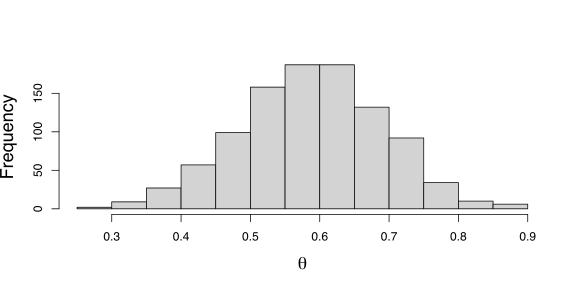
\includegraphics[width=0.75\linewidth]{IMSB_files/figure-latex/sampling1-1} 

}

\caption{Blah blah...}\label{fig:sampling1}
\end{figure}

La précision dépend de la taille de l'échantillon\ldots{}

\begin{figure}[!htb]

{\centering \includegraphics[width=0.75\linewidth]{IMSB_files/figure-latex/sampling2-1} 

}

\caption{Blah blah...}\label{fig:sampling2}
\end{figure}

\begin{figure}[!htb]

{\centering \includegraphics[width=0.75\linewidth]{IMSB_files/figure-latex/sampling3-1} 

}

\caption{Blah blah...}\label{fig:sampling3}
\end{figure}

\hypertarget{la-distribution-postuxe9rieure-ruxe9sumuxe9}{%
\subsection{La distribution postérieure, résumé}\label{la-distribution-postuxe9rieure-ruxe9sumuxe9}}

\begin{itemize}
\tightlist
\item
  Cas analytique :
\end{itemize}

\begin{Shaded}
\begin{Highlighting}[]
\NormalTok{p\_grid }\OtherTok{\textless{}{-}} \FunctionTok{seq}\NormalTok{(}\AttributeTok{from =} \DecValTok{0}\NormalTok{, }\AttributeTok{to =} \DecValTok{1}\NormalTok{, }\AttributeTok{length.out =} \DecValTok{1000}\NormalTok{)}
\NormalTok{a }\OtherTok{\textless{}{-}}\NormalTok{ b }\OtherTok{\textless{}{-}} \DecValTok{1} \CommentTok{\# parameters of the Beta prior}
\NormalTok{n }\OtherTok{\textless{}{-}} \DecValTok{9} \CommentTok{\# number of observations}
\NormalTok{y }\OtherTok{\textless{}{-}} \DecValTok{6} \CommentTok{\# number of successes}
\NormalTok{posterior }\OtherTok{\textless{}{-}} \FunctionTok{dbeta}\NormalTok{(p\_grid, z }\SpecialCharTok{+}\NormalTok{ a }\SpecialCharTok{{-}} \DecValTok{1}\NormalTok{, N }\SpecialCharTok{{-}}\NormalTok{ z }\SpecialCharTok{+}\NormalTok{ b }\SpecialCharTok{{-}} \DecValTok{1}\NormalTok{)}
\end{Highlighting}
\end{Shaded}

\begin{itemize}
\tightlist
\item
  Grid method :
\end{itemize}

\begin{Shaded}
\begin{Highlighting}[]
\NormalTok{p\_grid }\OtherTok{\textless{}{-}} \FunctionTok{seq}\NormalTok{( }\AttributeTok{from =} \DecValTok{0}\NormalTok{, }\AttributeTok{to =} \DecValTok{1}\NormalTok{, }\AttributeTok{length.out =} \DecValTok{1000}\NormalTok{)}
\NormalTok{prior }\OtherTok{\textless{}{-}} \FunctionTok{rep}\NormalTok{(}\DecValTok{1}\NormalTok{, }\DecValTok{1000}\NormalTok{) }\CommentTok{\# uniform prior}
\NormalTok{likelihood }\OtherTok{\textless{}{-}} \FunctionTok{dbinom}\NormalTok{(y, }\AttributeTok{size =}\NormalTok{ n, }\AttributeTok{prob =}\NormalTok{ p\_grid)}
\NormalTok{posterior }\OtherTok{\textless{}{-}}\NormalTok{ (likelihood }\SpecialCharTok{*}\NormalTok{ prior) }\SpecialCharTok{/} \FunctionTok{sum}\NormalTok{(likelihood }\SpecialCharTok{*}\NormalTok{ prior)}
\end{Highlighting}
\end{Shaded}

\begin{itemize}
\tightlist
\item
  Échantillonner la distribution postérieure :
\end{itemize}

\begin{Shaded}
\begin{Highlighting}[]
\FunctionTok{sample}\NormalTok{(data, }\AttributeTok{size =}\NormalTok{ trajLength, }\AttributeTok{prob =}\NormalTok{ prob, }\AttributeTok{replace =} \ConstantTok{TRUE}\NormalTok{)}
\end{Highlighting}
\end{Shaded}

\textbf{Méthode analytique}
* La distribution postérieure est décrite explicitement
* Le modèle est fortement contraint

\textbf{Méthode Grid}
* La distribution postérieure n'est donnée que pour un ensemble fini de valeurs
* Plus la grille est fine, meilleure est l'estimation de la distribution postérieure
* Compromis \emph{Précision - Temps de calcul}

\hypertarget{utiliser-les-uxe9chantillons-pour-ruxe9sumer-la-distribution-postuxe9rieure}{%
\subsection{Utiliser les échantillons pour résumer la distribution postérieure}\label{utiliser-les-uxe9chantillons-pour-ruxe9sumer-la-distribution-postuxe9rieure}}

\hypertarget{estimation-de-la-tendance-centrale}{%
\subsubsection{Estimation de la tendance centrale}\label{estimation-de-la-tendance-centrale}}

À partir d'un ensemble d'échantillons d'une distribution postérieure, on peut calculer la moyenne, le mode, et la médiane. Par exemple pour un prior uniforme, 10 lancers et 3 Faces.

\begin{Shaded}
\begin{Highlighting}[]
\NormalTok{mode\_posterior }\OtherTok{\textless{}{-}} \FunctionTok{find\_mode}\NormalTok{(samples) }\CommentTok{\# in blue}
\NormalTok{mean\_posterior }\OtherTok{\textless{}{-}} \FunctionTok{mean}\NormalTok{(samples) }\CommentTok{\# in orange}
\NormalTok{median\_posterior }\OtherTok{\textless{}{-}} \FunctionTok{median}\NormalTok{(samples) }\CommentTok{\# in green}
\end{Highlighting}
\end{Shaded}

\begin{figure}[!htb]

{\centering \includegraphics[width=0.75\linewidth]{IMSB_files/figure-latex/tendance-centrale2-1} 

}

\caption{Blah blah...}\label{fig:tendance-centrale2}
\end{figure}

Quelle est la probabilité que le biais de la pièce \(\theta\) soit supérieur à 0.5 ?

\begin{Shaded}
\begin{Highlighting}[]
\FunctionTok{sum}\NormalTok{(samples }\SpecialCharTok{\textgreater{}} \FloatTok{0.5}\NormalTok{) }\SpecialCharTok{/} \FunctionTok{length}\NormalTok{(samples) }\CommentTok{\# length(samples) is the number of samples}
\end{Highlighting}
\end{Shaded}

\begin{verbatim}
## [1] 0.112
\end{verbatim}

Quelle est la probabilité que le biais de la pièce \(\theta\) soit compris entre 0.2 et 0.4 ?

\begin{Shaded}
\begin{Highlighting}[]
\FunctionTok{sum}\NormalTok{(samples }\SpecialCharTok{\textgreater{}} \FloatTok{0.2} \SpecialCharTok{\&}\NormalTok{ samples }\SpecialCharTok{\textless{}} \FloatTok{0.4}\NormalTok{) }\SpecialCharTok{/} \FloatTok{1e4} \CommentTok{\# length(samples) is the number of samples}
\end{Highlighting}
\end{Shaded}

\begin{verbatim}
## [1] 0.5482
\end{verbatim}

\begin{figure}[!htb]

{\centering \includegraphics[width=0.75\linewidth]{IMSB_files/figure-latex/interval-prob-plot-1} 

}

\caption{Blah blah...}\label{fig:interval-prob-plot}
\end{figure}

\hypertarget{highest-density-interval-hdi}{%
\subsection{Highest density interval (HDI)}\label{highest-density-interval-hdi}}

\begin{itemize}
\tightlist
\item
  Le HDI indique les valeurs du paramètre qui sont les plus probables (sachant les données et le prior)
\item
  Plus le HDI est étroit et plus le degré de certitude est élevé
\item
  La largeur du HDI diminue avec l'augmentation du nombre de mesures
\end{itemize}

\begin{quote}
Définition: les valeurs du paramètre \(\theta\) contenues dans un HDI à 89\% sont telles que \(p(\theta) > W\) où \(W\) satisfait la condition suivante :

\[\int_{\theta \ : \ p(\theta) > W} p(\theta) \, \mathrm{d} \theta = 0.89.\]
\end{quote}

\begin{figure}[!htb]

{\centering \includegraphics[width=1\linewidth]{figures/HDI} 

}

\caption{Illustration of the Mersenne-Twister algorithm... Figure from...}\label{fig:hdi}
\end{figure}

\begin{Shaded}
\begin{Highlighting}[]
\FunctionTok{library}\NormalTok{(BEST)}

\FunctionTok{set.seed}\NormalTok{(}\DecValTok{666}\NormalTok{)}
\NormalTok{p\_grid }\OtherTok{\textless{}{-}} \FunctionTok{seq}\NormalTok{(}\AttributeTok{from =} \DecValTok{0}\NormalTok{, }\AttributeTok{to =} \DecValTok{1}\NormalTok{, }\AttributeTok{length.out =} \FloatTok{1e3}\NormalTok{)}
\NormalTok{pTheta }\OtherTok{\textless{}{-}} \FunctionTok{dbeta}\NormalTok{(p\_grid, }\DecValTok{3}\NormalTok{, }\DecValTok{10}\NormalTok{)}
\NormalTok{massVec }\OtherTok{\textless{}{-}}\NormalTok{ pTheta }\SpecialCharTok{/} \FunctionTok{sum}\NormalTok{(pTheta)}
\NormalTok{samples }\OtherTok{\textless{}{-}} \FunctionTok{sample}\NormalTok{(p\_grid, }\AttributeTok{size =} \FloatTok{1e4}\NormalTok{, }\AttributeTok{replace =} \ConstantTok{TRUE}\NormalTok{, }\AttributeTok{prob =}\NormalTok{ pTheta)}

\FunctionTok{plotPost}\NormalTok{(samples, }\AttributeTok{credMass =} \FloatTok{0.89}\NormalTok{, }\AttributeTok{cex =} \FloatTok{1.5}\NormalTok{, }\AttributeTok{xlab =} \FunctionTok{expression}\NormalTok{(theta), }\AttributeTok{xlim =} \FunctionTok{c}\NormalTok{(}\DecValTok{0}\NormalTok{, }\DecValTok{1}\NormalTok{) )}
\end{Highlighting}
\end{Shaded}

\begin{figure}[!htb]

{\centering \includegraphics[width=0.75\linewidth]{IMSB_files/figure-latex/plotpost1-1} 

}

\caption{Blah blah...}\label{fig:plotpost1}
\end{figure}

\hypertarget{region-of-practical-equivalence-rope}{%
\subsection{Region of practical equivalence (ROPE)}\label{region-of-practical-equivalence-rope}}

On l'utilise pour tester une hypothèse :

\begin{itemize}
\tightlist
\item
  La valeur du paramètre (e.g., \(\theta = 0.5\)) est rejetée si le HDI est entièrement hors de la ROPE
\item
  La valeur du paramètre (e.g., \(\theta = 0.5\)) est acceptée si le HDI est entièrement dans la ROPE
\item
  Si le HDI et la ROPE se chevauchent on ne peut pas conclure\ldots{}
\end{itemize}

\begin{figure}[!htb]

{\centering \includegraphics[width=0.75\linewidth]{IMSB_files/figure-latex/rope-1} 

}

\caption{Blah blah...}\label{fig:rope}
\end{figure}

\hypertarget{model-checking}{%
\subsection{Model checking}\label{model-checking}}

Les deux rôles de la fonction de vraisemblance :

\begin{itemize}
\tightlist
\item
  C'est une fonction de \(\theta\) pour le calcul de la distribution postérieure : \(\mathcal{L}(\theta \ | \ y, n)\)
\item
  Lorsque \(\theta\) est connu / fixé, c'est une distribution de probabilité : \(p(y \ |\ \theta, n) = \theta^y(1 - \theta)^{(n - y)}\)
\end{itemize}

On peut utiliser cette distribution de probabilité pour générer des données\ldots{} !

Par exemple : Générer 10000 valeurs à partir d'une loi binomiale basée sur 9 lancers et une probabilité de Face de 0.6 :

\begin{Shaded}
\begin{Highlighting}[]
\NormalTok{samples }\OtherTok{\textless{}{-}} \FunctionTok{rbinom}\NormalTok{(}\AttributeTok{n =} \FloatTok{1e4}\NormalTok{, }\AttributeTok{size =} \DecValTok{10}\NormalTok{, }\AttributeTok{prob =} \FloatTok{0.6}\NormalTok{)}
\end{Highlighting}
\end{Shaded}

Deux sources d'incertitude dans ces prédictions :

\begin{itemize}
\tightlist
\item
  Incertitude liée au processus d'échantillonnage
  -\textgreater{} Chaque valeur apparaît avec une probabilité \(\theta\)
\item
  Incertitude sur la valeur de \(\theta\) elle-même
  -\textgreater{} Pour chaque valeur de \(\theta\) on peut calculer une distribution implicite
\end{itemize}

Par exemple : Générer 10000 valeurs à partir d'une loi binomiale basé sur 9 lancers et une probabilité de Face décrite par la distribution postérieure de \(\theta\) :

\begin{Shaded}
\begin{Highlighting}[]
\NormalTok{samples }\OtherTok{\textless{}{-}} \FunctionTok{rbinom}\NormalTok{(}\AttributeTok{n =} \FloatTok{1e4}\NormalTok{, }\AttributeTok{size =} \DecValTok{10}\NormalTok{, }\AttributeTok{prob =} \FunctionTok{rbeta}\NormalTok{(}\FloatTok{1e4}\NormalTok{, }\DecValTok{16}\NormalTok{, }\DecValTok{10}\NormalTok{) )}
\end{Highlighting}
\end{Shaded}

\hypertarget{posterior-predictive-checking}{%
\subsection{Posterior predictive checking}\label{posterior-predictive-checking}}

\begin{figure}[!htb]

{\centering \includegraphics[width=0.75\linewidth]{IMSB_files/figure-latex/ppc-1} 

}

\caption{Blah blah...}\label{fig:ppc}
\end{figure}

Blah blah\ldots{}

\begin{figure}[!htb]

{\centering \includegraphics[width=1\linewidth]{figures/ModelPredictions} 

}

\caption{Illustration of the posterior predictive checking procedure. Figure from McElreath (2016).}\label{fig:ppc-rethinking}
\end{figure}

\hypertarget{conclusions}{%
\section{Conclusions}\label{conclusions}}

\ldots{}

\hypertarget{linear-regression1}{%
\chapter{Modèle de régression linéaire}\label{linear-regression1}}

\definecolor{steelblue}{RGB}{70, 130, 180}
\definecolor{green}{RGB}{0, 153, 0}
\definecolor{purple}{RGB}{153, 0, 153}
\definecolor{orangered}{cmyk}{0, 73, 100, 0}

Introduction au chapitre blah blah\ldots{}

\hypertarget{langage-de-la-moduxe9lisation}{%
\section{Langage de la modélisation}\label{langage-de-la-moduxe9lisation}}

\[
\begin{aligned}
y_{i} &\sim \mathrm{Normal}(\mu_{i}, \sigma) \\
\mu_{i}&= \alpha + \beta x_{i} \\
\alpha &\sim \mathrm{Normal}(60, 10) \\
\beta &\sim \mathrm{Normal}(0, 10) \\
\sigma &\sim \mathrm{HalfCauchy}(0, 1)
\end{aligned}
\]

\textbf{Objectif de la séance} : comprendre ce type de modèle.

Les constituants de nos modèles seront toujours les mêmes et nous suivrons les deux mêmes étapes :

\begin{itemize}
\tightlist
\item
  Construire le modèle (\emph{likelihood} + \emph{priors}).
\item
  Mettre à jour grâce aux données (\emph{updating}), afin de calculer la distribution postérieure.
\end{itemize}

\hypertarget{un-premier-moduxe8le}{%
\section{Un premier modèle}\label{un-premier-moduxe8le}}

\begin{Shaded}
\begin{Highlighting}[]
\FunctionTok{library}\NormalTok{(rethinking)}
\FunctionTok{library}\NormalTok{(tidyverse)}

\FunctionTok{data}\NormalTok{(Howell1)}
\NormalTok{d }\OtherTok{\textless{}{-}}\NormalTok{ Howell1}
\FunctionTok{str}\NormalTok{(d)}
\end{Highlighting}
\end{Shaded}

\begin{verbatim}
## 'data.frame':    544 obs. of  4 variables:
##  $ height: num  152 140 137 157 145 ...
##  $ weight: num  47.8 36.5 31.9 53 41.3 ...
##  $ age   : num  63 63 65 41 51 35 32 27 19 54 ...
##  $ male  : int  1 0 0 1 0 1 0 1 0 1 ...
\end{verbatim}

\begin{Shaded}
\begin{Highlighting}[]
\NormalTok{d2 }\OtherTok{\textless{}{-}}\NormalTok{ d }\SpecialCharTok{\%\textgreater{}\%} \FunctionTok{filter}\NormalTok{(age }\SpecialCharTok{\textgreater{}=} \DecValTok{18}\NormalTok{)}
\FunctionTok{head}\NormalTok{(d2)}
\end{Highlighting}
\end{Shaded}

\begin{verbatim}
##    height   weight age male
## 1 151.765 47.82561  63    1
## 2 139.700 36.48581  63    0
## 3 136.525 31.86484  65    0
## 4 156.845 53.04191  41    1
## 5 145.415 41.27687  51    0
## 6 163.830 62.99259  35    1
\end{verbatim}

\ldots{}

\[h_{i} \sim \mathrm{Normal}(\mu, \sigma)\]

\begin{Shaded}
\begin{Highlighting}[]
\NormalTok{d2 }\SpecialCharTok{\%\textgreater{}\%}
    \FunctionTok{ggplot}\NormalTok{(}\FunctionTok{aes}\NormalTok{(}\AttributeTok{x =}\NormalTok{ height) ) }\SpecialCharTok{+}
    \FunctionTok{geom\_histogram}\NormalTok{(}\AttributeTok{bins =} \DecValTok{10}\NormalTok{, }\AttributeTok{col =} \StringTok{"white"}\NormalTok{) }\SpecialCharTok{+}
    \FunctionTok{theme\_bw}\NormalTok{(}\AttributeTok{base\_size =} \DecValTok{18}\NormalTok{)}
\end{Highlighting}
\end{Shaded}

\begin{center}\includegraphics[width=0.75\linewidth]{IMSB_files/figure-latex/unnamed-chunk-13-1} \end{center}

\hypertarget{loi-normale}{%
\section{Loi normale}\label{loi-normale}}

\[
p(x \ | \ \mu, \sigma) = \frac{1}{\sqrt{2 \pi \sigma^{2}}} \exp \bigg[-\frac{1}{2 \sigma^{2}} (\mu - x)^{2} \bigg]
\]

\begin{Shaded}
\begin{Highlighting}[]
\FunctionTok{data.frame}\NormalTok{(}\AttributeTok{value =} \FunctionTok{rnorm}\NormalTok{(}\FloatTok{1e4}\NormalTok{, }\DecValTok{10}\NormalTok{, }\DecValTok{1}\NormalTok{) ) }\SpecialCharTok{\%\textgreater{}\%} \CommentTok{\# 10000 samples from Normal(10, 1)}
    \FunctionTok{ggplot}\NormalTok{(}\FunctionTok{aes}\NormalTok{(}\AttributeTok{x =}\NormalTok{ value) ) }\SpecialCharTok{+}
    \FunctionTok{geom\_histogram}\NormalTok{(}\AttributeTok{col =} \StringTok{"white"}\NormalTok{) }\SpecialCharTok{+}
    \FunctionTok{theme\_bw}\NormalTok{(}\AttributeTok{base\_size =} \DecValTok{20}\NormalTok{)}
\end{Highlighting}
\end{Shaded}

\begin{center}\includegraphics[width=0.75\linewidth]{IMSB_files/figure-latex/unnamed-chunk-14-1} \end{center}

\hypertarget{douxf9-vient-la-loi-normale}{%
\subsection{D'où vient la loi normale ?}\label{douxf9-vient-la-loi-normale}}

Certaines valeurs sont fortement probables (autour de la moyenne \(\mu\)). Plus on s'éloigne, moins les valeurs sont probables (en suivant une décroissance exponentielle).

\begin{figure}[!htb]

{\centering \includegraphics[width=0.75\linewidth]{IMSB_files/figure-latex/normal-explain1-1} 

}

\caption{blah blah...}\label{fig:normal-explain1}
\end{figure}

\[
y = \exp \big[-x^{2} \big]
\]

On étend notre fonction aux valeurs négatives.

\begin{figure}[!htb]

{\centering \includegraphics[width=0.75\linewidth]{IMSB_files/figure-latex/normal-explain2-1} 

}

\caption{blah blah...}\label{fig:normal-explain2}
\end{figure}

\[
y = \exp \big[-x^{2} \big]
\]

Les points d'inflection nous donnent une bonne indication de là où la plupart des valeurs se trouvent (i.e., entre les points d'inflection). Les pics de la dérivée nous montrent les points d'inflection.

\begin{figure}[!htb]

{\centering \includegraphics[width=0.75\linewidth]{IMSB_files/figure-latex/normal-explain3-1} 

}

\caption{blah blah...}\label{fig:normal-explain3}
\end{figure}

\[
y = \exp \bigg [- \frac{1}{2} x^{2} \bigg]
\]

Ensuite on standardise la distribution de manière à ce que les deux points d'inflection se trouvent à \(x = -1\) et \(x = 1\).

\begin{figure}[!htb]

{\centering \includegraphics[width=0.75\linewidth]{IMSB_files/figure-latex/normal-explain4-1} 

}

\caption{blah blah...}\label{fig:normal-explain4}
\end{figure}

\[
y = \exp \bigg [- \frac{1}{2 \color{steelblue}{\sigma^{2}}} x^{2} \bigg]
\]

On insère un paramètre \(\sigma^{2}\) pour contrôler la distance entre les points d'inflection.

\begin{figure}[!htb]

{\centering \includegraphics[width=0.75\linewidth]{IMSB_files/figure-latex/normal-explain5-1} 

}

\caption{blah blah...}\label{fig:normal-explain5}
\end{figure}

\[
y = \exp \bigg [- \frac{1}{2 \color{steelblue}{\sigma^{2}}} (x - \color{orangered}{\mu})^{2} \bigg]
\]

On insère ensuite un paramètre \(\mu\) afin de pouvoir contrôler la position (la tendance centrale) de la distribution.

\begin{figure}[!htb]

{\centering \includegraphics[width=0.75\linewidth]{IMSB_files/figure-latex/normal-explain6-1} 

}

\caption{blah blah...}\label{fig:normal-explain6}
\end{figure}

\[
y = \frac{1}{\sqrt{2 \pi \color{steelblue}{\sigma^{2}}}} \exp \bigg[-\frac{1}{2 \color{steelblue}{\sigma^{2}}} (\color{orangered}{\mu} - x)^{2} \bigg]
\]

Mais\ldots{} cette distribution n'intègre pas à 1. On divise donc par une constante de normalisation (la partie gauche), afin d'obtenir une distribution de probabilité.

\begin{figure}[!htb]

{\centering \includegraphics[width=0.75\linewidth]{IMSB_files/figure-latex/normal-explain7-1} 

}

\caption{blah blah...}\label{fig:normal-explain7}
\end{figure}

\hypertarget{moduxe8le-gaussien}{%
\section{Modèle gaussien}\label{moduxe8le-gaussien}}

Nous allons construire un modèle de régression, mais avant d'ajouter un prédicteur, essayons de modéliser la distribution des tailles.

On cherche à savoir quel est le modèle (la distribution) qui décrit le mieux la répartition des tailles. On va donc explorer toutes les combinaisons possibles de \(\mu\) et \(\sigma\) et les classer par leurs probabilités respectives.

Notre but, une fois encore, est de décrire \textbf{la distribution postérieure}, qui sera donc d'une certaine manière \textbf{une distribution de distributions}.

On définit ensuite \(p(\mu,\sigma)\), la distribution a priori conjointe de tous les paramètres du modèle. On peut spécifier ces priors indépendamment pour chaque paramètre, sachant que \(p(\mu, \sigma) = p(\mu) p(\sigma)\).

\[\color{steelblue}{\mu \sim \mathrm{Normal}(178,20)}\]

\begin{figure}[!htb]

{\centering \includegraphics[width=0.75\linewidth]{IMSB_files/figure-latex/unnamed-chunk-15-1} 

}

\caption{blah blah...}\label{fig:unnamed-chunk-15}
\end{figure}

On définit ensuite \(p(\mu,\sigma)\), la distribution a priori conjointe de tous les paramètres du modèle. On peut spécifier ces priors indépendamment pour chaque paramètre, sachant que \(p(\mu, \sigma) = p(\mu) p(\sigma)\).

\[\color{steelblue}{\sigma \sim \mathrm{Uniform}(0,50)}\]

\begin{figure}[!htb]

{\centering \includegraphics[width=0.75\linewidth]{IMSB_files/figure-latex/plot-prior1-1} 

}

\caption{blah blah...}\label{fig:plot-prior1}
\end{figure}

\hypertarget{visualiser-le-prior}{%
\section{Visualiser le prior}\label{visualiser-le-prior}}

\begin{Shaded}
\begin{Highlighting}[]
\FunctionTok{library}\NormalTok{(ks)}
\NormalTok{sample\_mu }\OtherTok{\textless{}{-}} \FunctionTok{rnorm}\NormalTok{(}\FloatTok{1e4}\NormalTok{, }\DecValTok{178}\NormalTok{, }\DecValTok{20}\NormalTok{) }\CommentTok{\# prior on mu}
\NormalTok{sample\_sigma }\OtherTok{\textless{}{-}} \FunctionTok{runif}\NormalTok{(}\FloatTok{1e4}\NormalTok{, }\DecValTok{0}\NormalTok{, }\DecValTok{50}\NormalTok{) }\CommentTok{\# prior on sigma}
\NormalTok{prior }\OtherTok{\textless{}{-}} \FunctionTok{data.frame}\NormalTok{(}\FunctionTok{cbind}\NormalTok{(sample\_mu, sample\_sigma) ) }\CommentTok{\# multivariate prior}
\NormalTok{H.scv }\OtherTok{\textless{}{-}} \FunctionTok{Hscv}\NormalTok{(}\AttributeTok{x =}\NormalTok{ prior, }\AttributeTok{verbose =} \ConstantTok{TRUE}\NormalTok{)}
\NormalTok{fhat\_prior }\OtherTok{\textless{}{-}} \FunctionTok{kde}\NormalTok{(}\AttributeTok{x =}\NormalTok{ prior, }\AttributeTok{H =}\NormalTok{ H.scv, }\AttributeTok{compute.cont =} \ConstantTok{TRUE}\NormalTok{)}
\FunctionTok{plot}\NormalTok{(}
\NormalTok{    fhat\_prior, }\AttributeTok{display =} \StringTok{"persp"}\NormalTok{, }\AttributeTok{col =} \StringTok{"steelblue"}\NormalTok{, }\AttributeTok{border =} \ConstantTok{NA}\NormalTok{,}
    \AttributeTok{xlab =} \StringTok{"}\SpecialCharTok{\textbackslash{}n}\StringTok{mu"}\NormalTok{, }\AttributeTok{ylab =} \StringTok{"}\SpecialCharTok{\textbackslash{}n}\StringTok{sigma"}\NormalTok{, }\AttributeTok{zlab =} \StringTok{"}\SpecialCharTok{\textbackslash{}n\textbackslash{}n}\StringTok{p(mu, sigma)"}\NormalTok{,}
    \AttributeTok{shade =} \FloatTok{0.8}\NormalTok{, }\AttributeTok{phi =} \DecValTok{30}\NormalTok{, }\AttributeTok{ticktype =} \StringTok{"detailed"}\NormalTok{,}
    \AttributeTok{cex.lab =} \FloatTok{1.2}\NormalTok{, }\AttributeTok{family =} \StringTok{"Helvetica"}\NormalTok{)}
\end{Highlighting}
\end{Shaded}

\begin{Shaded}
\begin{Highlighting}[]
\NormalTok{knitr}\SpecialCharTok{::}\FunctionTok{include\_graphics}\NormalTok{(}\StringTok{"figures/prior.png"}\NormalTok{)}
\end{Highlighting}
\end{Shaded}

\begin{figure}[!htb]

{\centering \includegraphics[width=0.75\linewidth]{figures/prior} 

}

\caption{blah blah...}\label{fig:plot-prior-2d-knitr}
\end{figure}

\hypertarget{uxe9chantillonner-uxe0-partir-du-prior}{%
\section{Échantillonner à partir du prior}\label{uxe9chantillonner-uxe0-partir-du-prior}}

\begin{Shaded}
\begin{Highlighting}[]
\NormalTok{sample\_mu }\OtherTok{\textless{}{-}} \FunctionTok{rnorm}\NormalTok{(}\DecValTok{1000}\NormalTok{, }\DecValTok{178}\NormalTok{, }\DecValTok{20}\NormalTok{)}
\NormalTok{sample\_sigma }\OtherTok{\textless{}{-}} \FunctionTok{runif}\NormalTok{(}\DecValTok{1000}\NormalTok{, }\DecValTok{0}\NormalTok{, }\DecValTok{50}\NormalTok{)}

\FunctionTok{data.frame}\NormalTok{(}\AttributeTok{x =} \FunctionTok{rnorm}\NormalTok{(}\DecValTok{1000}\NormalTok{, sample\_mu, sample\_sigma) ) }\SpecialCharTok{\%\textgreater{}\%}
    \FunctionTok{ggplot}\NormalTok{(}\FunctionTok{aes}\NormalTok{(x) ) }\SpecialCharTok{+}
    \FunctionTok{geom\_histogram}\NormalTok{() }\SpecialCharTok{+}
    \FunctionTok{xlab}\NormalTok{(}\FunctionTok{expression}\NormalTok{(y[i]) ) }\SpecialCharTok{+}
    \FunctionTok{theme\_bw}\NormalTok{(}\AttributeTok{base\_size =} \DecValTok{20}\NormalTok{)}
\end{Highlighting}
\end{Shaded}

\begin{figure}[!htb]

{\centering \includegraphics[width=0.75\linewidth]{IMSB_files/figure-latex/plot-prior-sigma-1} 

}

\caption{blah blah...}\label{fig:plot-prior-sigma}
\end{figure}

\hypertarget{fonction-de-vraisemblance}{%
\section{Fonction de vraisemblance}\label{fonction-de-vraisemblance}}

\begin{Shaded}
\begin{Highlighting}[]
\NormalTok{mu\_exemple }\OtherTok{\textless{}{-}} \FloatTok{151.23}
\NormalTok{sigma\_exemple }\OtherTok{\textless{}{-}} \FloatTok{23.42}

\NormalTok{d2}\SpecialCharTok{$}\NormalTok{height[}\DecValTok{34}\NormalTok{] }\CommentTok{\# one observation}
\end{Highlighting}
\end{Shaded}

\begin{verbatim}
## [1] 162.8648
\end{verbatim}

\begin{figure}[!htb]

{\centering \includegraphics[width=0.75\linewidth]{IMSB_files/figure-latex/likelihood-plot-1} 

}

\caption{blah blah...}\label{fig:likelihood-plot}
\end{figure}

On veut calculer la probabilité d'observer une certaine valeur de taille, sachant certaines valeurs de \(\mu\) et \(\sigma\), c'est à dire :

\[
p(x \ | \ \mu, \sigma) = \frac{1}{\sqrt{2 \pi \sigma^{2}}} \exp \bigg[-\frac{1}{2 \sigma^{2}} (\mu - x)^{2} \bigg]
\]

On peut calculer cette \emph{densité de probabilité} à l'aide des fonctions \texttt{dnorm}, \texttt{dbeta}, \texttt{dt}, \texttt{dexp}, \texttt{dgamma}, etc.

\begin{Shaded}
\begin{Highlighting}[]
\FunctionTok{dnorm}\NormalTok{(d2}\SpecialCharTok{$}\NormalTok{height[}\DecValTok{34}\NormalTok{], mu\_exemple, sigma\_exemple)}
\end{Highlighting}
\end{Shaded}

\begin{verbatim}
## [1] 0.01505675
\end{verbatim}

\[
p(x \ | \ \mu, \sigma) = \frac{1}{\sqrt{2 \pi \sigma^{2}}} \exp \bigg[-\frac{1}{2 \sigma^{2}} (\mu - x)^{2} \bigg]
\]

Ou à la main\ldots{}

\begin{Shaded}
\begin{Highlighting}[]
\NormalTok{normal\_likelihood }\OtherTok{\textless{}{-}} \ControlFlowTok{function}\NormalTok{ (x, mu, sigma) \{}
  
\NormalTok{  bell }\OtherTok{\textless{}{-}} \FunctionTok{exp}\NormalTok{( (}\SpecialCharTok{{-}} \DecValTok{1} \SpecialCharTok{/}\NormalTok{ (}\DecValTok{2} \SpecialCharTok{*}\NormalTok{ sigma}\SpecialCharTok{\^{}}\DecValTok{2}\NormalTok{) ) }\SpecialCharTok{*}\NormalTok{ (mu }\SpecialCharTok{{-}}\NormalTok{ x)}\SpecialCharTok{\^{}}\DecValTok{2}\NormalTok{ )}
\NormalTok{  norm }\OtherTok{\textless{}{-}} \FunctionTok{sqrt}\NormalTok{(}\DecValTok{2} \SpecialCharTok{*}\NormalTok{ pi }\SpecialCharTok{*}\NormalTok{ sigma}\SpecialCharTok{\^{}}\DecValTok{2}\NormalTok{)}
  
  \FunctionTok{return}\NormalTok{(bell }\SpecialCharTok{/}\NormalTok{ norm)}
  
\NormalTok{\}}
\end{Highlighting}
\end{Shaded}

\begin{Shaded}
\begin{Highlighting}[]
\FunctionTok{normal\_likelihood}\NormalTok{(d2}\SpecialCharTok{$}\NormalTok{height[}\DecValTok{34}\NormalTok{], mu\_exemple, sigma\_exemple)}
\end{Highlighting}
\end{Shaded}

\begin{verbatim}
## [1] 0.01505675
\end{verbatim}

\hypertarget{distribution-postuxe9rieure}{%
\section{Distribution postérieure}\label{distribution-postuxe9rieure}}

\[
\color{purple}{p(\mu, \sigma \ | \ h)} = \frac{\prod_{i} \color{orangered}{\mathrm{Normal}(h_{i} \ | \ \mu, \sigma)}\color{steelblue}{\mathrm{Normal}(\mu \ | \ 178, 20)\mathrm{Uniform}(\sigma \ | \ 0, 50)}}
{\color{green}{\int \int \prod_{i} \mathrm{Normal}(h_{i} \ | \ \mu, \sigma)\mathrm{Normal}(\mu \ | \ 178, 20)\mathrm{Uniform}(\sigma \ | \ 0, 50) \mathrm{d} \mu \mathrm{d} \sigma}}
\]

\[
\color{purple}{p(\mu, \sigma \ | \ h)} \propto \prod_{i} \color{orangered}{\mathrm{Normal}(h_{i} \ | \ \mu, \sigma)}\color{steelblue}{\mathrm{Normal}(\mu \ | \ 178, 20)\mathrm{Uniform}(\sigma \ | \ 0, 50)}
\]

Il s'agit de la même formule vue lors des cours 1 et 2, mais cette fois en considérant qu'il existe plusieurs observations de taille (\(h_{i}\)), et deux paramètres à estimer \(\mu\) et \(\sigma\).

Pour calculer la \textbf{vraisemblance marginale} (en vert), il faut donc intégrer sur deux paramètres : \(\mu\) et \(\sigma\).

On réalise ici encore que la probabilité a posteriori est proportionnelle au produit de la vraisemblance et du prior.

\hypertarget{distribution-postuxe9rieure---grid-approximation}{%
\subsection{Distribution postérieure - grid approximation}\label{distribution-postuxe9rieure---grid-approximation}}

\begin{Shaded}
\begin{Highlighting}[]
\CommentTok{\# définit une grille de valeurs possibles pour mu et sigma}
\NormalTok{mu.list }\OtherTok{\textless{}{-}} \FunctionTok{seq}\NormalTok{(}\AttributeTok{from =} \DecValTok{140}\NormalTok{, }\AttributeTok{to =} \DecValTok{160}\NormalTok{, }\AttributeTok{length.out =} \DecValTok{200}\NormalTok{)}
\NormalTok{sigma.list }\OtherTok{\textless{}{-}} \FunctionTok{seq}\NormalTok{(}\AttributeTok{from =} \DecValTok{4}\NormalTok{, }\AttributeTok{to =} \DecValTok{9}\NormalTok{, }\AttributeTok{length.out =} \DecValTok{200}\NormalTok{)}

\CommentTok{\# étend la grille en deux dimensions (chaque combinaison de mu et sigma)}
\NormalTok{post }\OtherTok{\textless{}{-}} \FunctionTok{expand.grid}\NormalTok{(}\AttributeTok{mu =}\NormalTok{ mu.list, }\AttributeTok{sigma =}\NormalTok{ sigma.list)}

\CommentTok{\# calcul de la log{-}vraisemblance (pour chaque couple de mu et sigma)}
\NormalTok{post}\SpecialCharTok{$}\NormalTok{LL }\OtherTok{\textless{}{-}}
  \FunctionTok{sapply}\NormalTok{(}
    \DecValTok{1}\SpecialCharTok{:}\FunctionTok{nrow}\NormalTok{(post),}
    \ControlFlowTok{function}\NormalTok{(i) }\FunctionTok{sum}\NormalTok{(}\FunctionTok{dnorm}\NormalTok{(}
\NormalTok{      d2}\SpecialCharTok{$}\NormalTok{height,}
      \AttributeTok{mean =}\NormalTok{ post}\SpecialCharTok{$}\NormalTok{mu[i],}
      \AttributeTok{sd =}\NormalTok{ post}\SpecialCharTok{$}\NormalTok{sigma[i],}
      \AttributeTok{log =} \ConstantTok{TRUE}\NormalTok{)}
\NormalTok{      )}
\NormalTok{    )}

\CommentTok{\# calcul de la probabilité a posteriori (non normalisée)}
\NormalTok{post}\SpecialCharTok{$}\NormalTok{prod }\OtherTok{\textless{}{-}}
\NormalTok{  post}\SpecialCharTok{$}\NormalTok{LL }\SpecialCharTok{+}
  \FunctionTok{dnorm}\NormalTok{(post}\SpecialCharTok{$}\NormalTok{mu, }\DecValTok{178}\NormalTok{, }\DecValTok{20}\NormalTok{, }\AttributeTok{log =} \ConstantTok{TRUE}\NormalTok{) }\SpecialCharTok{+}
  \FunctionTok{dunif}\NormalTok{(post}\SpecialCharTok{$}\NormalTok{sigma, }\DecValTok{0}\NormalTok{, }\DecValTok{50}\NormalTok{, }\AttributeTok{log =} \ConstantTok{TRUE}\NormalTok{)}

\CommentTok{\# on "annule" le log en avec exp() et on standardise par la valeur maximale}
\NormalTok{post}\SpecialCharTok{$}\NormalTok{prob }\OtherTok{\textless{}{-}} \FunctionTok{exp}\NormalTok{(post}\SpecialCharTok{$}\NormalTok{prod }\SpecialCharTok{{-}} \FunctionTok{max}\NormalTok{(post}\SpecialCharTok{$}\NormalTok{prod) )}
\end{Highlighting}
\end{Shaded}

\begin{Shaded}
\begin{Highlighting}[]
\NormalTok{sample.rows }\OtherTok{\textless{}{-}} \FunctionTok{sample}\NormalTok{(}\DecValTok{1}\SpecialCharTok{:}\FunctionTok{nrow}\NormalTok{(post), }\AttributeTok{size =} \FloatTok{1e4}\NormalTok{, }\AttributeTok{replace =} \ConstantTok{TRUE}\NormalTok{, }\AttributeTok{prob =}\NormalTok{ post}\SpecialCharTok{$}\NormalTok{prob)}
\end{Highlighting}
\end{Shaded}

\begin{figure}[!htb]

{\centering \includegraphics[width=0.75\linewidth]{IMSB_files/figure-latex/plotting-samples-1} 

}

\caption{blah blah...}\label{fig:plotting-samples}
\end{figure}

\hypertarget{distribution-postuxe9rieure---distributions-marginales}{%
\subsection{Distribution postérieure - distributions marginales}\label{distribution-postuxe9rieure---distributions-marginales}}

\begin{Shaded}
\begin{Highlighting}[]
\NormalTok{BEST}\SpecialCharTok{::}\FunctionTok{plotPost}\NormalTok{(}
\NormalTok{  sample.mu, }\AttributeTok{breaks =} \DecValTok{40}\NormalTok{, }\AttributeTok{xlab =} \FunctionTok{expression}\NormalTok{(mu)}
\NormalTok{  )}
\end{Highlighting}
\end{Shaded}

\begin{figure}[!htb]

{\centering \includegraphics[width=0.75\linewidth]{IMSB_files/figure-latex/unnamed-chunk-20-1} 

}

\caption{blah blah...}\label{fig:unnamed-chunk-20}
\end{figure}

\begin{Shaded}
\begin{Highlighting}[]
\NormalTok{BEST}\SpecialCharTok{::}\FunctionTok{plotPost}\NormalTok{(}
\NormalTok{  sample.sigma, }\AttributeTok{breaks =} \DecValTok{40}\NormalTok{, }\AttributeTok{xlab =} \FunctionTok{expression}\NormalTok{(sigma)}
\NormalTok{  )}
\end{Highlighting}
\end{Shaded}

\begin{figure}[!htb]

{\centering \includegraphics[width=0.75\linewidth]{IMSB_files/figure-latex/unnamed-chunk-21-1} 

}

\caption{blah blah...}\label{fig:unnamed-chunk-21}
\end{figure}

\hypertarget{introduction-uxe0-brms}{%
\section{Introduction à brms}\label{introduction-uxe0-brms}}

Under the hood : \texttt{Stan} est un langage de programmation probabiliste écrit en \texttt{C++}, et qui implémente plusieurs algorithmes de MCMC: HMC, NUTS, L-BFGS\ldots{}

\begin{Shaded}
\begin{Highlighting}[]
\NormalTok{data \{}
\NormalTok{  int}\SpecialCharTok{\textless{}}\NormalTok{lower}\OtherTok{=}\DecValTok{0}\SpecialCharTok{\textgreater{}}\NormalTok{ J; }\SpecialCharTok{/}\ErrorTok{/}\NormalTok{ number of schools }
\NormalTok{  real y[J]; }\SpecialCharTok{/}\ErrorTok{/}\NormalTok{ estimated treatment effects}
\NormalTok{  real}\SpecialCharTok{\textless{}}\NormalTok{lower}\OtherTok{=}\DecValTok{0}\SpecialCharTok{\textgreater{}}\NormalTok{ sigma[J]; }\SpecialCharTok{/}\ErrorTok{/}\NormalTok{ s.e. of effect estimates }
\NormalTok{\}}

\NormalTok{parameters \{}
\NormalTok{  real mu; }
\NormalTok{  real}\SpecialCharTok{\textless{}}\NormalTok{lower}\OtherTok{=}\DecValTok{0}\SpecialCharTok{\textgreater{}}\NormalTok{ tau;}
\NormalTok{  real eta[J];}
\NormalTok{\}}

\NormalTok{transformed parameters \{}
\NormalTok{  real theta[J];}
  \ControlFlowTok{for}\NormalTok{ (j }\ControlFlowTok{in} \DecValTok{1}\SpecialCharTok{:}\NormalTok{J)}
\NormalTok{    theta[j] }\OtherTok{=}\NormalTok{ mu }\SpecialCharTok{+}\NormalTok{ tau }\SpecialCharTok{*}\NormalTok{ eta[j];}
\NormalTok{\}}

\NormalTok{model \{}
\NormalTok{  target }\SpecialCharTok{+}\ErrorTok{=} \FunctionTok{normal\_lpdf}\NormalTok{(eta }\SpecialCharTok{|} \DecValTok{0}\NormalTok{, }\DecValTok{1}\NormalTok{);}
\NormalTok{  target }\SpecialCharTok{+}\ErrorTok{=} \FunctionTok{normal\_lpdf}\NormalTok{(y }\SpecialCharTok{|}\NormalTok{ theta, sigma);}
\NormalTok{\}}
\end{Highlighting}
\end{Shaded}

Le package \texttt{brms} (\href{https://www.jstatsoft.org/article/view/v080i01}{Bürkner, 2017}) permet de fitter des modèles multi-niveaux (ou pas) linéaires (ou pas) bayésiens en \texttt{Stan} mais en utilisant la syntaxe de \texttt{lme4}.

Par exemple, le modèle suivant :

\[
\begin{aligned}
y_{i} &\sim \mathrm{Normal}(\mu_{i}, \sigma) \\
\mu_{i} &= \alpha + \alpha_{subject[i]} + \alpha_{item[i]} + \beta x_{i} \\
\end{aligned}
\]

se spécifie avec \texttt{brms} (comme avec \texttt{lme4}) de la manière suivante :

\begin{Shaded}
\begin{Highlighting}[]
\FunctionTok{brm}\NormalTok{(y }\SpecialCharTok{\textasciitilde{}}\NormalTok{ x }\SpecialCharTok{+}\NormalTok{ (}\DecValTok{1} \SpecialCharTok{|}\NormalTok{ subject) }\SpecialCharTok{+}\NormalTok{ (}\DecValTok{1} \SpecialCharTok{|}\NormalTok{ item), }\AttributeTok{data =}\NormalTok{ d, }\AttributeTok{family =} \FunctionTok{gaussian}\NormalTok{() )}
\end{Highlighting}
\end{Shaded}

\hypertarget{rappels-de-syntaxe}{%
\subsection{Rappels de syntaxe}\label{rappels-de-syntaxe}}

Le package \texttt{brms} utilise la même syntaxe que les fonctions de base R (comme \texttt{lm}) ou que le package \texttt{lme4}.

\begin{Shaded}
\begin{Highlighting}[]
\NormalTok{Reaction }\SpecialCharTok{\textasciitilde{}}\NormalTok{ Days }\SpecialCharTok{+}\NormalTok{ (}\DecValTok{1} \SpecialCharTok{+}\NormalTok{ Days }\SpecialCharTok{|}\NormalTok{ Subject)}
\end{Highlighting}
\end{Shaded}

La partie gauche représente notre variable dépendante (ou \emph{outcome}, i.e., ce qu'on essaye de prédire). Le package \texttt{brms} permet également de fitter des modèles multivariés (plusieurs outcomes) en les combinant avec \texttt{mvbind()}:

\begin{Shaded}
\begin{Highlighting}[]
\FunctionTok{mvbind}\NormalTok{(Reaction, Memory) }\SpecialCharTok{\textasciitilde{}}\NormalTok{ Days }\SpecialCharTok{+}\NormalTok{ (}\DecValTok{1} \SpecialCharTok{+}\NormalTok{ Days }\SpecialCharTok{|}\NormalTok{ Subject)}
\end{Highlighting}
\end{Shaded}

La partie droite permet de définir les prédicteurs. L'intercept est généralement implicite, de sorte que les deux écritures ci-dessous sont équivalentes.

\begin{Shaded}
\begin{Highlighting}[]
\FunctionTok{mvbind}\NormalTok{(Reaction, Memory) }\SpecialCharTok{\textasciitilde{}}\NormalTok{ Days }\SpecialCharTok{+}\NormalTok{ (}\DecValTok{1} \SpecialCharTok{+}\NormalTok{ Days }\SpecialCharTok{|}\NormalTok{ Subject)}
\FunctionTok{mvbind}\NormalTok{(Reaction, Memory) }\SpecialCharTok{\textasciitilde{}} \DecValTok{1} \SpecialCharTok{+}\NormalTok{ Days }\SpecialCharTok{+}\NormalTok{ (}\DecValTok{1} \SpecialCharTok{+}\NormalTok{ Days }\SpecialCharTok{|}\NormalTok{ Subject)}
\end{Highlighting}
\end{Shaded}

Si l'on veut fitter un modèle sans intercept (why not), il faut le spécifier explicitement comme ci-dessous.

\begin{Shaded}
\begin{Highlighting}[]
\FunctionTok{mvbind}\NormalTok{(Reaction, Memory) }\SpecialCharTok{\textasciitilde{}} \DecValTok{0} \SpecialCharTok{+}\NormalTok{ Days }\SpecialCharTok{+}\NormalTok{ (}\DecValTok{1} \SpecialCharTok{+}\NormalTok{ Days }\SpecialCharTok{|}\NormalTok{ Subject)}
\end{Highlighting}
\end{Shaded}

Par défaut \texttt{brms} postule une vraisemblance gaussienne. Ce postulat peut être changé facilement en spécifiant la vraisemblance souhaitée via l'argument \texttt{family}.

\begin{Shaded}
\begin{Highlighting}[]
\FunctionTok{brm}\NormalTok{(Reaction }\SpecialCharTok{\textasciitilde{}} \DecValTok{1} \SpecialCharTok{+}\NormalTok{ Days }\SpecialCharTok{+}\NormalTok{ (}\DecValTok{1} \SpecialCharTok{+}\NormalTok{ Days }\SpecialCharTok{|}\NormalTok{ Subject), }\AttributeTok{family =} \FunctionTok{lognormal}\NormalTok{() )}
\end{Highlighting}
\end{Shaded}

Lisez la documentation (c'est très enthousiasmant à lire) accessible via \texttt{?brm}.

\hypertarget{quelques-fonctions-utiles}{%
\subsection{Quelques fonctions utiles}\label{quelques-fonctions-utiles}}

\begin{Shaded}
\begin{Highlighting}[]
\CommentTok{\# Generate the Stan code:}
\FunctionTok{make\_stancode}\NormalTok{(formula, ...)}
\FunctionTok{stancode}\NormalTok{(fit)}

\CommentTok{\# Generate the data passed to Stan:}
\FunctionTok{make\_standata}\NormalTok{(formula, ...)}
\FunctionTok{standata}\NormalTok{(fit)}

\CommentTok{\# Handle priors:}
\FunctionTok{get\_prior}\NormalTok{(formula, ...)}
\FunctionTok{set\_prior}\NormalTok{(prior, ...)}

\CommentTok{\# Generate expected values and predictions:}
\FunctionTok{fitted}\NormalTok{(fit, ...)}
\FunctionTok{predict}\NormalTok{(fit, ...)}
\FunctionTok{marginal\_effects}\NormalTok{(fit, ...)}

\CommentTok{\# Model comparison:}
\FunctionTok{loo}\NormalTok{(fit1, fit2, ...)}
\FunctionTok{bayes\_factor}\NormalTok{(fit1, fit2, ...)}
\FunctionTok{model\_weights}\NormalTok{(fit1, fit2, ...)}

\CommentTok{\# Hypothesis testing:}
\FunctionTok{hypothesis}\NormalTok{(fit, hypothesis, ...)}
\end{Highlighting}
\end{Shaded}

\hypertarget{un-premier-exemple}{%
\subsection{Un premier exemple}\label{un-premier-exemple}}

\begin{Shaded}
\begin{Highlighting}[]
\FunctionTok{library}\NormalTok{(brms)}
\NormalTok{mod1 }\OtherTok{\textless{}{-}} \FunctionTok{brm}\NormalTok{(height }\SpecialCharTok{\textasciitilde{}} \DecValTok{1}\NormalTok{, }\AttributeTok{data =}\NormalTok{ d2)}
\end{Highlighting}
\end{Shaded}

\begin{Shaded}
\begin{Highlighting}[]
\FunctionTok{rbind}\NormalTok{(}\FunctionTok{summary}\NormalTok{(mod1)}\SpecialCharTok{$}\NormalTok{fixed, }\FunctionTok{summary}\NormalTok{(mod1)}\SpecialCharTok{$}\NormalTok{spec\_pars )}
\end{Highlighting}
\end{Shaded}

\begin{verbatim}
##             Estimate Est.Error   l-95% CI   u-95% CI     Rhat Bulk_ESS Tail_ESS
## Intercept 154.599646 0.4264638 153.758096 155.447157 1.001954 3354.586 2603.114
## sigma       7.759921 0.2968472   7.221742   8.365626 1.000931 3661.881 2319.010
\end{verbatim}

Ces données représentent les distributions marginales de chaque paramètre. En d'autres termes, la \emph{probabilité} de chaque valeur de \(\mu\), après avoir \emph{moyenné} sur toutes les valeurs possible de \(\sigma\), est décrite par une distribution gaussienne avec une moyenne de \(154.61\) et un écart type de \(0.41\). L'intervalle de crédibilité (\(\neq\) intervalle de confiance) nous indique les 95\% valeurs de \(\mu\) ou \(\sigma\) les plus probables (sachant les données et les priors).

\hypertarget{en-utilisant-notre-prior}{%
\subsection{En utilisant notre prior}\label{en-utilisant-notre-prior}}

Par défaut \texttt{brms} utilise un prior très peu informatif centré sur la valeur moyenne de la variable mesurée. On peut donc affiner l'estimation réalisée par ce modèle en utilisant nos connaissances sur la distribution habituelle des tailles chez les humains.

La fonction \texttt{get\_prior()} permet de visualiser une liste des priors par défaut ainsi que de tous les prios qu'on peut spécifier, sachant une certaine formule (i.e., une manière d'écrire notre modèle) et un jeu de données.

\begin{Shaded}
\begin{Highlighting}[]
\FunctionTok{get\_prior}\NormalTok{(height }\SpecialCharTok{\textasciitilde{}} \DecValTok{1}\NormalTok{, }\AttributeTok{data =}\NormalTok{ d2)}
\end{Highlighting}
\end{Shaded}

\begin{verbatim}
##                     prior     class coef group resp dpar nlpar lb ub  source
##  student_t(3, 154.3, 8.5) Intercept                                  default
##      student_t(3, 0, 8.5)     sigma                             0    default
\end{verbatim}

\ldots{}

\begin{Shaded}
\begin{Highlighting}[]
\NormalTok{priors }\OtherTok{\textless{}{-}} \FunctionTok{c}\NormalTok{(}
  \FunctionTok{prior}\NormalTok{(}\FunctionTok{normal}\NormalTok{(}\DecValTok{178}\NormalTok{, }\DecValTok{20}\NormalTok{), }\AttributeTok{class =}\NormalTok{ Intercept),}
  \FunctionTok{prior}\NormalTok{(}\FunctionTok{exponential}\NormalTok{(}\FloatTok{0.01}\NormalTok{), }\AttributeTok{class =}\NormalTok{ sigma)}
\NormalTok{  )}

\NormalTok{mod2 }\OtherTok{\textless{}{-}} \FunctionTok{brm}\NormalTok{(}
\NormalTok{  height }\SpecialCharTok{\textasciitilde{}} \DecValTok{1}\NormalTok{,}
  \AttributeTok{prior =}\NormalTok{ priors,}
  \AttributeTok{family =} \FunctionTok{gaussian}\NormalTok{(),}
  \AttributeTok{data =}\NormalTok{ d2}
\NormalTok{  )}
\end{Highlighting}
\end{Shaded}

\begin{figure}[!htb]

{\centering \includegraphics[width=0.75\linewidth]{IMSB_files/figure-latex/prior-mod2-1} 

}

\caption{blah blah...}\label{fig:prior-mod2}
\end{figure}

\ldots{}

\begin{Shaded}
\begin{Highlighting}[]
\FunctionTok{summary}\NormalTok{(mod2)}
\end{Highlighting}
\end{Shaded}

\begin{verbatim}
##  Family: gaussian 
##   Links: mu = identity; sigma = identity 
## Formula: height ~ 1 
##    Data: d2 (Number of observations: 352) 
##   Draws: 4 chains, each with iter = 2000; warmup = 1000; thin = 1;
##          total post-warmup draws = 4000
## 
## Population-Level Effects: 
##           Estimate Est.Error l-95% CI u-95% CI Rhat Bulk_ESS Tail_ESS
## Intercept   154.60      0.41   153.78   155.40 1.00     2902     2067
## 
## Family Specific Parameters: 
##       Estimate Est.Error l-95% CI u-95% CI Rhat Bulk_ESS Tail_ESS
## sigma     7.77      0.29     7.23     8.34 1.00     2996     2564
## 
## Draws were sampled using sampling(NUTS). For each parameter, Bulk_ESS
## and Tail_ESS are effective sample size measures, and Rhat is the potential
## scale reduction factor on split chains (at convergence, Rhat = 1).
\end{verbatim}

\hypertarget{en-utilisant-un-prior-plus-informatif}{%
\subsection{En utilisant un prior plus informatif}\label{en-utilisant-un-prior-plus-informatif}}

\begin{Shaded}
\begin{Highlighting}[]
\NormalTok{priors }\OtherTok{\textless{}{-}} \FunctionTok{c}\NormalTok{(}
  \FunctionTok{prior}\NormalTok{(}\FunctionTok{normal}\NormalTok{(}\DecValTok{178}\NormalTok{, }\FloatTok{0.1}\NormalTok{), }\AttributeTok{class =}\NormalTok{ Intercept),}
  \FunctionTok{prior}\NormalTok{(}\FunctionTok{exponential}\NormalTok{(}\FloatTok{0.01}\NormalTok{), }\AttributeTok{class =}\NormalTok{ sigma)}
\NormalTok{  )}

\NormalTok{mod3 }\OtherTok{\textless{}{-}} \FunctionTok{brm}\NormalTok{(}
\NormalTok{  height }\SpecialCharTok{\textasciitilde{}} \DecValTok{1}\NormalTok{,}
  \AttributeTok{prior =}\NormalTok{ priors,}
  \AttributeTok{family =} \FunctionTok{gaussian}\NormalTok{(),}
  \AttributeTok{data =}\NormalTok{ d2}
\NormalTok{  )}
\end{Highlighting}
\end{Shaded}

\begin{figure}[!htb]

{\centering \includegraphics[width=0.75\linewidth]{IMSB_files/figure-latex/prior-mod3-1} 

}

\caption{blah blah...}\label{fig:prior-mod3}
\end{figure}

\ldots{}

\begin{Shaded}
\begin{Highlighting}[]
\FunctionTok{summary}\NormalTok{(mod3)}
\end{Highlighting}
\end{Shaded}

\begin{verbatim}
##  Family: gaussian 
##   Links: mu = identity; sigma = identity 
## Formula: height ~ 1 
##    Data: d2 (Number of observations: 352) 
##   Draws: 4 chains, each with iter = 2000; warmup = 1000; thin = 1;
##          total post-warmup draws = 4000
## 
## Population-Level Effects: 
##           Estimate Est.Error l-95% CI u-95% CI Rhat Bulk_ESS Tail_ESS
## Intercept   177.86      0.10   177.67   178.06 1.00     3212     2603
## 
## Family Specific Parameters: 
##       Estimate Est.Error l-95% CI u-95% CI Rhat Bulk_ESS Tail_ESS
## sigma    24.58      0.92    22.89    26.46 1.00     3687     2453
## 
## Draws were sampled using sampling(NUTS). For each parameter, Bulk_ESS
## and Tail_ESS are effective sample size measures, and Rhat is the potential
## scale reduction factor on split chains (at convergence, Rhat = 1).
\end{verbatim}

On remarque que la valeur estimée pour \(\mu\) n'a presque pas ``bougée'' du prior\ldots mais on remarque également que la valeur estimée pour \(\sigma\) a largement augmentée. Nous avons dit au modèle que nous étions assez certain de notre valeur de \(\mu\), le modèle s'est ensuite ``adapté'', ce qui explique la valeur de \(\sigma\)\ldots{}

\hypertarget{pruxe9cision-du-prior-heuristique}{%
\subsection{Précision du prior (heuristique)}\label{pruxe9cision-du-prior-heuristique}}

Le prior peut généralement être considéré comme un posterior obtenu sur des données antérieures.

On sait que le \(\sigma\) d'un posterior gaussien nous est donné par la formule:

\[\sigma_{post} = 1 / \sqrt{n}\]

Qui implique une \emph{quantité de données} \(n = 1 / \sigma^2_{post}\). Notre prior avait un \(\sigma = 0.1\), ce qui donne \(n = 1 / 0.1^2 = 100\).

Donc, on peut considérer que le prior \(\mu \sim \mathrm{Normal}(178, 0.1)\) est équivalent au cas dans lequel nous aurions observé \(100\) tailles de moyenne \(178\).

\hypertarget{ruxe9cupuxe9rer-et-visualiser-les-uxe9chantillons-de-la-distribution-postuxe9rieure}{%
\subsection{Récupérer et visualiser les échantillons de la distribution postérieure}\label{ruxe9cupuxe9rer-et-visualiser-les-uxe9chantillons-de-la-distribution-postuxe9rieure}}

\begin{Shaded}
\begin{Highlighting}[]
\NormalTok{post }\OtherTok{\textless{}{-}} \FunctionTok{posterior\_samples}\NormalTok{(mod2) }\SpecialCharTok{\%\textgreater{}\%}
    \FunctionTok{mutate}\NormalTok{(}\AttributeTok{density =} \FunctionTok{get\_density}\NormalTok{(b\_Intercept, sigma, }\AttributeTok{n =} \FloatTok{1e2}\NormalTok{) )}

\FunctionTok{ggplot}\NormalTok{(post, }\FunctionTok{aes}\NormalTok{(}\AttributeTok{x =}\NormalTok{ b\_Intercept, }\AttributeTok{y =}\NormalTok{ sigma, }\AttributeTok{color =}\NormalTok{ density) ) }\SpecialCharTok{+}
    \FunctionTok{geom\_point}\NormalTok{(}\AttributeTok{size =} \DecValTok{2}\NormalTok{, }\AttributeTok{alpha =} \FloatTok{0.5}\NormalTok{, }\AttributeTok{show.legend =} \ConstantTok{FALSE}\NormalTok{) }\SpecialCharTok{+}
    \FunctionTok{theme\_bw}\NormalTok{(}\AttributeTok{base\_size =} \DecValTok{20}\NormalTok{) }\SpecialCharTok{+}
    \FunctionTok{labs}\NormalTok{(}\AttributeTok{x =} \FunctionTok{expression}\NormalTok{(mu), }\AttributeTok{y =} \FunctionTok{expression}\NormalTok{(sigma) ) }\SpecialCharTok{+}
\NormalTok{    viridis}\SpecialCharTok{::}\FunctionTok{scale\_color\_viridis}\NormalTok{()}
\end{Highlighting}
\end{Shaded}

\begin{figure}[!htb]

{\centering \includegraphics[width=0.75\linewidth]{IMSB_files/figure-latex/samples-plot-1} 

}

\caption{blah blah...}\label{fig:samples-plot}
\end{figure}

\hypertarget{ruxe9cupuxe9rer-les-uxe9chantillons-de-la-distribution-postuxe9rieure}{%
\subsection{Récupérer les échantillons de la distribution postérieure}\label{ruxe9cupuxe9rer-les-uxe9chantillons-de-la-distribution-postuxe9rieure}}

\begin{Shaded}
\begin{Highlighting}[]
\CommentTok{\# gets the first 6 samples}
\FunctionTok{head}\NormalTok{(post)}
\end{Highlighting}
\end{Shaded}

\begin{verbatim}
##   b_Intercept    sigma    lprior      lp__   density
## 1    154.4015 8.200152 -9.297956 -1227.873 0.3142422
## 2    155.1757 7.532505 -9.246354 -1227.914 0.4316129
## 3    154.9014 7.510597 -9.261880 -1227.241 0.7801206
## 4    154.4747 8.189997 -9.293538 -1227.761 0.3675453
## 5    154.7345 7.629289 -9.272738 -1226.766 1.1603879
## 6    155.0476 7.905011 -9.257408 -1227.338 0.6852718
\end{verbatim}

\begin{Shaded}
\begin{Highlighting}[]
\CommentTok{\# gets the median and the 95\% credible interval}
\FunctionTok{t}\NormalTok{(}\FunctionTok{sapply}\NormalTok{(post[, }\DecValTok{1}\SpecialCharTok{:}\DecValTok{2}\NormalTok{], quantile, }\AttributeTok{probs =} \FunctionTok{c}\NormalTok{(}\FloatTok{0.025}\NormalTok{, }\FloatTok{0.5}\NormalTok{, }\FloatTok{0.975}\NormalTok{) ) )}
\end{Highlighting}
\end{Shaded}

\begin{verbatim}
##                   2.5%        50%     97.5%
## b_Intercept 153.782212 154.605778 155.40092
## sigma         7.231156   7.759307   8.33988
\end{verbatim}

\hypertarget{visualiser-la-distribution-postuxe9rieure}{%
\subsection{Visualiser la distribution postérieure}\label{visualiser-la-distribution-postuxe9rieure}}

\begin{Shaded}
\begin{Highlighting}[]
\NormalTok{H.scv }\OtherTok{\textless{}{-}} \FunctionTok{Hscv}\NormalTok{(post[, }\DecValTok{1}\SpecialCharTok{:}\DecValTok{2}\NormalTok{])}
\NormalTok{fhat\_post }\OtherTok{\textless{}{-}} \FunctionTok{kde}\NormalTok{(}\AttributeTok{x =}\NormalTok{ post[, }\DecValTok{1}\SpecialCharTok{:}\DecValTok{2}\NormalTok{], }\AttributeTok{H =}\NormalTok{ H.scv, }\AttributeTok{compute.cont =} \ConstantTok{TRUE}\NormalTok{)}

\FunctionTok{plot}\NormalTok{(fhat\_post, }\AttributeTok{display =} \StringTok{"persp"}\NormalTok{, }\AttributeTok{col =} \StringTok{"purple"}\NormalTok{, }\AttributeTok{border =} \ConstantTok{NA}\NormalTok{,}
  \AttributeTok{xlab =} \StringTok{"}\SpecialCharTok{\textbackslash{}n}\StringTok{mu"}\NormalTok{, }\AttributeTok{ylab =} \StringTok{"}\SpecialCharTok{\textbackslash{}n}\StringTok{sigma"}\NormalTok{, }\AttributeTok{zlab =} \StringTok{"}\SpecialCharTok{\textbackslash{}n}\StringTok{p(mu, sigma)"}\NormalTok{,}
  \AttributeTok{shade =} \FloatTok{0.8}\NormalTok{, }\AttributeTok{phi =} \DecValTok{30}\NormalTok{, }\AttributeTok{ticktype =} \StringTok{"detailed"}\NormalTok{,}
  \AttributeTok{cex.lab =} \FloatTok{1.2}\NormalTok{, }\AttributeTok{family =} \StringTok{"Helvetica"}\NormalTok{)}
\end{Highlighting}
\end{Shaded}

\begin{Shaded}
\begin{Highlighting}[]
\NormalTok{knitr}\SpecialCharTok{::}\FunctionTok{include\_graphics}\NormalTok{(}\StringTok{"figures/posterior.png"}\NormalTok{)}
\end{Highlighting}
\end{Shaded}

\begin{figure}[!htb]

{\centering \includegraphics[width=0.75\linewidth]{figures/posterior} 

}

\caption{blah blah...}\label{fig:unnamed-chunk-31}
\end{figure}

\hypertarget{visualiser-la-distribution-postuxe9rieure-1}{%
\subsection{Visualiser la distribution postérieure}\label{visualiser-la-distribution-postuxe9rieure-1}}

\begin{figure}[!htb]

{\centering \includegraphics[width=0.75\linewidth]{IMSB_files/figure-latex/plot-samples-1} 

}

\caption{blah blah...}\label{fig:plot-samples}
\end{figure}

\hypertarget{ajouter-un-pruxe9dicteur}{%
\subsection{Ajouter un prédicteur}\label{ajouter-un-pruxe9dicteur}}

Comment est-ce que la taille co-varie avec le poids ?

\begin{Shaded}
\begin{Highlighting}[]
\NormalTok{d2 }\SpecialCharTok{\%\textgreater{}\%}
  \FunctionTok{ggplot}\NormalTok{(}\FunctionTok{aes}\NormalTok{(}\AttributeTok{x =}\NormalTok{ weight, }\AttributeTok{y =}\NormalTok{ height) ) }\SpecialCharTok{+}
  \FunctionTok{geom\_point}\NormalTok{(}\AttributeTok{colour =} \StringTok{"white"}\NormalTok{, }\AttributeTok{fill =} \StringTok{"black"}\NormalTok{, }\AttributeTok{pch =} \DecValTok{21}\NormalTok{, }\AttributeTok{size =} \DecValTok{3}\NormalTok{, }\AttributeTok{alpha =} \FloatTok{0.8}\NormalTok{) }\SpecialCharTok{+}
  \FunctionTok{theme\_bw}\NormalTok{(}\AttributeTok{base\_size =} \DecValTok{20}\NormalTok{)}
\end{Highlighting}
\end{Shaded}

\begin{figure}[!htb]

{\centering \includegraphics[width=0.75\linewidth]{IMSB_files/figure-latex/height-weight-plot-1} 

}

\caption{blah blah...}\label{fig:height-weight-plot}
\end{figure}

\hypertarget{ruxe9gression-linuxe9aire-uxe0-un-pruxe9dicteur-continu}{%
\section{Régression linéaire à un prédicteur continu}\label{ruxe9gression-linuxe9aire-uxe0-un-pruxe9dicteur-continu}}

\[
\begin{aligned}
h_{i} &\sim \mathrm{Normal}(\mu_{i}, \sigma) \\
\mu_{i} &= \alpha + \beta x_{i} \\
\end{aligned}
\]

\begin{Shaded}
\begin{Highlighting}[]
\NormalTok{linear\_model }\OtherTok{\textless{}{-}} \FunctionTok{lm}\NormalTok{(height }\SpecialCharTok{\textasciitilde{}}\NormalTok{ weight, }\AttributeTok{data =}\NormalTok{ d2)}
\FunctionTok{precis}\NormalTok{(linear\_model, }\AttributeTok{prob =} \FloatTok{0.95}\NormalTok{)}
\end{Highlighting}
\end{Shaded}

\begin{verbatim}
##                    mean         sd        2.5%       97.5%
## (Intercept) 113.8793936 1.91106523 110.1337746 117.6250126
## weight        0.9050291 0.04204752   0.8226175   0.9874407
\end{verbatim}

\begin{figure}[!htb]

{\centering \includegraphics[width=0.75\linewidth]{IMSB_files/figure-latex/lm-regression-plot-1} 

}

\caption{blah blah...}\label{fig:lm-regression-plot}
\end{figure}

\hypertarget{diffuxe9rentes-notations-uxe9quivalentes}{%
\subsection{Différentes notations équivalentes}\label{diffuxe9rentes-notations-uxe9quivalentes}}

On considère un modèle de régression linéaire avec un seul prédicteur, une pente, un intercept, et des résidus distribués selon une loi normale. La notation :

\[
h_{i} = \alpha + \beta x_{i} + \epsilon_{i} \quad \text{avec} \quad \epsilon_{i} \sim \mathrm{Normal}(0, \sigma)
\]

est équivalente à :

\[
h_{i} - (\alpha + \beta x_{i}) \sim \mathrm{Normal}(0, \sigma)
\]

et si on réduit encore un peu :

\[
h_{i} \sim \mathrm{Normal}(\alpha + \beta x_{i}, \sigma).
\]

Les notations ci-dessus sont équivalentes, mais la dernière est plus flexible, et nous permettra par la suite de l'étendre plus simplement aux modèles multi-niveaux.

\[
\begin{aligned}
\color{orangered}{h_{i}} \ &\color{orangered}{\sim \mathrm{Normal}(\mu_{i},\sigma)} \\
\mu_{i} &= \alpha + \beta x_{i} \\
\color{steelblue}{\alpha} \ &\color{steelblue}{\sim \mathrm{Normal}(178, 20)} \\
\color{steelblue}{\beta} \ &\color{steelblue}{\sim \mathrm{Normal}(0, 10)} \\
\color{steelblue}{\sigma} \ &\color{steelblue}{\sim \mathrm{Exponential}(0.01)} \\
\end{aligned}
\]

Dans ce modèle \(\mu\) n'est plus un paramètre à estimer (car \(\mu\) est \emph{déterminé} par \(\alpha\) et \(\beta\)). À la place, nous allons estimer \(\alpha\) et \(\beta\).

Rappels: \(\alpha\) est l'\emph{intercept}, c'est à dire la taille attendue, lorsque le poids est égal à \(0\). \(\beta\) est la pente, c'est à dire le changement de taille attendu quand le poids augmente d'une unité.

\begin{Shaded}
\begin{Highlighting}[]
\NormalTok{priors }\OtherTok{\textless{}{-}} \FunctionTok{c}\NormalTok{(}
  \FunctionTok{prior}\NormalTok{(}\FunctionTok{normal}\NormalTok{(}\DecValTok{178}\NormalTok{, }\DecValTok{20}\NormalTok{), }\AttributeTok{class =}\NormalTok{ Intercept),}
  \FunctionTok{prior}\NormalTok{(}\FunctionTok{normal}\NormalTok{(}\DecValTok{0}\NormalTok{, }\DecValTok{10}\NormalTok{), }\AttributeTok{class =}\NormalTok{ b),}
  \FunctionTok{prior}\NormalTok{(}\FunctionTok{exponential}\NormalTok{(}\FloatTok{0.01}\NormalTok{), }\AttributeTok{class =}\NormalTok{ sigma)}
\NormalTok{  )}

\NormalTok{mod4 }\OtherTok{\textless{}{-}} \FunctionTok{brm}\NormalTok{(}
\NormalTok{  height }\SpecialCharTok{\textasciitilde{}} \DecValTok{1} \SpecialCharTok{+}\NormalTok{ weight,}
  \AttributeTok{prior =}\NormalTok{ priors,}
  \AttributeTok{family =} \FunctionTok{gaussian}\NormalTok{(),}
  \AttributeTok{data =}\NormalTok{ d2}
\NormalTok{  )}
\end{Highlighting}
\end{Shaded}

\begin{Shaded}
\begin{Highlighting}[]
\FunctionTok{summary}\NormalTok{(mod4)}
\end{Highlighting}
\end{Shaded}

\begin{verbatim}
##  Family: gaussian 
##   Links: mu = identity; sigma = identity 
## Formula: height ~ 1 + weight 
##    Data: d2 (Number of observations: 352) 
##   Draws: 4 chains, each with iter = 2000; warmup = 1000; thin = 1;
##          total post-warmup draws = 4000
## 
## Population-Level Effects: 
##           Estimate Est.Error l-95% CI u-95% CI Rhat Bulk_ESS Tail_ESS
## Intercept   113.95      1.90   110.23   117.70 1.00     3941     2787
## weight        0.90      0.04     0.82     0.99 1.00     3866     2713
## 
## Family Specific Parameters: 
##       Estimate Est.Error l-95% CI u-95% CI Rhat Bulk_ESS Tail_ESS
## sigma     5.11      0.20     4.74     5.51 1.00     3946     2967
## 
## Draws were sampled using sampling(NUTS). For each parameter, Bulk_ESS
## and Tail_ESS are effective sample size measures, and Rhat is the potential
## scale reduction factor on split chains (at convergence, Rhat = 1).
\end{verbatim}

\begin{itemize}
\tightlist
\item
  \(\beta = 0.90, 95\% \ \text{CrI} \ [0.82, 0.99]\) nous indique qu'une augmentation de 1kg entraîne une augmentation de 0.90cm.
\item
  \(\alpha = 113.91, 95\% \ \text{CrI} \ [110.12, 117.59]\) représente la taille moyenne quand le poids est égal à 0kg\ldots{}
\end{itemize}

\ldots{}

\begin{Shaded}
\begin{Highlighting}[]
\NormalTok{d2}\SpecialCharTok{$}\NormalTok{weight.c }\OtherTok{\textless{}{-}}\NormalTok{ d2}\SpecialCharTok{$}\NormalTok{weight }\SpecialCharTok{{-}} \FunctionTok{mean}\NormalTok{(d2}\SpecialCharTok{$}\NormalTok{weight)}

\NormalTok{mod5 }\OtherTok{\textless{}{-}} \FunctionTok{brm}\NormalTok{(}
\NormalTok{  height }\SpecialCharTok{\textasciitilde{}} \DecValTok{1} \SpecialCharTok{+}\NormalTok{ weight.c,}
  \AttributeTok{prior =}\NormalTok{ priors,}
  \AttributeTok{family =} \FunctionTok{gaussian}\NormalTok{(),}
  \AttributeTok{data =}\NormalTok{ d2}
\NormalTok{  )}
\end{Highlighting}
\end{Shaded}

\begin{Shaded}
\begin{Highlighting}[]
\FunctionTok{fixef}\NormalTok{(mod5) }\CommentTok{\# retrieves the fixed effects estimates}
\end{Highlighting}
\end{Shaded}

\begin{verbatim}
##              Estimate  Est.Error       Q2.5       Q97.5
## Intercept 154.6047599 0.27418324 154.071037 155.1471805
## weight.c    0.9040667 0.04174453   0.822152   0.9844688
\end{verbatim}

\begin{itemize}
\tightlist
\item
  Après avoir centré la réponse, l'intercept représente la valeur attendue de \emph{taille} lorsque le poids est à sa valeur moyenne.
\end{itemize}

\hypertarget{repruxe9senter-les-pruxe9dictions-du-moduxe8le}{%
\subsection{Représenter les prédictions du modèle}\label{repruxe9senter-les-pruxe9dictions-du-moduxe8le}}

\begin{Shaded}
\begin{Highlighting}[]
\NormalTok{d2 }\SpecialCharTok{\%\textgreater{}\%}
    \FunctionTok{ggplot}\NormalTok{(}\FunctionTok{aes}\NormalTok{(}\AttributeTok{x =}\NormalTok{ weight, }\AttributeTok{y =}\NormalTok{ height) ) }\SpecialCharTok{+}
    \FunctionTok{geom\_point}\NormalTok{(}\AttributeTok{colour =} \StringTok{"white"}\NormalTok{, }\AttributeTok{fill =} \StringTok{"black"}\NormalTok{, }\AttributeTok{pch =} \DecValTok{21}\NormalTok{, }\AttributeTok{size =} \DecValTok{3}\NormalTok{, }\AttributeTok{alpha =} \FloatTok{0.8}\NormalTok{) }\SpecialCharTok{+}
    \FunctionTok{geom\_abline}\NormalTok{(}\AttributeTok{intercept =} \FunctionTok{fixef}\NormalTok{(mod4)[}\DecValTok{1}\NormalTok{], }\AttributeTok{slope =} \FunctionTok{fixef}\NormalTok{(mod4)[}\DecValTok{2}\NormalTok{], }\AttributeTok{lwd =} \DecValTok{1}\NormalTok{) }\SpecialCharTok{+}
    \FunctionTok{theme\_bw}\NormalTok{(}\AttributeTok{base\_size =} \DecValTok{20}\NormalTok{)}
\end{Highlighting}
\end{Shaded}

\begin{figure}[!htb]

{\centering \includegraphics[width=0.75\linewidth]{IMSB_files/figure-latex/mod4-predictions-1} 

}

\caption{blah blah...}\label{fig:mod4-predictions}
\end{figure}

\hypertarget{repruxe9senter-lincertitude-sur-mu-via-fitted}{%
\subsection{\texorpdfstring{Représenter l'incertitude sur \(\mu\) via fitted()}{Représenter l'incertitude sur \textbackslash mu via fitted()}}\label{repruxe9senter-lincertitude-sur-mu-via-fitted}}

\begin{Shaded}
\begin{Highlighting}[]
\CommentTok{\# on crée un vecteur de valeurs possibles pour "weight"}
\NormalTok{weight.seq }\OtherTok{\textless{}{-}} \FunctionTok{data.frame}\NormalTok{(}\AttributeTok{weight =} \FunctionTok{seq}\NormalTok{(}\AttributeTok{from =} \DecValTok{25}\NormalTok{, }\AttributeTok{to =} \DecValTok{70}\NormalTok{, }\AttributeTok{by =} \DecValTok{1}\NormalTok{) )}

\CommentTok{\# on récupère les prédictions du modèle pour ces valeurs de poids}
\NormalTok{mu }\OtherTok{\textless{}{-}} \FunctionTok{data.frame}\NormalTok{(}\FunctionTok{fitted}\NormalTok{(mod4, }\AttributeTok{newdata =}\NormalTok{ weight.seq) ) }\SpecialCharTok{\%\textgreater{}\%} \FunctionTok{bind\_cols}\NormalTok{(weight.seq)}

\CommentTok{\# on affiche les 10 premières lignes de mu}
\FunctionTok{head}\NormalTok{(mu, }\DecValTok{10}\NormalTok{)}
\end{Highlighting}
\end{Shaded}

\begin{verbatim}
##    Estimate Est.Error     Q2.5    Q97.5 weight
## 1  136.5378 0.8810557 134.8053 138.3012     25
## 2  137.4414 0.8415178 135.7820 139.1252     26
## 3  138.3450 0.8022026 136.7638 139.9587     27
## 4  139.2486 0.7631446 137.7317 140.7903     28
## 5  140.1523 0.7243854 138.7222 141.6077     29
## 6  141.0559 0.6859756 139.6953 142.4340     30
## 7  141.9595 0.6479773 140.6758 143.2636     31
## 8  142.8631 0.6104675 141.6608 144.0954     32
## 9  143.7667 0.5735418 142.6334 144.9188     33
## 10 144.6704 0.5373209 143.6020 145.7463     34
\end{verbatim}

\ldots{}

\begin{Shaded}
\begin{Highlighting}[]
\NormalTok{d2 }\SpecialCharTok{\%\textgreater{}\%}
  \FunctionTok{ggplot}\NormalTok{(}\FunctionTok{aes}\NormalTok{(}\AttributeTok{x =}\NormalTok{ weight, }\AttributeTok{y =}\NormalTok{ height) ) }\SpecialCharTok{+}
  \FunctionTok{geom\_point}\NormalTok{(}\AttributeTok{colour =} \StringTok{"white"}\NormalTok{, }\AttributeTok{fill =} \StringTok{"black"}\NormalTok{, }\AttributeTok{pch =} \DecValTok{21}\NormalTok{, }\AttributeTok{size =} \DecValTok{3}\NormalTok{, }\AttributeTok{alpha =} \FloatTok{0.8}\NormalTok{) }\SpecialCharTok{+}
  \FunctionTok{geom\_smooth}\NormalTok{(}
    \AttributeTok{data =}\NormalTok{ mu, }\FunctionTok{aes}\NormalTok{(}\AttributeTok{y =}\NormalTok{ Estimate, }\AttributeTok{ymin =}\NormalTok{ Q2}\FloatTok{.5}\NormalTok{, }\AttributeTok{ymax =}\NormalTok{ Q97}\FloatTok{.5}\NormalTok{),}
    \AttributeTok{stat =} \StringTok{"identity"}\NormalTok{,}
    \AttributeTok{color =} \StringTok{"black"}\NormalTok{, }\AttributeTok{alpha =} \FloatTok{0.8}\NormalTok{, }\AttributeTok{size =} \DecValTok{1}
\NormalTok{    ) }\SpecialCharTok{+}
  \FunctionTok{theme\_bw}\NormalTok{(}\AttributeTok{base\_size =} \DecValTok{20}\NormalTok{)}
\end{Highlighting}
\end{Shaded}

\begin{figure}[!htb]

{\centering \includegraphics[width=0.75\linewidth]{IMSB_files/figure-latex/fitted-mod4-plot-1} 

}

\caption{blah blah...}\label{fig:fitted-mod4-plot}
\end{figure}

\hypertarget{intervalles-de-pruxe9diction-incorporer-sigma}{%
\subsection{\texorpdfstring{Intervalles de prédiction (incorporer \(\sigma\))}{Intervalles de prédiction (incorporer \textbackslash sigma)}}\label{intervalles-de-pruxe9diction-incorporer-sigma}}

Pour rappel, voici notre modèle : \(h_{i} \sim \mathrm{Normal}(\alpha + \beta x_{i}, \sigma)\). Pour l'instant, on a seulement représenté les prédictions pour \(\mu\). Comment incorporer \(\sigma\) dans nos prédictions ?

\begin{Shaded}
\begin{Highlighting}[]
\CommentTok{\# on crée un vecteur de valeurs possibles pour "weight"}
\NormalTok{weight.seq }\OtherTok{\textless{}{-}} \FunctionTok{data.frame}\NormalTok{(}\AttributeTok{weight =} \FunctionTok{seq}\NormalTok{(}\AttributeTok{from =} \DecValTok{25}\NormalTok{, }\AttributeTok{to =} \DecValTok{70}\NormalTok{, }\AttributeTok{by =} \DecValTok{1}\NormalTok{) )}

\CommentTok{\# on récupère les prédictions du modèle pour ces valeurs de poids}
\NormalTok{pred\_height }\OtherTok{\textless{}{-}} \FunctionTok{data.frame}\NormalTok{(}\FunctionTok{predict}\NormalTok{(mod4, }\AttributeTok{newdata =}\NormalTok{ weight.seq) ) }\SpecialCharTok{\%\textgreater{}\%} \FunctionTok{bind\_cols}\NormalTok{(weight.seq)}

\CommentTok{\# on affiche les 10 premières lignes de pred\_height}
\FunctionTok{head}\NormalTok{(pred\_height, }\DecValTok{10}\NormalTok{)}
\end{Highlighting}
\end{Shaded}

\begin{verbatim}
##    Estimate Est.Error     Q2.5    Q97.5 weight
## 1  136.5810  5.132924 126.3841 146.7682     25
## 2  137.5784  5.193987 127.7218 147.6821     26
## 3  138.3971  5.233652 128.2104 148.5753     27
## 4  139.4044  5.212859 129.5219 150.0878     28
## 5  140.2113  5.082795 130.4095 150.2197     29
## 6  141.0264  5.146524 130.9380 151.0698     30
## 7  142.0185  5.152701 131.8745 152.2535     31
## 8  142.8792  5.165274 132.8146 153.1452     32
## 9  143.7302  5.157094 133.3480 153.8876     33
## 10 144.7373  5.130561 134.4967 154.7412     34
\end{verbatim}

\begin{Shaded}
\begin{Highlighting}[]
\NormalTok{d2 }\SpecialCharTok{\%\textgreater{}\%}
  \FunctionTok{ggplot}\NormalTok{(}\FunctionTok{aes}\NormalTok{(}\AttributeTok{x =}\NormalTok{ weight, }\AttributeTok{y =}\NormalTok{ height) ) }\SpecialCharTok{+}
  \FunctionTok{geom\_point}\NormalTok{(}\AttributeTok{colour =} \StringTok{"white"}\NormalTok{, }\AttributeTok{fill =} \StringTok{"black"}\NormalTok{, }\AttributeTok{pch =} \DecValTok{21}\NormalTok{, }\AttributeTok{size =} \DecValTok{3}\NormalTok{, }\AttributeTok{alpha =} \FloatTok{0.8}\NormalTok{) }\SpecialCharTok{+}
  \FunctionTok{geom\_ribbon}\NormalTok{(}
    \AttributeTok{data =}\NormalTok{ pred\_height, }\FunctionTok{aes}\NormalTok{(}\AttributeTok{x =}\NormalTok{ weight, }\AttributeTok{ymin =}\NormalTok{ Q2}\FloatTok{.5}\NormalTok{, }\AttributeTok{ymax =}\NormalTok{ Q97}\FloatTok{.5}\NormalTok{),}
    \AttributeTok{alpha =} \FloatTok{0.2}\NormalTok{, }\AttributeTok{inherit.aes =} \ConstantTok{FALSE}
\NormalTok{    ) }\SpecialCharTok{+}
  \FunctionTok{geom\_smooth}\NormalTok{(}
    \AttributeTok{data =}\NormalTok{ mu, }\FunctionTok{aes}\NormalTok{(}\AttributeTok{y =}\NormalTok{ Estimate, }\AttributeTok{ymin =}\NormalTok{ Q2}\FloatTok{.5}\NormalTok{, }\AttributeTok{ymax =}\NormalTok{ Q97}\FloatTok{.5}\NormalTok{),}
    \AttributeTok{stat =} \StringTok{"identity"}\NormalTok{, }\AttributeTok{color =} \StringTok{"black"}\NormalTok{, }\AttributeTok{alpha =} \FloatTok{0.8}\NormalTok{, }\AttributeTok{size =} \DecValTok{1}
\NormalTok{    ) }\SpecialCharTok{+}
  \FunctionTok{theme\_bw}\NormalTok{(}\AttributeTok{base\_size =} \DecValTok{20}\NormalTok{)}
\end{Highlighting}
\end{Shaded}

\begin{figure}[!htb]

{\centering \includegraphics[width=0.75\linewidth]{IMSB_files/figure-latex/predict-mod4-plot-1} 

}

\caption{blah blah...}\label{fig:predict-mod4-plot}
\end{figure}

\hypertarget{deux-types-dincertitude}{%
\subsection{Deux types d'incertitude}\label{deux-types-dincertitude}}

Deux sources d'incertitude dans le modèle : incertitude concernant l'estimation de la valeur des paramètres mais également concernant le processus d'échantillonnage.

\textbf{Incertitude épistémique} : La distribution a posteriori ordonne toutes les combinaisons possibles des valeurs des paramètres selon leurs plausibilités relatives.

\textbf{Incertitude aléatoire} : La distribution des données simulées est elle, une distribution qui contient de l'incertitude liée à un processus d'échantillonnage (i.e., générer des données à partir d'une gaussienne).

Voir aussi ce \href{http://www.stat.columbia.edu/~gelman/stuff_for_blog/ohagan.pdf}{court article} par O'Hagan (2012).

\hypertarget{ruxe9gression-polynomiale}{%
\section{Régression polynomiale}\label{ruxe9gression-polynomiale}}

\begin{Shaded}
\begin{Highlighting}[]
\NormalTok{d }\SpecialCharTok{\%\textgreater{}\%} \CommentTok{\# on utilise d au lieu de d2}
  \FunctionTok{ggplot}\NormalTok{(}\FunctionTok{aes}\NormalTok{(}\AttributeTok{x =}\NormalTok{ weight, }\AttributeTok{y =}\NormalTok{ height) ) }\SpecialCharTok{+}
  \FunctionTok{geom\_point}\NormalTok{(}\AttributeTok{colour =} \StringTok{"white"}\NormalTok{, }\AttributeTok{fill =} \StringTok{"black"}\NormalTok{, }\AttributeTok{pch =} \DecValTok{21}\NormalTok{, }\AttributeTok{size =} \DecValTok{3}\NormalTok{, }\AttributeTok{alpha =} \FloatTok{0.8}\NormalTok{) }\SpecialCharTok{+}
  \FunctionTok{theme\_bw}\NormalTok{(}\AttributeTok{base\_size =} \DecValTok{20}\NormalTok{)}
\end{Highlighting}
\end{Shaded}

\begin{figure}[!htb]

{\centering \includegraphics[width=0.75\linewidth]{IMSB_files/figure-latex/plot-poly-1} 

}

\caption{blah blah...}\label{fig:plot-poly}
\end{figure}

Si on considère tout l'échantillon (pas seulement les adultes), la relation entre taille et poids semble incurvée\ldots{}

\begin{Shaded}
\begin{Highlighting}[]
\NormalTok{d }\OtherTok{\textless{}{-}}\NormalTok{ d }\SpecialCharTok{\%\textgreater{}\%} \FunctionTok{mutate}\NormalTok{(}\AttributeTok{weight.s =}\NormalTok{ (weight }\SpecialCharTok{{-}} \FunctionTok{mean}\NormalTok{(weight) ) }\SpecialCharTok{/} \FunctionTok{sd}\NormalTok{(weight) )}

\NormalTok{d }\SpecialCharTok{\%\textgreater{}\%}
    \FunctionTok{ggplot}\NormalTok{(}\FunctionTok{aes}\NormalTok{(}\AttributeTok{x =}\NormalTok{ weight.s, }\AttributeTok{y =}\NormalTok{ height) ) }\SpecialCharTok{+}
    \FunctionTok{geom\_point}\NormalTok{(}\AttributeTok{colour =} \StringTok{"white"}\NormalTok{, }\AttributeTok{fill =} \StringTok{"black"}\NormalTok{, }\AttributeTok{pch =} \DecValTok{21}\NormalTok{, }\AttributeTok{size =} \DecValTok{3}\NormalTok{, }\AttributeTok{alpha =} \FloatTok{0.8}\NormalTok{) }\SpecialCharTok{+}
    \FunctionTok{theme\_bw}\NormalTok{(}\AttributeTok{base\_size =} \DecValTok{20}\NormalTok{)}
\end{Highlighting}
\end{Shaded}

\begin{figure}[!htb]

{\centering \includegraphics[width=0.75\linewidth]{IMSB_files/figure-latex/poly-plot-std-1} 

}

\caption{blah blah...}\label{fig:poly-plot-std}
\end{figure}

\begin{Shaded}
\begin{Highlighting}[]
\FunctionTok{c}\NormalTok{(}\FunctionTok{mean}\NormalTok{(d}\SpecialCharTok{$}\NormalTok{weight.s), }\FunctionTok{sd}\NormalTok{(d}\SpecialCharTok{$}\NormalTok{weight.s) )}
\end{Highlighting}
\end{Shaded}

\begin{verbatim}
## [1] -2.712698e-18  1.000000e+00
\end{verbatim}

Pourquoi standardiser les prédicteurs ?

\begin{itemize}
\tightlist
\item
  \textbf{Interprétation}. Un changement d'une unité du prédicteur correspond à un changement d'un écart-type sur la réponse. Permet de comparer les coefficients de plusieurs prédicteurs.
\item
  \textbf{Fitting}. Quand les prédicteurs contiennent de grandes valeurs, cela peut poser des problèmes\ldots{}
\end{itemize}

\hypertarget{moduxe8le-de-ruxe9gression-polynomiale}{%
\subsection{Modèle de régression polynomiale}\label{moduxe8le-de-ruxe9gression-polynomiale}}

\[
\begin{aligned}
&\color{orangered}{h_{i} \sim \mathrm{Normal}(\mu_{i}, \sigma)} \\
&\mu_{i} = \alpha + \beta_{1} x_{i} + \beta_{2} x_{i}^{2} \\
&\color{steelblue}{\alpha \sim \mathrm{Normal}(156, 100)} \\
&\color{steelblue}{\beta_{1} \sim \mathrm{Normal}(0, 10)} \\
&\color{steelblue}{\beta_{2} \sim \mathrm{Normal}(0, 10)} \\
&\color{steelblue}{\sigma \sim \mathrm{Exponential}(0.01)} \\
\end{aligned}
\]

À vous de construire ce modèle en utilisant \texttt{brms::brm()}\ldots{}

\begin{Shaded}
\begin{Highlighting}[]
\NormalTok{priors }\OtherTok{\textless{}{-}} \FunctionTok{c}\NormalTok{(}
  \FunctionTok{prior}\NormalTok{(}\FunctionTok{normal}\NormalTok{(}\DecValTok{156}\NormalTok{, }\DecValTok{100}\NormalTok{), }\AttributeTok{class =}\NormalTok{ Intercept),}
  \FunctionTok{prior}\NormalTok{(}\FunctionTok{normal}\NormalTok{(}\DecValTok{0}\NormalTok{, }\DecValTok{10}\NormalTok{), }\AttributeTok{class =}\NormalTok{ b),}
  \FunctionTok{prior}\NormalTok{(}\FunctionTok{exponential}\NormalTok{(}\FloatTok{0.01}\NormalTok{), }\AttributeTok{class =}\NormalTok{ sigma)}
\NormalTok{  )}

\NormalTok{mod6 }\OtherTok{\textless{}{-}} \FunctionTok{brm}\NormalTok{(}
  \CommentTok{\# NB: polynomials should be written with the I() function...}
\NormalTok{  height }\SpecialCharTok{\textasciitilde{}} \DecValTok{1} \SpecialCharTok{+}\NormalTok{ weight.s }\SpecialCharTok{+} \FunctionTok{I}\NormalTok{(weight.s}\SpecialCharTok{\^{}}\DecValTok{2}\NormalTok{),}
  \AttributeTok{prior =}\NormalTok{ priors,}
  \AttributeTok{family =} \FunctionTok{gaussian}\NormalTok{(),}
  \AttributeTok{data =}\NormalTok{ d}
\NormalTok{  )}
\end{Highlighting}
\end{Shaded}

\begin{Shaded}
\begin{Highlighting}[]
\FunctionTok{summary}\NormalTok{(mod6)}
\end{Highlighting}
\end{Shaded}

\begin{verbatim}
##  Family: gaussian 
##   Links: mu = identity; sigma = identity 
## Formula: height ~ 1 + weight.s + I(weight.s^2) 
##    Data: d (Number of observations: 544) 
##   Draws: 4 chains, each with iter = 2000; warmup = 1000; thin = 1;
##          total post-warmup draws = 4000
## 
## Population-Level Effects: 
##             Estimate Est.Error l-95% CI u-95% CI Rhat Bulk_ESS Tail_ESS
## Intercept     146.67      0.37   145.95   147.40 1.00     3200     2938
## weight.s       21.40      0.29    20.82    21.95 1.00     3669     3307
## Iweight.sE2    -8.42      0.28    -8.97    -7.88 1.00     3445     3086
## 
## Family Specific Parameters: 
##       Estimate Est.Error l-95% CI u-95% CI Rhat Bulk_ESS Tail_ESS
## sigma     5.78      0.17     5.46     6.12 1.00     3864     2511
## 
## Draws were sampled using sampling(NUTS). For each parameter, Bulk_ESS
## and Tail_ESS are effective sample size measures, and Rhat is the potential
## scale reduction factor on split chains (at convergence, Rhat = 1).
\end{verbatim}

\ldots{}

\hypertarget{repruxe9senter-les-pruxe9dictions-du-moduxe8le-1}{%
\subsection{Représenter les prédictions du modèle}\label{repruxe9senter-les-pruxe9dictions-du-moduxe8le-1}}

\begin{Shaded}
\begin{Highlighting}[]
\CommentTok{\# on crée un vecteur de valeurs possibles pour "weight"}
\NormalTok{weight.seq }\OtherTok{\textless{}{-}} \FunctionTok{data.frame}\NormalTok{(}\AttributeTok{weight.s =} \FunctionTok{seq}\NormalTok{(}\AttributeTok{from =} \SpecialCharTok{{-}}\FloatTok{2.5}\NormalTok{, }\AttributeTok{to =} \FloatTok{2.5}\NormalTok{, }\AttributeTok{length.out =} \DecValTok{50}\NormalTok{) )}

\CommentTok{\# on récupère les prédictions du modèle pour ces valeurs de poids}
\NormalTok{mu }\OtherTok{\textless{}{-}} \FunctionTok{data.frame}\NormalTok{(}\FunctionTok{fitted}\NormalTok{(mod6, }\AttributeTok{newdata =}\NormalTok{ weight.seq) ) }\SpecialCharTok{\%\textgreater{}\%} \FunctionTok{bind\_cols}\NormalTok{(weight.seq)}
\NormalTok{pred\_height }\OtherTok{\textless{}{-}} \FunctionTok{data.frame}\NormalTok{(}\FunctionTok{predict}\NormalTok{(mod6, }\AttributeTok{newdata =}\NormalTok{ weight.seq) ) }\SpecialCharTok{\%\textgreater{}\%} \FunctionTok{bind\_cols}\NormalTok{(weight.seq)}

\CommentTok{\# on affiche les 10 premières lignes de pred\_height}
\FunctionTok{head}\NormalTok{(pred\_height, }\DecValTok{10}\NormalTok{)}
\end{Highlighting}
\end{Shaded}

\begin{verbatim}
##    Estimate Est.Error     Q2.5     Q97.5  weight.s
## 1  40.40390  5.986537 28.31332  52.08907 -2.500000
## 2  46.83829  5.968128 35.05460  58.59766 -2.397959
## 3  53.02497  5.860617 41.64739  64.10652 -2.295918
## 4  59.15998  5.869889 47.32456  70.24130 -2.193878
## 5  65.14660  5.766219 53.96058  76.36846 -2.091837
## 6  70.61914  5.755012 59.06915  82.05318 -1.989796
## 7  76.27009  5.845372 64.95498  87.65043 -1.887755
## 8  81.59569  5.704064 70.59550  92.86416 -1.785714
## 9  86.67676  5.821030 75.53530  97.99047 -1.683673
## 10 91.74770  5.875861 80.04455 102.84168 -1.581633
\end{verbatim}

\ldots{}

\begin{Shaded}
\begin{Highlighting}[]
\NormalTok{d }\SpecialCharTok{\%\textgreater{}\%}
  \FunctionTok{ggplot}\NormalTok{(}\FunctionTok{aes}\NormalTok{(}\AttributeTok{x =}\NormalTok{ weight.s, }\AttributeTok{y =}\NormalTok{ height) ) }\SpecialCharTok{+}
  \FunctionTok{geom\_point}\NormalTok{(}\AttributeTok{colour =} \StringTok{"white"}\NormalTok{, }\AttributeTok{fill =} \StringTok{"black"}\NormalTok{, }\AttributeTok{pch =} \DecValTok{21}\NormalTok{, }\AttributeTok{size =} \DecValTok{3}\NormalTok{, }\AttributeTok{alpha =} \FloatTok{0.8}\NormalTok{) }\SpecialCharTok{+}
  \FunctionTok{geom\_ribbon}\NormalTok{(}
    \AttributeTok{data =}\NormalTok{ pred\_height, }\FunctionTok{aes}\NormalTok{(}\AttributeTok{x =}\NormalTok{ weight.s, }\AttributeTok{ymin =}\NormalTok{ Q2}\FloatTok{.5}\NormalTok{, }\AttributeTok{ymax =}\NormalTok{ Q97}\FloatTok{.5}\NormalTok{),}
    \AttributeTok{alpha =} \FloatTok{0.2}\NormalTok{, }\AttributeTok{inherit.aes =} \ConstantTok{FALSE}
\NormalTok{    ) }\SpecialCharTok{+}
  \FunctionTok{geom\_smooth}\NormalTok{(}
    \AttributeTok{data =}\NormalTok{ mu, }\FunctionTok{aes}\NormalTok{(}\AttributeTok{y =}\NormalTok{ Estimate, }\AttributeTok{ymin =}\NormalTok{ Q2}\FloatTok{.5}\NormalTok{, }\AttributeTok{ymax =}\NormalTok{ Q97}\FloatTok{.5}\NormalTok{),}
    \AttributeTok{stat =} \StringTok{"identity"}\NormalTok{, }\AttributeTok{color =} \StringTok{"black"}\NormalTok{, }\AttributeTok{alpha =} \FloatTok{0.8}\NormalTok{, }\AttributeTok{size =} \DecValTok{1}
\NormalTok{    ) }\SpecialCharTok{+}
  \FunctionTok{theme\_bw}\NormalTok{(}\AttributeTok{base\_size =} \DecValTok{20}\NormalTok{)}
\end{Highlighting}
\end{Shaded}

\begin{figure}[!htb]

{\centering \includegraphics[width=0.75\linewidth]{IMSB_files/figure-latex/predict-mod6-plot-1} 

}

\caption{blah blah...}\label{fig:predict-mod6-plot}
\end{figure}

\hypertarget{moduxe8le-de-ruxe9gression-taille-deffet}{%
\section{Modèle de régression, taille d'effet}\label{moduxe8le-de-ruxe9gression-taille-deffet}}

Il existe plusieurs méthodes pour calculer les tailles d'effet dans les modèles bayésiens. \href{http://www.stat.columbia.edu/~gelman/research/published/rsquared.pdf}{Gelman \& Pardoe (2006)} proposent une méthode pour calculer un \(R^{2}\) basé sur l'échantillon.

\href{http://rsos.royalsocietypublishing.org/content/4/1/160426}{Marsman et al.~(2017)}, \href{https://onlinelibrary.wiley.com/doi/full/10.1111/stan.12173}{Marsman et al.~(2019)} généralisent des méthodes existantes pour calculer un \(\rho^{2}\) pour les designs de type ANOVA (i.e., avec prédicteurs catégoriels), qui représente une estimation de la taille d'effet \emph{dans la population}, et non basé sur l'échantillon.

\begin{quote}
\emph{``Similar to most of the ES measures that have been proposed for the ANOVA model, the squared multiple correlation coefficient \(\rho^{2}\) {[}\ldots{]} is a so-called proportional reduction in error measure (PRE; Reynolds, 1977). In general, a PRE measure expresses the proportion of the variance in an outcome \(y\) that is attributed to the independent variables \(x\)}'' (\href{https://onlinelibrary.wiley.com/doi/full/10.1111/stan.12173}{Marsman et al., 2019}).
\end{quote}

\[
\begin{aligned}
\rho^{2} &= \dfrac{\sum_{i = 1}^{n} \pi_{i}(\beta_{i} - \beta)^{2}}{\sigma^{2} + \sum_{i=1}^{n} \pi_{i}(\beta_{i} - \beta)^{2}} \\  \rho^{2} &= \dfrac{ \frac{1}{n} \sum_{i=1}^{n} \beta_{i}^{2}}{\sigma^{2} + \frac{1}{n} \sum_{i = 1}^{n} \beta_{i}^{2}} \\ \rho^{2} &= \dfrac{\beta^{2} \tau^{2}}{\sigma^{2} + \beta^{2} \tau^{2}}\\
\end{aligned}
\]

\begin{Shaded}
\begin{Highlighting}[]
\NormalTok{post }\OtherTok{\textless{}{-}} \FunctionTok{posterior\_samples}\NormalTok{(mod4)}
\NormalTok{beta }\OtherTok{\textless{}{-}}\NormalTok{ post}\SpecialCharTok{$}\NormalTok{b\_weight}
\NormalTok{sigma }\OtherTok{\textless{}{-}}\NormalTok{ post}\SpecialCharTok{$}\NormalTok{sigma}

\NormalTok{f1 }\OtherTok{\textless{}{-}}\NormalTok{ beta}\SpecialCharTok{\^{}}\DecValTok{2} \SpecialCharTok{*} \FunctionTok{var}\NormalTok{(d2}\SpecialCharTok{$}\NormalTok{weight)}
\NormalTok{rho }\OtherTok{\textless{}{-}}\NormalTok{ f1 }\SpecialCharTok{/}\NormalTok{ (f1 }\SpecialCharTok{+}\NormalTok{ sigma}\SpecialCharTok{\^{}}\DecValTok{2}\NormalTok{)}
\end{Highlighting}
\end{Shaded}

Attention, si plusieurs prédicteurs, dépend de la structure de covariance\ldots{}

\begin{Shaded}
\begin{Highlighting}[]
\NormalTok{BEST}\SpecialCharTok{::}\FunctionTok{plotPost}\NormalTok{(rho, }\AttributeTok{showMode =} \ConstantTok{TRUE}\NormalTok{, }\AttributeTok{xlab =} \FunctionTok{expression}\NormalTok{(rho) )}
\end{Highlighting}
\end{Shaded}

\begin{figure}[!htb]

{\centering \includegraphics[width=0.75\linewidth]{IMSB_files/figure-latex/effsize-BEST-plot-1} 

}

\caption{blah blah...}\label{fig:effsize-BEST-plot}
\end{figure}

\begin{Shaded}
\begin{Highlighting}[]
\FunctionTok{summary}\NormalTok{(}\FunctionTok{lm}\NormalTok{(height }\SpecialCharTok{\textasciitilde{}}\NormalTok{ weight, }\AttributeTok{data =}\NormalTok{ d2) )}\SpecialCharTok{$}\NormalTok{r.squared}
\end{Highlighting}
\end{Shaded}

\begin{verbatim}
## [1] 0.5696444
\end{verbatim}

\hypertarget{conclusions-1}{%
\section{Conclusions}\label{conclusions-1}}

On a présenté un nouveau modèle à deux puis trois paramètres : le modèle gaussien, puis la régression linéaire gaussienne, permettant de mettre en relation deux variables continues.

Comme précédemment, le théorème de Bayes est utilisé pour mettre à jour nos connaissances a priori quant à la valeur des paramètres en une connaissance a posteriori, synthèse entre nos priors et l'information contenue dans les données.

La package \texttt{brms} permet de fitter toutes sortes de modèles avec une syntaxe similaire à celle utilisée par \texttt{lm()}.

La fonction \texttt{fitted()} permet de récupérer les prédictions d'un modèle fitté avec \texttt{brms} (i.e., un modèle de classe \texttt{brmsfit}).

La fonction \texttt{predict()} permet de simuler des données à partir d'un modèle fitté avec \texttt{brms}.

\hypertarget{linear-regression2}{%
\chapter{Modèle de régression linéaire, suite}\label{linear-regression2}}

\definecolor{steelblue}{RGB}{70, 130, 180}
\definecolor{green}{RGB}{0, 153, 0}
\definecolor{purple}{RGB}{153, 0, 153}
\definecolor{orangered}{cmyk}{0, 73, 100, 0}

Introduction au chapitre blah blah\ldots{}

\hypertarget{ruxe9gression-multiple}{%
\section{Régression multiple}\label{ruxe9gression-multiple}}

On va étendre le modèle précédent en ajoutant plusieurs prédicteurs, continus et/ou catégoriels. Pourquoi faire ?

\begin{itemize}
\item
  \emph{Contrôle} des facteurs de confusion (e.g., \href{http://www.tylervigen.com/spurious-correlations}{spurious correlations}, \href{https://en.wikipedia.org/wiki/Simpson\%27s_paradox}{simpson's paradox}). Un facteur de confusion est une variable aléatoire qui influence à la fois la variable dépendante et les variables explicatives. Une approche multivariée peut nous aider à démêler les influences causales de différents prédicteurs.
\item
  Multiples causes : un phénomène peut émerger sous l'influence de multiples causes.
\item
  Interactions : l'influence d'un prédicteur sur la variable observée peut dépendre de la valeur d'un autre prédicteur.
\end{itemize}

\hypertarget{associations-fortuites}{%
\subsection{Associations fortuites}\label{associations-fortuites}}

\begin{Shaded}
\begin{Highlighting}[]
\FunctionTok{library}\NormalTok{(rethinking)}
\FunctionTok{library}\NormalTok{(tidyverse)}

\FunctionTok{data}\NormalTok{(WaffleDivorce) }\CommentTok{\# import des données}
\NormalTok{df1 }\OtherTok{\textless{}{-}}\NormalTok{ WaffleDivorce }\CommentTok{\# import dans une dataframe nommée df1}

\FunctionTok{str}\NormalTok{(df1) }\CommentTok{\# structure des données}
\end{Highlighting}
\end{Shaded}

\begin{verbatim}
## 'data.frame':    50 obs. of  13 variables:
##  $ Location         : Factor w/ 50 levels "Alabama","Alaska",..: 1 2 3 4 5 6 7 8 9 10 ...
##  $ Loc              : Factor w/ 50 levels "AK","AL","AR",..: 2 1 4 3 5 6 7 9 8 10 ...
##  $ Population       : num  4.78 0.71 6.33 2.92 37.25 ...
##  $ MedianAgeMarriage: num  25.3 25.2 25.8 24.3 26.8 25.7 27.6 26.6 29.7 26.4 ...
##  $ Marriage         : num  20.2 26 20.3 26.4 19.1 23.5 17.1 23.1 17.7 17 ...
##  $ Marriage.SE      : num  1.27 2.93 0.98 1.7 0.39 1.24 1.06 2.89 2.53 0.58 ...
##  $ Divorce          : num  12.7 12.5 10.8 13.5 8 11.6 6.7 8.9 6.3 8.5 ...
##  $ Divorce.SE       : num  0.79 2.05 0.74 1.22 0.24 0.94 0.77 1.39 1.89 0.32 ...
##  $ WaffleHouses     : int  128 0 18 41 0 11 0 3 0 133 ...
##  $ South            : int  1 0 0 1 0 0 0 0 0 1 ...
##  $ Slaves1860       : int  435080 0 0 111115 0 0 0 1798 0 61745 ...
##  $ Population1860   : int  964201 0 0 435450 379994 34277 460147 112216 75080 140424 ...
##  $ PropSlaves1860   : num  0.45 0 0 0.26 0 0 0 0.016 0 0.44 ...
\end{verbatim}

On observe un lien positif entre le nombre de ``waffle houses'' et le taux de divorce\ldots{}

\begin{Shaded}
\begin{Highlighting}[]
\NormalTok{df1 }\SpecialCharTok{\%\textgreater{}\%}
  \FunctionTok{ggplot}\NormalTok{(}\FunctionTok{aes}\NormalTok{(}\AttributeTok{x =}\NormalTok{ WaffleHouses, }\AttributeTok{y =}\NormalTok{ Divorce) ) }\SpecialCharTok{+}
  \FunctionTok{geom\_text}\NormalTok{(}\FunctionTok{aes}\NormalTok{(}\AttributeTok{label =}\NormalTok{ Loc) ) }\SpecialCharTok{+}
  \FunctionTok{geom\_smooth}\NormalTok{(}\AttributeTok{method =} \StringTok{"lm"}\NormalTok{, }\AttributeTok{color =} \StringTok{"black"}\NormalTok{, }\AttributeTok{se =} \ConstantTok{TRUE}\NormalTok{) }\SpecialCharTok{+}
  \FunctionTok{theme\_bw}\NormalTok{(}\AttributeTok{base\_size =} \DecValTok{20}\NormalTok{) }\SpecialCharTok{+}
  \FunctionTok{labs}\NormalTok{(}\AttributeTok{x =} \StringTok{"Waffle Houses per million"}\NormalTok{, }\AttributeTok{y =} \StringTok{"Divorce rate"}\NormalTok{)}
\end{Highlighting}
\end{Shaded}

\begin{center}\includegraphics[width=0.75\linewidth]{IMSB_files/figure-latex/waffle-divorce-1} \end{center}

On observe un lien positif entre le taux de mariage et le taux de divorce, mais est-ce qu'on peut vraiment dire que le mariage ``cause'' le divorce ?

\begin{Shaded}
\begin{Highlighting}[]
\NormalTok{df1}\SpecialCharTok{$}\NormalTok{Marriage.s }\OtherTok{\textless{}{-}}\NormalTok{ (df1}\SpecialCharTok{$}\NormalTok{Marriage }\SpecialCharTok{{-}} \FunctionTok{mean}\NormalTok{(df1}\SpecialCharTok{$}\NormalTok{Marriage) ) }\SpecialCharTok{/} \FunctionTok{sd}\NormalTok{(df1}\SpecialCharTok{$}\NormalTok{Marriage)}

\NormalTok{df1 }\SpecialCharTok{\%\textgreater{}\%}
  \FunctionTok{ggplot}\NormalTok{(}\FunctionTok{aes}\NormalTok{(}\AttributeTok{x =}\NormalTok{ Marriage.s, }\AttributeTok{y =}\NormalTok{ Divorce) ) }\SpecialCharTok{+}
  \FunctionTok{geom\_point}\NormalTok{(}\AttributeTok{pch =} \DecValTok{21}\NormalTok{, }\AttributeTok{color =} \StringTok{"white"}\NormalTok{, }\AttributeTok{fill =} \StringTok{"black"}\NormalTok{, }\AttributeTok{size =} \DecValTok{5}\NormalTok{, }\AttributeTok{alpha =} \FloatTok{0.8}\NormalTok{) }\SpecialCharTok{+}
  \FunctionTok{geom\_smooth}\NormalTok{(}\AttributeTok{method =} \StringTok{"lm"}\NormalTok{, }\AttributeTok{color =} \StringTok{"black"}\NormalTok{, }\AttributeTok{se =} \ConstantTok{TRUE}\NormalTok{) }\SpecialCharTok{+}
  \FunctionTok{theme\_bw}\NormalTok{(}\AttributeTok{base\_size =} \DecValTok{20}\NormalTok{)}
\end{Highlighting}
\end{Shaded}

\begin{center}\includegraphics[width=0.75\linewidth]{IMSB_files/figure-latex/waffle-divorce-mariage-1} \end{center}

On observe l'association inverse entre le taux de divorce et l'âge médian de mariage.

\begin{Shaded}
\begin{Highlighting}[]
\NormalTok{df1}\SpecialCharTok{$}\NormalTok{MedianAgeMarriage.s }\OtherTok{\textless{}{-}}\NormalTok{ (df1}\SpecialCharTok{$}\NormalTok{MedianAgeMarriage }\SpecialCharTok{{-}} \FunctionTok{mean}\NormalTok{(df1}\SpecialCharTok{$}\NormalTok{MedianAgeMarriage) ) }\SpecialCharTok{/}
  \FunctionTok{sd}\NormalTok{(df1}\SpecialCharTok{$}\NormalTok{MedianAgeMarriage)}

\NormalTok{df1 }\SpecialCharTok{\%\textgreater{}\%}
  \FunctionTok{ggplot}\NormalTok{(}\FunctionTok{aes}\NormalTok{(}\AttributeTok{x =}\NormalTok{ MedianAgeMarriage.s, }\AttributeTok{y =}\NormalTok{ Divorce) ) }\SpecialCharTok{+}
  \FunctionTok{geom\_point}\NormalTok{(}\AttributeTok{pch =} \DecValTok{21}\NormalTok{, }\AttributeTok{color =} \StringTok{"white"}\NormalTok{, }\AttributeTok{fill =} \StringTok{"black"}\NormalTok{, }\AttributeTok{size =} \DecValTok{5}\NormalTok{, }\AttributeTok{alpha =} \FloatTok{0.8}\NormalTok{) }\SpecialCharTok{+}
  \FunctionTok{geom\_smooth}\NormalTok{(}\AttributeTok{method =} \StringTok{"lm"}\NormalTok{, }\AttributeTok{color =} \StringTok{"black"}\NormalTok{, }\AttributeTok{se =} \ConstantTok{TRUE}\NormalTok{) }\SpecialCharTok{+}
  \FunctionTok{theme\_bw}\NormalTok{(}\AttributeTok{base\_size =} \DecValTok{20}\NormalTok{)}
\end{Highlighting}
\end{Shaded}

\begin{center}\includegraphics[width=0.75\linewidth]{IMSB_files/figure-latex/waffle-divorce-median-1} \end{center}

On peut représenter nos trois variables principales sur une carte des 50 états.

\begin{center}\includegraphics[width=0.75\linewidth]{IMSB_files/figure-latex/waffle-divorce-map-1} \end{center}

\hypertarget{influence-du-taux-de-mariage}{%
\subsubsection{Influence du taux de mariage}\label{influence-du-taux-de-mariage}}

\[
\begin{aligned}
\color{orangered}{D_{i}} \ &\color{orangered}{\sim \mathrm{Normal}(\mu_{i}, \sigma)} \\
\color{black}{\mu_{i}} \ &\color{black}{= \alpha + \beta_{R} R_{i}} \\
\color{steelblue}{\alpha} \ &\color{steelblue}{\sim \mathrm{Normal}(10, 10)} \\
\color{steelblue}{\beta_{R}} \ &\color{steelblue}{\sim \mathrm{Normal}(0, 1)} \\
\color{steelblue}{\sigma} \ &\color{steelblue}{\sim \mathrm{Exponential}(0.01)} \\
\end{aligned}
\]

\begin{Shaded}
\begin{Highlighting}[]
\NormalTok{priors }\OtherTok{\textless{}{-}} \FunctionTok{c}\NormalTok{(}
  \FunctionTok{prior}\NormalTok{(}\FunctionTok{normal}\NormalTok{(}\DecValTok{10}\NormalTok{, }\DecValTok{10}\NormalTok{), }\AttributeTok{class =}\NormalTok{ Intercept),}
  \FunctionTok{prior}\NormalTok{(}\FunctionTok{normal}\NormalTok{(}\DecValTok{0}\NormalTok{, }\DecValTok{1}\NormalTok{), }\AttributeTok{class =}\NormalTok{ b),}
  \FunctionTok{prior}\NormalTok{(}\FunctionTok{exponential}\NormalTok{(}\FloatTok{0.01}\NormalTok{), }\AttributeTok{class =}\NormalTok{ sigma)}
\NormalTok{  )}

\NormalTok{mod1 }\OtherTok{\textless{}{-}} \FunctionTok{brm}\NormalTok{(}
\NormalTok{  Divorce }\SpecialCharTok{\textasciitilde{}} \DecValTok{1} \SpecialCharTok{+}\NormalTok{ Marriage.s,}
  \AttributeTok{family =} \FunctionTok{gaussian}\NormalTok{(),}
  \AttributeTok{prior =}\NormalTok{ priors,}
  \AttributeTok{data =}\NormalTok{ df1}
\NormalTok{  )}
\end{Highlighting}
\end{Shaded}

\ldots{}

\begin{Shaded}
\begin{Highlighting}[]
\FunctionTok{summary}\NormalTok{(mod1)}
\end{Highlighting}
\end{Shaded}

\begin{verbatim}
##  Family: gaussian 
##   Links: mu = identity; sigma = identity 
## Formula: Divorce ~ 1 + Marriage.s 
##    Data: df1 (Number of observations: 50) 
##   Draws: 4 chains, each with iter = 2000; warmup = 1000; thin = 1;
##          total post-warmup draws = 4000
## 
## Population-Level Effects: 
##            Estimate Est.Error l-95% CI u-95% CI Rhat Bulk_ESS Tail_ESS
## Intercept      9.69      0.25     9.19    10.19 1.00     4473     3023
## Marriage.s     0.64      0.24     0.15     1.11 1.00     3697     2407
## 
## Family Specific Parameters: 
##       Estimate Est.Error l-95% CI u-95% CI Rhat Bulk_ESS Tail_ESS
## sigma     1.76      0.18     1.44     2.15 1.00     4016     3017
## 
## Draws were sampled using sampling(NUTS). For each parameter, Bulk_ESS
## and Tail_ESS are effective sample size measures, and Rhat is the potential
## scale reduction factor on split chains (at convergence, Rhat = 1).
\end{verbatim}

\hypertarget{influence-de-luxe2ge-muxe9dian-de-mariage}{%
\subsubsection{Influence de l'âge médian de mariage}\label{influence-de-luxe2ge-muxe9dian-de-mariage}}

\[
\begin{aligned}
\color{orangered}{D_{i}} \ &\color{orangered}{\sim \mathrm{Normal}(\mu_{i}, \sigma)} \\
\color{black}{\mu_{i}} \ &\color{black}{= \alpha + \beta_{A} A_{i}} \\
\color{steelblue}{\alpha} \ &\color{steelblue}{\sim \mathrm{Normal}(10, 10)} \\
\color{steelblue}{\beta_{A}} \ &\color{steelblue}{\sim \mathrm{Normal}(0, 1)} \\
\color{steelblue}{\sigma} \ &\color{steelblue}{\sim \mathrm{Exponential}(0.01)} \\
\end{aligned}
\]

\begin{Shaded}
\begin{Highlighting}[]
\NormalTok{priors }\OtherTok{\textless{}{-}} \FunctionTok{c}\NormalTok{(}
  \FunctionTok{prior}\NormalTok{(}\FunctionTok{normal}\NormalTok{(}\DecValTok{10}\NormalTok{, }\DecValTok{10}\NormalTok{), }\AttributeTok{class =}\NormalTok{ Intercept),}
  \FunctionTok{prior}\NormalTok{(}\FunctionTok{normal}\NormalTok{(}\DecValTok{0}\NormalTok{, }\DecValTok{1}\NormalTok{), }\AttributeTok{class =}\NormalTok{ b),}
  \FunctionTok{prior}\NormalTok{(}\FunctionTok{exponential}\NormalTok{(}\FloatTok{0.01}\NormalTok{), }\AttributeTok{class =}\NormalTok{ sigma)}
\NormalTok{  )}

\NormalTok{mod2 }\OtherTok{\textless{}{-}} \FunctionTok{brm}\NormalTok{(}
\NormalTok{  Divorce }\SpecialCharTok{\textasciitilde{}} \DecValTok{1} \SpecialCharTok{+}\NormalTok{ MedianAgeMarriage.s,}
  \AttributeTok{family =} \FunctionTok{gaussian}\NormalTok{(),}
  \AttributeTok{prior =}\NormalTok{ priors,}
  \AttributeTok{data =}\NormalTok{ df1}
\NormalTok{  )}
\end{Highlighting}
\end{Shaded}

\ldots{}

\begin{Shaded}
\begin{Highlighting}[]
\FunctionTok{summary}\NormalTok{(mod2)}
\end{Highlighting}
\end{Shaded}

\begin{verbatim}
##  Family: gaussian 
##   Links: mu = identity; sigma = identity 
## Formula: Divorce ~ 1 + MedianAgeMarriage.s 
##    Data: df1 (Number of observations: 50) 
##   Draws: 4 chains, each with iter = 2000; warmup = 1000; thin = 1;
##          total post-warmup draws = 4000
## 
## Population-Level Effects: 
##                     Estimate Est.Error l-95% CI u-95% CI Rhat Bulk_ESS Tail_ESS
## Intercept               9.69      0.22     9.25    10.11 1.00     4251     2843
## MedianAgeMarriage.s    -1.04      0.22    -1.47    -0.61 1.00     3832     2722
## 
## Family Specific Parameters: 
##       Estimate Est.Error l-95% CI u-95% CI Rhat Bulk_ESS Tail_ESS
## sigma     1.52      0.16     1.24     1.88 1.00     3845     2725
## 
## Draws were sampled using sampling(NUTS). For each parameter, Bulk_ESS
## and Tail_ESS are effective sample size measures, and Rhat is the potential
## scale reduction factor on split chains (at convergence, Rhat = 1).
\end{verbatim}

\hypertarget{ruxe9gression-multiple-1}{%
\subsection{Régression multiple}\label{ruxe9gression-multiple-1}}

Quelle est la valeur prédictive d'une variable, une fois que je connais tous les autres prédicteurs ?

\[
\begin{aligned}
\color{orangered}{D_{i}} \ &\color{orangered}{\sim \mathrm{Normal}(\mu_{i}, \sigma)} \\
\color{black}{\mu_{i}} \ &\color{black}{= \alpha + \beta_{R}R_{i} + \beta_{A} A_{i}} \\
\color{steelblue}{\alpha} \ &\color{steelblue}{\sim \mathrm{Normal}(10, 10)} \\
\color{steelblue}{\beta_{R}, \beta_{A}} \ &\color{steelblue}{\sim \mathrm{Normal}(0, 1)} \\
\color{steelblue}{\sigma} \ &\color{steelblue}{\sim \mathrm{Exponential}(0.01)} \\
\end{aligned}
\]

Ce modèle répond à deux questions :

\begin{itemize}
\tightlist
\item
  Une fois connue le taux de mariage, quelle valeur ajoutée apporte la connaissance de l'âge médian du mariage ?
\item
  Une fois connu l'âge médian du mariage, quelle valeur ajoutée apporte la connaissance de le taux de mariage ?
\end{itemize}

\begin{Shaded}
\begin{Highlighting}[]
\NormalTok{priors }\OtherTok{\textless{}{-}} \FunctionTok{c}\NormalTok{(}
  \FunctionTok{prior}\NormalTok{(}\FunctionTok{normal}\NormalTok{(}\DecValTok{10}\NormalTok{, }\DecValTok{10}\NormalTok{), }\AttributeTok{class =}\NormalTok{ Intercept),}
  \FunctionTok{prior}\NormalTok{(}\FunctionTok{normal}\NormalTok{(}\DecValTok{0}\NormalTok{, }\DecValTok{1}\NormalTok{), }\AttributeTok{class =}\NormalTok{ b),}
  \FunctionTok{prior}\NormalTok{(}\FunctionTok{exponential}\NormalTok{(}\FloatTok{0.01}\NormalTok{), }\AttributeTok{class =}\NormalTok{ sigma)}
\NormalTok{  )}

\NormalTok{mod3 }\OtherTok{\textless{}{-}} \FunctionTok{brm}\NormalTok{(}
\NormalTok{  Divorce }\SpecialCharTok{\textasciitilde{}} \DecValTok{1} \SpecialCharTok{+}\NormalTok{ Marriage.s }\SpecialCharTok{+}\NormalTok{ MedianAgeMarriage.s,}
  \AttributeTok{family =} \FunctionTok{gaussian}\NormalTok{(),}
  \AttributeTok{prior =}\NormalTok{ priors,}
  \AttributeTok{data =}\NormalTok{ df1}
\NormalTok{  )}
\end{Highlighting}
\end{Shaded}

Interprétation : Une fois qu'on connait l'âge median de mariage dans un état, connaître le taux de mariage de cet état n'apporte pas vraiment d'information supplémentaire\ldots{}

\begin{Shaded}
\begin{Highlighting}[]
\FunctionTok{summary}\NormalTok{(mod3)}
\end{Highlighting}
\end{Shaded}

\begin{verbatim}
##  Family: gaussian 
##   Links: mu = identity; sigma = identity 
## Formula: Divorce ~ 1 + Marriage.s + MedianAgeMarriage.s 
##    Data: df1 (Number of observations: 50) 
##   Draws: 4 chains, each with iter = 2000; warmup = 1000; thin = 1;
##          total post-warmup draws = 4000
## 
## Population-Level Effects: 
##                     Estimate Est.Error l-95% CI u-95% CI Rhat Bulk_ESS Tail_ESS
## Intercept               9.68      0.21     9.26    10.09 1.00     3067     2325
## Marriage.s             -0.12      0.30    -0.68     0.45 1.00     2504     2783
## MedianAgeMarriage.s    -1.12      0.30    -1.70    -0.52 1.00     2490     2915
## 
## Family Specific Parameters: 
##       Estimate Est.Error l-95% CI u-95% CI Rhat Bulk_ESS Tail_ESS
## sigma     1.53      0.16     1.24     1.89 1.00     3085     2387
## 
## Draws were sampled using sampling(NUTS). For each parameter, Bulk_ESS
## and Tail_ESS are effective sample size measures, and Rhat is the potential
## scale reduction factor on split chains (at convergence, Rhat = 1).
\end{verbatim}

\hypertarget{visualiser-les-pruxe9dictions-du-moduxe8le}{%
\subsubsection{Visualiser les prédictions du modèle}\label{visualiser-les-pruxe9dictions-du-moduxe8le}}

On peut comparer le taux de divorce observé dans chaque état au taux de divorce prédit par notre modèle (la ligne diagonale représente une prédiction parfaite).

\begin{center}\includegraphics[width=0.75\linewidth]{IMSB_files/figure-latex/predictions-mod3-ch4-1} \end{center}

En plus de l'interprétation des paramètres, il est important d'évaluer les prédictions du modèle en les comparant aux données observées. Cela nous permet de savoir si le modèle rend bien compte des données et (surtout) où est-ce que le modèle échoue.

\begin{Shaded}
\begin{Highlighting}[]
\FunctionTok{pp\_check}\NormalTok{(mod3, }\AttributeTok{type =} \StringTok{"intervals"}\NormalTok{, }\AttributeTok{nsamples =} \FloatTok{1e2}\NormalTok{, }\AttributeTok{prob =} \FloatTok{0.5}\NormalTok{, }\AttributeTok{prob\_outer =} \FloatTok{0.95}\NormalTok{) }\SpecialCharTok{+}
  \FunctionTok{theme\_bw}\NormalTok{(}\AttributeTok{base\_size =} \DecValTok{20}\NormalTok{) }\SpecialCharTok{+} \FunctionTok{labs}\NormalTok{(}\AttributeTok{x =} \StringTok{"État"}\NormalTok{, }\AttributeTok{y =} \StringTok{"Taux de divorce"}\NormalTok{)}
\end{Highlighting}
\end{Shaded}

\begin{center}\includegraphics[width=0.75\linewidth]{IMSB_files/figure-latex/ppc-mod3-ch4-1-1} \end{center}

\ldots{}

\begin{center}\includegraphics[width=0.75\linewidth]{IMSB_files/figure-latex/ppc-mod3-ch4-2-1} \end{center}

\hypertarget{toujours-plus-de-pruxe9dicteurs}{%
\subsection{Toujours plus de prédicteurs}\label{toujours-plus-de-pruxe9dicteurs}}

Pourquoi ne pas simplement construire un modèle incluant tous les prédicteurs et regarder ce qu'il se passe ?

\begin{itemize}
\tightlist
\item
  Raison n°1 : Multicolinéarité
\item
  Raison n°2 : Post-treatment bias
\item
  Raison n°3 : Overfitting (cf.~Cours n°07)
\end{itemize}

\hypertarget{multicolinuxe9arituxe9}{%
\subsubsection{Multicolinéarité}\label{multicolinuxe9arituxe9}}

Situation dans laquelle certains prédicteurs sont très fortement corrêlés. Par exemple, essayons de prédire la taille d'un individu par la taille de ses jambes.

\begin{Shaded}
\begin{Highlighting}[]
\FunctionTok{set.seed}\NormalTok{(}\DecValTok{666}\NormalTok{) }\CommentTok{\# afin de pouvoir reproduire les résultats}

\NormalTok{N }\OtherTok{\textless{}{-}} \DecValTok{100} \CommentTok{\# nombre d\textquotesingle{}individus}
\NormalTok{height }\OtherTok{\textless{}{-}} \FunctionTok{rnorm}\NormalTok{(N, }\DecValTok{179}\NormalTok{, }\DecValTok{5}\NormalTok{) }\CommentTok{\# génère N observations}
\NormalTok{leg\_prop }\OtherTok{\textless{}{-}} \FunctionTok{runif}\NormalTok{(N, }\FloatTok{0.4}\NormalTok{, }\FloatTok{0.5}\NormalTok{) }\CommentTok{\# taille des jambes (proportion taille totale)}
\NormalTok{leg\_left }\OtherTok{\textless{}{-}}\NormalTok{ leg\_prop }\SpecialCharTok{*}\NormalTok{ height }\SpecialCharTok{+} \FunctionTok{rnorm}\NormalTok{(N, }\DecValTok{0}\NormalTok{, }\FloatTok{0.5}\NormalTok{) }\CommentTok{\# taille jambe gauche (+ erreur)}
\NormalTok{leg\_right }\OtherTok{\textless{}{-}}\NormalTok{ leg\_prop }\SpecialCharTok{*}\NormalTok{ height }\SpecialCharTok{+} \FunctionTok{rnorm}\NormalTok{(N, }\DecValTok{0}\NormalTok{, }\FloatTok{0.5}\NormalTok{) }\CommentTok{\# taille jambe droite (+ erreur)}
\NormalTok{df2 }\OtherTok{\textless{}{-}} \FunctionTok{data.frame}\NormalTok{(height, leg\_left, leg\_right) }\CommentTok{\# création d\textquotesingle{}une dataframe}

\FunctionTok{head}\NormalTok{(df2) }\CommentTok{\# affiche les six première lignes}
\end{Highlighting}
\end{Shaded}

\begin{verbatim}
##     height leg_left leg_right
## 1 182.7666 75.50967  76.00645
## 2 189.0718 81.10741  82.18046
## 3 177.2243 71.43856  71.49741
## 4 189.1408 82.81510  82.54405
## 5 167.9156 82.70860  84.00048
## 6 182.7920 84.86230  84.19933
\end{verbatim}

On fit un modèle avec deux prédicteurs : un pour la taille de chaque jambe.

\begin{Shaded}
\begin{Highlighting}[]
\NormalTok{priors }\OtherTok{\textless{}{-}} \FunctionTok{c}\NormalTok{(}
  \FunctionTok{prior}\NormalTok{(}\FunctionTok{normal}\NormalTok{(}\DecValTok{174}\NormalTok{, }\DecValTok{10}\NormalTok{), }\AttributeTok{class =}\NormalTok{ Intercept),}
  \FunctionTok{prior}\NormalTok{(}\FunctionTok{normal}\NormalTok{(}\DecValTok{0}\NormalTok{, }\DecValTok{10}\NormalTok{), }\AttributeTok{class =}\NormalTok{ b),}
  \FunctionTok{prior}\NormalTok{(}\FunctionTok{exponential}\NormalTok{(}\FloatTok{0.01}\NormalTok{), }\AttributeTok{class =}\NormalTok{ sigma)}
\NormalTok{  )}

\NormalTok{mod4 }\OtherTok{\textless{}{-}} \FunctionTok{brm}\NormalTok{(}
\NormalTok{  height }\SpecialCharTok{\textasciitilde{}} \DecValTok{1} \SpecialCharTok{+}\NormalTok{ leg\_left }\SpecialCharTok{+}\NormalTok{ leg\_right,}
  \AttributeTok{prior =}\NormalTok{ priors,}
  \AttributeTok{family =}\NormalTok{ gaussian,}
  \AttributeTok{data =}\NormalTok{ df2}
\NormalTok{  )}
\end{Highlighting}
\end{Shaded}

Les estimations semblent étranges\ldots{} mais le modèle ne fait que répondre à la question qu'on lui pose : Une fois que je connais la taille de la jambe gauche, quelle est la valeur prédictive de la taille de la jambe droite (et vice versa) ?

\begin{Shaded}
\begin{Highlighting}[]
\FunctionTok{summary}\NormalTok{(mod4) }\CommentTok{\# look at the SE...}
\end{Highlighting}
\end{Shaded}

\begin{verbatim}
##  Family: gaussian 
##   Links: mu = identity; sigma = identity 
## Formula: height ~ 1 + leg_left + leg_right 
##    Data: df2 (Number of observations: 100) 
##   Draws: 4 chains, each with iter = 2000; warmup = 1000; thin = 1;
##          total post-warmup draws = 4000
## 
## Population-Level Effects: 
##           Estimate Est.Error l-95% CI u-95% CI Rhat Bulk_ESS Tail_ESS
## Intercept   152.82      7.44   138.29   167.72 1.00     3828     2264
## leg_left      0.52      0.75    -0.93     2.02 1.00     1543     1591
## leg_right    -0.20      0.75    -1.71     1.24 1.00     1558     1604
## 
## Family Specific Parameters: 
##       Estimate Est.Error l-95% CI u-95% CI Rhat Bulk_ESS Tail_ESS
## sigma     4.94      0.35     4.30     5.67 1.00     2462     2260
## 
## Draws were sampled using sampling(NUTS). For each parameter, Bulk_ESS
## and Tail_ESS are effective sample size measures, and Rhat is the potential
## scale reduction factor on split chains (at convergence, Rhat = 1).
\end{verbatim}

Comment traquer la colinéarité de deux prédicteurs ? En représentant la distribution postérieure de ces deux paramètres.

\begin{Shaded}
\begin{Highlighting}[]
\FunctionTok{pairs}\NormalTok{(mod4, }\AttributeTok{pars =} \FunctionTok{parnames}\NormalTok{(mod4)[}\DecValTok{1}\SpecialCharTok{:}\DecValTok{3}\NormalTok{])}
\end{Highlighting}
\end{Shaded}

\begin{center}\includegraphics[width=0.75\linewidth]{IMSB_files/figure-latex/pairs-mod4-ch4-1} \end{center}

Comment traquer la colinéarité de deux prédicteurs ? En représentant la distribution postérieure de ces deux paramètres.

\begin{Shaded}
\begin{Highlighting}[]
\NormalTok{post }\OtherTok{\textless{}{-}} \FunctionTok{posterior\_samples}\NormalTok{(mod4)}

\NormalTok{post }\SpecialCharTok{\%\textgreater{}\%}
  \FunctionTok{ggplot}\NormalTok{(}\FunctionTok{aes}\NormalTok{(}\AttributeTok{x =}\NormalTok{ b\_leg\_left, }\AttributeTok{y =}\NormalTok{ b\_leg\_right) ) }\SpecialCharTok{+}
  \FunctionTok{geom\_point}\NormalTok{(}\AttributeTok{pch =} \DecValTok{21}\NormalTok{, }\AttributeTok{size =} \DecValTok{4}\NormalTok{, }\AttributeTok{color =} \StringTok{"white"}\NormalTok{, }\AttributeTok{fill =} \StringTok{"black"}\NormalTok{, }\AttributeTok{alpha =} \FloatTok{0.5}\NormalTok{) }\SpecialCharTok{+}
  \FunctionTok{theme\_bw}\NormalTok{(}\AttributeTok{base\_size =} \DecValTok{20}\NormalTok{) }\SpecialCharTok{+}
  \FunctionTok{labs}\NormalTok{(}\AttributeTok{x =} \FunctionTok{expression}\NormalTok{(beta[gauche]), }\AttributeTok{y =} \FunctionTok{expression}\NormalTok{(beta[droite]) )}
\end{Highlighting}
\end{Shaded}

\begin{center}\includegraphics[width=0.75\linewidth]{IMSB_files/figure-latex/post-plot-mod4-ch4-1} \end{center}

Le modèle précédent peut se réécrire en faisant apparaitre la somme des deux prédicteurs \(\beta_{1}\) et \(\beta_{2}\).

\[
\begin{aligned}
y_{i} &\sim \mathrm{Normal}(\mu_{i}, \sigma) \\
\mu_{i} &= \alpha + (\beta_{1} + \beta_{2}) x_{i}
\end{aligned}
\]

\begin{Shaded}
\begin{Highlighting}[]
\FunctionTok{library}\NormalTok{(BEST)}
\NormalTok{sum\_legs }\OtherTok{\textless{}{-}}\NormalTok{ post}\SpecialCharTok{$}\NormalTok{b\_leg\_left }\SpecialCharTok{+}\NormalTok{ post}\SpecialCharTok{$}\NormalTok{b\_leg\_right}
\FunctionTok{plotPost}\NormalTok{(sum\_legs, }\AttributeTok{xlab =} \FunctionTok{expression}\NormalTok{(beta[}\DecValTok{1}\NormalTok{] }\SpecialCharTok{+}\NormalTok{ beta[}\DecValTok{2}\NormalTok{]), }\AttributeTok{compVal =} \DecValTok{0}\NormalTok{)}
\end{Highlighting}
\end{Shaded}

\begin{center}\includegraphics[width=0.75\linewidth]{IMSB_files/figure-latex/plotpost-legs-1} \end{center}

On crée un nouveau modèle avec seulement une jambe.

\begin{Shaded}
\begin{Highlighting}[]
\NormalTok{priors }\OtherTok{\textless{}{-}} \FunctionTok{c}\NormalTok{(}
  \FunctionTok{prior}\NormalTok{(}\FunctionTok{normal}\NormalTok{(}\DecValTok{174}\NormalTok{, }\DecValTok{10}\NormalTok{), }\AttributeTok{class =}\NormalTok{ Intercept),}
  \FunctionTok{prior}\NormalTok{(}\FunctionTok{normal}\NormalTok{(}\DecValTok{0}\NormalTok{, }\DecValTok{10}\NormalTok{), }\AttributeTok{class =}\NormalTok{ b),}
  \FunctionTok{prior}\NormalTok{(}\FunctionTok{exponential}\NormalTok{(}\FloatTok{0.01}\NormalTok{), }\AttributeTok{class =}\NormalTok{ sigma)}
\NormalTok{  )}

\NormalTok{mod5 }\OtherTok{\textless{}{-}} \FunctionTok{brm}\NormalTok{(}
\NormalTok{  height }\SpecialCharTok{\textasciitilde{}} \DecValTok{1} \SpecialCharTok{+}\NormalTok{ leg\_left,}
  \AttributeTok{prior =}\NormalTok{ priors,}
  \AttributeTok{family =}\NormalTok{ gaussian,}
  \AttributeTok{data =}\NormalTok{ df2}
\NormalTok{  )}
\end{Highlighting}
\end{Shaded}

En utilisant comme prédicteur une seule jambe, on retrouve l'estimation qui correspondait à la somme des deux pentes dans le modèle précédent.

\begin{Shaded}
\begin{Highlighting}[]
\FunctionTok{summary}\NormalTok{(mod5)}
\end{Highlighting}
\end{Shaded}

\begin{verbatim}
##  Family: gaussian 
##   Links: mu = identity; sigma = identity 
## Formula: height ~ 1 + leg_left 
##    Data: df2 (Number of observations: 100) 
##   Draws: 4 chains, each with iter = 2000; warmup = 1000; thin = 1;
##          total post-warmup draws = 4000
## 
## Population-Level Effects: 
##           Estimate Est.Error l-95% CI u-95% CI Rhat Bulk_ESS Tail_ESS
## Intercept   152.70      7.34   138.01   166.67 1.00     4158     2882
## leg_left      0.32      0.09     0.15     0.50 1.00     4144     3016
## 
## Family Specific Parameters: 
##       Estimate Est.Error l-95% CI u-95% CI Rhat Bulk_ESS Tail_ESS
## sigma     4.93      0.37     4.29     5.76 1.00     3810     2551
## 
## Draws were sampled using sampling(NUTS). For each parameter, Bulk_ESS
## and Tail_ESS are effective sample size measures, and Rhat is the potential
## scale reduction factor on split chains (at convergence, Rhat = 1).
\end{verbatim}

\hypertarget{post-treatment-bias}{%
\subsubsection{Post-treatment bias}\label{post-treatment-bias}}

Problèmes qui arrivent lorsqu'on inclut des prédicteurs qui sont eux-mêmes définis directement ou indirectement par d'autres prédicteurs inclus dans le modèle.

Supposons par exemple qu'on s'intéresse à la pousse des plantes en serre. On voudrait savoir quel traitement permettant de réduire la présence de champignons améliore la pousse des plantes.

On commence donc par planter et laisser germer des graines, mesurer la taille initiale des pousses, puis appliquer différents traitements.

Enfin, on mesure à la fin de l'expérience la taille finale de chaque plante et la présence de champignons.

\begin{Shaded}
\begin{Highlighting}[]
\CommentTok{\# nombre de plantes}
\NormalTok{N }\OtherTok{\textless{}{-}} \DecValTok{100}

\CommentTok{\# on simule différentes tailles à l\textquotesingle{}origine}
\NormalTok{h0 }\OtherTok{\textless{}{-}} \FunctionTok{rnorm}\NormalTok{(N, }\AttributeTok{mean =} \DecValTok{10}\NormalTok{, }\AttributeTok{sd =} \DecValTok{2}\NormalTok{)}

\CommentTok{\# on assigne différents traitements et on}
\CommentTok{\# simule la présence de funguns et la pousse des plantes}
\NormalTok{treatment }\OtherTok{\textless{}{-}} \FunctionTok{rep}\NormalTok{(}\DecValTok{0}\SpecialCharTok{:}\DecValTok{1}\NormalTok{, }\AttributeTok{each =}\NormalTok{ N }\SpecialCharTok{/} \DecValTok{2}\NormalTok{)}
\NormalTok{fungus }\OtherTok{\textless{}{-}} \FunctionTok{rbinom}\NormalTok{(N, }\AttributeTok{size =} \DecValTok{1}\NormalTok{, }\AttributeTok{prob =} \FloatTok{0.5} \SpecialCharTok{{-}}\NormalTok{ treatment }\SpecialCharTok{*} \FloatTok{0.4}\NormalTok{)}
\NormalTok{h1 }\OtherTok{\textless{}{-}}\NormalTok{ h0 }\SpecialCharTok{+} \FunctionTok{rnorm}\NormalTok{(N, }\AttributeTok{mean =} \DecValTok{5} \SpecialCharTok{{-}} \DecValTok{3} \SpecialCharTok{*}\NormalTok{ fungus)}

\CommentTok{\# on rassemble les données dans une dataframe}
\NormalTok{df3 }\OtherTok{\textless{}{-}} \FunctionTok{data.frame}\NormalTok{(h0, h1, treatment, fungus)}

\FunctionTok{head}\NormalTok{(df3)}
\end{Highlighting}
\end{Shaded}

\begin{verbatim}
##          h0        h1 treatment fungus
## 1  8.842591 13.820383         0      0
## 2  5.094913  7.844256         0      1
## 3  9.423155 10.763637         0      1
## 4 13.008697 17.141846         0      0
## 5 11.566223 17.161368         0      0
## 6  9.520248 16.648277         0      0
\end{verbatim}

\ldots{}

\[
\begin{aligned}
\color{orangered}{h_{i}} \ &\color{orangered}{\sim \mathrm{Normal}(\mu_{i}, \sigma)} \\
\color{black}{\mu_{i}} \ &\color{black}{= \alpha + \beta_{1} h0_{i} + \beta_{2} T_{i} + \beta_{3} F_{i}} \\
\color{steelblue}{\alpha} \ &\color{steelblue}{\sim \mathrm{Normal}(0, 10)} \\
\color{steelblue}{\beta_{1}, \beta_{2}, \beta_{3}} \ &\color{steelblue}{\sim \mathrm{Normal}(0, 10)} \\
\color{steelblue}{\sigma} \ &\color{steelblue}{\sim \mathrm{Exponential}(0.01)}
\end{aligned}
\]

\begin{Shaded}
\begin{Highlighting}[]
\NormalTok{priors }\OtherTok{\textless{}{-}} \FunctionTok{c}\NormalTok{(}
  \FunctionTok{prior}\NormalTok{(}\FunctionTok{normal}\NormalTok{(}\DecValTok{0}\NormalTok{, }\DecValTok{10}\NormalTok{), }\AttributeTok{class =}\NormalTok{ Intercept),}
  \FunctionTok{prior}\NormalTok{(}\FunctionTok{normal}\NormalTok{(}\DecValTok{0}\NormalTok{, }\DecValTok{10}\NormalTok{), }\AttributeTok{class =}\NormalTok{ b),}
  \FunctionTok{prior}\NormalTok{(}\FunctionTok{exponential}\NormalTok{(}\FloatTok{0.01}\NormalTok{), }\AttributeTok{class =}\NormalTok{ sigma)}
\NormalTok{  )}

\NormalTok{mod6 }\OtherTok{\textless{}{-}} \FunctionTok{brm}\NormalTok{(}
\NormalTok{  h1 }\SpecialCharTok{\textasciitilde{}} \DecValTok{1} \SpecialCharTok{+}\NormalTok{ h0 }\SpecialCharTok{+}\NormalTok{ treatment }\SpecialCharTok{+}\NormalTok{ fungus,}
  \AttributeTok{prior =}\NormalTok{ priors,}
  \AttributeTok{family =}\NormalTok{ gaussian,}
  \AttributeTok{data =}\NormalTok{ df3}
\NormalTok{  )}
\end{Highlighting}
\end{Shaded}

On remarque que l'effet du traitement est négligeable. La présence des champignons (\texttt{fungus}) est une conséquence de l'application du \texttt{treatment}. On demande au modèle si le traitement a une influence sachant que la plante a (ou n'a pas) développé de champignons\ldots{}

\begin{Shaded}
\begin{Highlighting}[]
\FunctionTok{summary}\NormalTok{(mod6)}
\end{Highlighting}
\end{Shaded}

\begin{verbatim}
##  Family: gaussian 
##   Links: mu = identity; sigma = identity 
## Formula: h1 ~ 1 + h0 + treatment + fungus 
##    Data: df3 (Number of observations: 100) 
##   Draws: 4 chains, each with iter = 2000; warmup = 1000; thin = 1;
##          total post-warmup draws = 4000
## 
## Population-Level Effects: 
##           Estimate Est.Error l-95% CI u-95% CI Rhat Bulk_ESS Tail_ESS
## Intercept     4.32      0.49     3.37     5.28 1.00     4412     2880
## h0            1.07      0.04     0.99     1.16 1.00     4667     2955
## treatment    -0.09      0.20    -0.49     0.31 1.00     4529     2326
## fungus       -2.65      0.23    -3.09    -2.18 1.00     4241     2800
## 
## Family Specific Parameters: 
##       Estimate Est.Error l-95% CI u-95% CI Rhat Bulk_ESS Tail_ESS
## sigma     0.91      0.07     0.79     1.05 1.00     4198     3139
## 
## Draws were sampled using sampling(NUTS). For each parameter, Bulk_ESS
## and Tail_ESS are effective sample size measures, and Rhat is the potential
## scale reduction factor on split chains (at convergence, Rhat = 1).
\end{verbatim}

Nous nous intéressons plutôt à l'influence du traitement sur la pousse. Il suffit de fitter un modèle sans la variable \texttt{fungus}. Remarque : il fait sens de prendre en compte \(h0\), la taille initiale, car les différences observées pourraient masquer l'effet du traitement.

\begin{Shaded}
\begin{Highlighting}[]
\NormalTok{mod7 }\OtherTok{\textless{}{-}} \FunctionTok{brm}\NormalTok{(}
\NormalTok{  h1 }\SpecialCharTok{\textasciitilde{}} \DecValTok{1} \SpecialCharTok{+}\NormalTok{ h0 }\SpecialCharTok{+}\NormalTok{ treatment,}
  \AttributeTok{prior =}\NormalTok{ priors,}
  \AttributeTok{family =}\NormalTok{ gaussian,}
  \AttributeTok{data =}\NormalTok{ df3}
\NormalTok{  )}
\end{Highlighting}
\end{Shaded}

Note : on pourrait également utiliser la méthode \texttt{update()}\ldots{}

\begin{Shaded}
\begin{Highlighting}[]
\NormalTok{mod7 }\OtherTok{\textless{}{-}} \FunctionTok{update}\NormalTok{(mod6, }\AttributeTok{formula =}\NormalTok{ h1 }\SpecialCharTok{\textasciitilde{}} \DecValTok{1} \SpecialCharTok{+}\NormalTok{ h0 }\SpecialCharTok{+}\NormalTok{ treatment)}
\end{Highlighting}
\end{Shaded}

\begin{Shaded}
\begin{Highlighting}[]
\FunctionTok{summary}\NormalTok{(mod7)}
\end{Highlighting}
\end{Shaded}

\begin{verbatim}
##  Family: gaussian 
##   Links: mu = identity; sigma = identity 
## Formula: h1 ~ 1 + h0 + treatment 
##    Data: df3 (Number of observations: 100) 
##   Draws: 4 chains, each with iter = 2000; warmup = 1000; thin = 1;
##          total post-warmup draws = 4000
## 
## Population-Level Effects: 
##           Estimate Est.Error l-95% CI u-95% CI Rhat Bulk_ESS Tail_ESS
## Intercept     2.24      0.70     0.80     3.59 1.00     4401     3233
## h0            1.17      0.07     1.04     1.31 1.00     4277     3165
## treatment     0.74      0.28     0.19     1.29 1.00     4764     3296
## 
## Family Specific Parameters: 
##       Estimate Est.Error l-95% CI u-95% CI Rhat Bulk_ESS Tail_ESS
## sigma     1.42      0.10     1.24     1.63 1.00     4106     2988
## 
## Draws were sampled using sampling(NUTS). For each parameter, Bulk_ESS
## and Tail_ESS are effective sample size measures, and Rhat is the potential
## scale reduction factor on split chains (at convergence, Rhat = 1).
\end{verbatim}

L'influence du traitement est maintenant forte et positive\ldots{}

\hypertarget{pruxe9dicteurs-catuxe9goriels}{%
\subsection{Prédicteurs catégoriels}\label{pruxe9dicteurs-catuxe9goriels}}

\begin{Shaded}
\begin{Highlighting}[]
\FunctionTok{data}\NormalTok{(Howell1)}
\NormalTok{df4 }\OtherTok{\textless{}{-}}\NormalTok{ Howell1}

\FunctionTok{str}\NormalTok{(df4)}
\end{Highlighting}
\end{Shaded}

\begin{verbatim}
## 'data.frame':    544 obs. of  4 variables:
##  $ height: num  152 140 137 157 145 ...
##  $ weight: num  47.8 36.5 31.9 53 41.3 ...
##  $ age   : num  63 63 65 41 51 35 32 27 19 54 ...
##  $ male  : int  1 0 0 1 0 1 0 1 0 1 ...
\end{verbatim}

Le \textbf{genre} est codé comme une \textbf{dummy variable}, c'est à dire une variable où chaque modalité est représentée soit par \(0\) soit par \(1\). On peut imaginer que cette nouvelle variable \emph{active} le paramètre uniquement pour la catégorie codée \(1\), et le \emph{désactive} pour la catégorie codée \(0\).

\[
\begin{aligned}
\color{orangered}{h_{i}} \ &\color{orangered}{\sim \mathrm{Normal}(\mu_{i}, \sigma)} \\
\color{black}{\mu_{i}} \ &\color{black}{= \alpha + \beta_{m}m_{i}} \\
\color{steelblue}{\alpha} \ &\color{steelblue}{\sim \mathrm{Normal}(178, 100)} \\
\color{steelblue}{\beta_{m}} \ &\color{steelblue}{\sim \mathrm{Normal}(0, 10)} \\
\color{steelblue}{\sigma} \ &\color{steelblue}{\sim \mathrm{Uniform}(0, 50)}
\end{aligned}
\]

\begin{Shaded}
\begin{Highlighting}[]
\NormalTok{priors }\OtherTok{\textless{}{-}} \FunctionTok{c}\NormalTok{(}
  \FunctionTok{prior}\NormalTok{(}\FunctionTok{normal}\NormalTok{(}\DecValTok{178}\NormalTok{, }\DecValTok{100}\NormalTok{), }\AttributeTok{class =}\NormalTok{ Intercept),}
  \FunctionTok{prior}\NormalTok{(}\FunctionTok{normal}\NormalTok{(}\DecValTok{0}\NormalTok{, }\DecValTok{10}\NormalTok{), }\AttributeTok{class =}\NormalTok{ b),}
  \FunctionTok{prior}\NormalTok{(}\FunctionTok{exponential}\NormalTok{(}\FloatTok{0.01}\NormalTok{), }\AttributeTok{class =}\NormalTok{ sigma)}
\NormalTok{  )}

\NormalTok{mod8 }\OtherTok{\textless{}{-}} \FunctionTok{brm}\NormalTok{(}
\NormalTok{  height }\SpecialCharTok{\textasciitilde{}} \DecValTok{1} \SpecialCharTok{+}\NormalTok{ male,}
  \AttributeTok{prior =}\NormalTok{ priors,}
  \AttributeTok{family =}\NormalTok{ gaussian,}
  \AttributeTok{data =}\NormalTok{ df4}
\NormalTok{  )}
\end{Highlighting}
\end{Shaded}

L'intercept \(\alpha\) représente la taille moyenne des femmes (car \(\mu_{i} = \beta_{m}(0) = \alpha\)).

\begin{Shaded}
\begin{Highlighting}[]
\FunctionTok{fixef}\NormalTok{(mod8) }\CommentTok{\# retrieves fixed effects}
\end{Highlighting}
\end{Shaded}

\begin{verbatim}
##             Estimate Est.Error       Q2.5     Q97.5
## Intercept 134.828068  1.633549 131.704599 138.07054
## male        7.284156  2.301133   2.746952  11.67705
\end{verbatim}

La pente \(\beta\) nous indique la différence de taille moyenne entre les hommes et les femmes. Pour obtenir la taille moyenne des hommes, il suffit donc d'ajouter \(\alpha\) et \(\beta\).

\begin{Shaded}
\begin{Highlighting}[]
\NormalTok{post }\OtherTok{\textless{}{-}} \FunctionTok{posterior\_samples}\NormalTok{(mod8)}
\NormalTok{mu.male }\OtherTok{\textless{}{-}}\NormalTok{ post}\SpecialCharTok{$}\NormalTok{b\_Intercept }\SpecialCharTok{+}\NormalTok{ post}\SpecialCharTok{$}\NormalTok{b\_male}
\FunctionTok{quantile}\NormalTok{(}\AttributeTok{x =}\NormalTok{ mu.male, }\AttributeTok{probs =} \FunctionTok{c}\NormalTok{(}\FloatTok{0.025}\NormalTok{, }\FloatTok{0.5}\NormalTok{, }\FloatTok{0.975}\NormalTok{) )}
\end{Highlighting}
\end{Shaded}

\begin{verbatim}
##     2.5%      50%    97.5% 
## 138.7874 142.1054 145.4737
\end{verbatim}

Au lieu d'utiliser un paramètre pour la différence entre les deux catégories, on pourrait estimer un paramètre par catégorie\ldots{}

\[
\begin{aligned}
h_{i} &\sim \mathrm{Normal}(\mu_{i}, \sigma) \\
\mu_{i} &= \alpha_{f}(1 - m_{i}) + \alpha_{h} m_{i} \\
\end{aligned}
\]

Cette formulation est strictement équivalente à la précedente car :

\[
\begin{aligned}
\mu_{i} &= \alpha_{f}(1 - m_{i}) + \alpha_{h} m_{i} \\
&= \alpha_{f} + (\alpha_{m} - \alpha_{f}) m_{i} \\
\end{aligned}
\]

où \((\alpha_{m} - \alpha_{f})\) est égal à la différence entre la moyenne des hommes et la moyenne des femmes (i.e., \(\beta_{m}\)).

\begin{Shaded}
\begin{Highlighting}[]
\CommentTok{\# on crée une nouvelle colonne pour les femmes}
\NormalTok{df4 }\OtherTok{\textless{}{-}}\NormalTok{ df4 }\SpecialCharTok{\%\textgreater{}\%} \FunctionTok{mutate}\NormalTok{(}\AttributeTok{female =} \DecValTok{1} \SpecialCharTok{{-}}\NormalTok{ male)}

\NormalTok{priors }\OtherTok{\textless{}{-}} \FunctionTok{c}\NormalTok{(}
  \CommentTok{\# il n\textquotesingle{}y a plus d\textquotesingle{}intercept dans ce modèle}
  \CommentTok{\# prior(normal(178, 100), class = Intercept),}
  \FunctionTok{prior}\NormalTok{(}\FunctionTok{normal}\NormalTok{(}\DecValTok{0}\NormalTok{, }\DecValTok{10}\NormalTok{), }\AttributeTok{class =}\NormalTok{ b),}
  \FunctionTok{prior}\NormalTok{(}\FunctionTok{exponential}\NormalTok{(}\FloatTok{0.01}\NormalTok{), }\AttributeTok{class =}\NormalTok{ sigma)}
\NormalTok{  )}

\NormalTok{mod9 }\OtherTok{\textless{}{-}} \FunctionTok{brm}\NormalTok{(}
\NormalTok{  height }\SpecialCharTok{\textasciitilde{}} \DecValTok{0} \SpecialCharTok{+}\NormalTok{ female }\SpecialCharTok{+}\NormalTok{ male,}
  \AttributeTok{prior =}\NormalTok{ priors,}
  \AttributeTok{family =}\NormalTok{ gaussian,}
  \AttributeTok{data =}\NormalTok{ df4}
\NormalTok{  )}
\end{Highlighting}
\end{Shaded}

\begin{Shaded}
\begin{Highlighting}[]
\FunctionTok{summary}\NormalTok{(mod9)}
\end{Highlighting}
\end{Shaded}

\begin{verbatim}
##  Family: gaussian 
##   Links: mu = identity; sigma = identity 
## Formula: height ~ 0 + female + male 
##    Data: df4 (Number of observations: 544) 
##   Draws: 4 chains, each with iter = 2000; warmup = 1000; thin = 1;
##          total post-warmup draws = 4000
## 
## Population-Level Effects: 
##        Estimate Est.Error l-95% CI u-95% CI Rhat Bulk_ESS Tail_ESS
## female   131.17      1.63   127.96   134.31 1.00     4102     2760
## male     138.20      1.73   134.73   141.60 1.00     4251     3212
## 
## Family Specific Parameters: 
##       Estimate Est.Error l-95% CI u-95% CI Rhat Bulk_ESS Tail_ESS
## sigma    27.67      0.86    26.05    29.35 1.00     3521     3110
## 
## Draws were sampled using sampling(NUTS). For each parameter, Bulk_ESS
## and Tail_ESS are effective sample size measures, and Rhat is the potential
## scale reduction factor on split chains (at convergence, Rhat = 1).
\end{verbatim}

\hypertarget{pruxe9dicteurs-catuxe9goriels-taille-deffet}{%
\subsubsection{Prédicteurs catégoriels, taille d'effet}\label{pruxe9dicteurs-catuxe9goriels-taille-deffet}}

\[
\rho^{2} = \dfrac{\sum_{i=1}^{n} \pi_{i}(\beta_{i} - \beta)^{2}}{\sigma^{2} + \sum_{i = 1}^{n} \pi_{i}(\beta_{i} - \beta)^{2}}
\]

\begin{Shaded}
\begin{Highlighting}[]
\NormalTok{post }\OtherTok{\textless{}{-}} \FunctionTok{posterior\_samples}\NormalTok{(mod9)}
\NormalTok{pi }\OtherTok{\textless{}{-}} \FunctionTok{sum}\NormalTok{(df4}\SpecialCharTok{$}\NormalTok{male) }\SpecialCharTok{/} \FunctionTok{length}\NormalTok{(df4}\SpecialCharTok{$}\NormalTok{male) }\CommentTok{\# proportion of males}

\NormalTok{beta }\OtherTok{\textless{}{-}}\NormalTok{ post}\SpecialCharTok{$}\NormalTok{b\_male }\CommentTok{\# posterior samples for beta}
\NormalTok{sigma }\OtherTok{\textless{}{-}}\NormalTok{ post}\SpecialCharTok{$}\NormalTok{sigma }\CommentTok{\# posterior samples for sigma}

\NormalTok{f1 }\OtherTok{\textless{}{-}}\NormalTok{ pi }\SpecialCharTok{*}\NormalTok{ (beta }\SpecialCharTok{{-}}\NormalTok{ beta }\SpecialCharTok{*}\NormalTok{ pi)}\SpecialCharTok{\^{}}\DecValTok{2}
\NormalTok{rho }\OtherTok{\textless{}{-}}\NormalTok{ f1 }\SpecialCharTok{/}\NormalTok{ (f1 }\SpecialCharTok{+}\NormalTok{ sigma}\SpecialCharTok{\^{}}\DecValTok{2}\NormalTok{)}
\end{Highlighting}
\end{Shaded}

\[
\rho^{2} = \dfrac{\sum_{i=1}^{n} \pi_{i}(\beta_{i} - \beta)^{2}}{\sigma^{2} + \sum_{i=1}^{n} \pi_{i}(\beta_{i} - \beta)^{2}}
\]

\begin{Shaded}
\begin{Highlighting}[]
\FunctionTok{plotPost}\NormalTok{(rho, }\AttributeTok{showMode =} \ConstantTok{TRUE}\NormalTok{, }\AttributeTok{cex =} \DecValTok{2}\NormalTok{, }\AttributeTok{xlab =} \FunctionTok{expression}\NormalTok{(rho) )}
\end{Highlighting}
\end{Shaded}

\begin{center}\includegraphics[width=0.75\linewidth]{IMSB_files/figure-latex/plotpost-rho-1} \end{center}

\ldots{}

\[
\text{Cohen's d} = \frac{\text{différence des moyennes}}{\text{écart-type}}
\]

\begin{Shaded}
\begin{Highlighting}[]
\FunctionTok{plotPost}\NormalTok{((post}\SpecialCharTok{$}\NormalTok{b\_male }\SpecialCharTok{{-}}\NormalTok{ post}\SpecialCharTok{$}\NormalTok{b\_female) }\SpecialCharTok{/}\NormalTok{ post}\SpecialCharTok{$}\NormalTok{sigma, }\AttributeTok{cex =} \DecValTok{2}\NormalTok{, }\AttributeTok{xlab =} \FunctionTok{expression}\NormalTok{(delta) )}
\end{Highlighting}
\end{Shaded}

\begin{center}\includegraphics[width=0.75\linewidth]{IMSB_files/figure-latex/cohen-1} \end{center}

\hypertarget{pruxe9dicteurs-catuxe9goriels-nombre-de-catuxe9gories-3}{%
\subsection{Prédicteurs catégoriels, nombre de catégories \textgreater{} 3}\label{pruxe9dicteurs-catuxe9goriels-nombre-de-catuxe9gories-3}}

\begin{Shaded}
\begin{Highlighting}[]
\FunctionTok{data}\NormalTok{(milk)}
\NormalTok{df5 }\OtherTok{\textless{}{-}}\NormalTok{ milk}
\FunctionTok{str}\NormalTok{(df5)}
\end{Highlighting}
\end{Shaded}

\begin{verbatim}
## 'data.frame':    29 obs. of  8 variables:
##  $ clade         : Factor w/ 4 levels "Ape","New World Monkey",..: 4 4 4 4 4 2 2 2 2 2 ...
##  $ species       : Factor w/ 29 levels "A palliata","Alouatta seniculus",..: 11 8 9 10 16 2 1 6 28 27 ...
##  $ kcal.per.g    : num  0.49 0.51 0.46 0.48 0.6 0.47 0.56 0.89 0.91 0.92 ...
##  $ perc.fat      : num  16.6 19.3 14.1 14.9 27.3 ...
##  $ perc.protein  : num  15.4 16.9 16.9 13.2 19.5 ...
##  $ perc.lactose  : num  68 63.8 69 71.9 53.2 ...
##  $ mass          : num  1.95 2.09 2.51 1.62 2.19 5.25 5.37 2.51 0.71 0.68 ...
##  $ neocortex.perc: num  55.2 NA NA NA NA ...
\end{verbatim}

Règle : pour \(k\) catégories, nous aurons besoin de \(k - 1\) \emph{dummy variables}. Pas la peine de créer une variable pour \texttt{ape}, qui sera notre \emph{intercept}.

\begin{Shaded}
\begin{Highlighting}[]
\NormalTok{df5}\SpecialCharTok{$}\NormalTok{clade.NWM }\OtherTok{\textless{}{-}} \FunctionTok{ifelse}\NormalTok{(df5}\SpecialCharTok{$}\NormalTok{clade }\SpecialCharTok{==} \StringTok{"New World Monkey"}\NormalTok{, }\DecValTok{1}\NormalTok{, }\DecValTok{0}\NormalTok{)}
\NormalTok{df5}\SpecialCharTok{$}\NormalTok{clade.OWM }\OtherTok{\textless{}{-}} \FunctionTok{ifelse}\NormalTok{(df5}\SpecialCharTok{$}\NormalTok{clade }\SpecialCharTok{==} \StringTok{"Old World Monkey"}\NormalTok{, }\DecValTok{1}\NormalTok{, }\DecValTok{0}\NormalTok{)}
\NormalTok{df5}\SpecialCharTok{$}\NormalTok{clade.S }\OtherTok{\textless{}{-}} \FunctionTok{ifelse}\NormalTok{(df5}\SpecialCharTok{$}\NormalTok{clade }\SpecialCharTok{==} \StringTok{"Strepsirrhine"}\NormalTok{, }\DecValTok{1}\NormalTok{, }\DecValTok{0}\NormalTok{)}
\end{Highlighting}
\end{Shaded}

\ldots{}

\[
\begin{aligned}
\color{orangered}{k_{i}} \ &\color{orangered}{\sim \mathrm{Normal}(\mu_{i}, \sigma)} \\
\color{black}{\mu_{i}} \ &\color{black}{= \alpha + \beta_{NWM}NWM_{i} + \beta_{OWM}OWM_{i} + \beta_{S}S_{i}} \\
\color{steelblue}{\alpha} \ &\color{steelblue}{\sim \mathrm{Normal}(0.6, 10)} \\
\color{steelblue}{\beta_{NWM}, \beta_{OWM}, \beta_{S}} \ &\color{steelblue}{\sim \mathrm{Normal}(0, 1)} \\
\color{steelblue}{\sigma} \ &\color{steelblue}{\sim \mathrm{Exponential}(0.01)}
\end{aligned}
\]

\ldots{}

\begin{center}\includegraphics[width=0.66\linewidth]{figures/table} \end{center}

\ldots{}

\begin{Shaded}
\begin{Highlighting}[]
\NormalTok{priors }\OtherTok{\textless{}{-}} \FunctionTok{c}\NormalTok{(}
  \FunctionTok{prior}\NormalTok{(}\FunctionTok{normal}\NormalTok{(}\FloatTok{0.6}\NormalTok{, }\DecValTok{10}\NormalTok{), }\AttributeTok{class =}\NormalTok{ Intercept),}
  \FunctionTok{prior}\NormalTok{(}\FunctionTok{normal}\NormalTok{(}\DecValTok{0}\NormalTok{, }\DecValTok{1}\NormalTok{), }\AttributeTok{class =}\NormalTok{ b),}
  \FunctionTok{prior}\NormalTok{(}\FunctionTok{exponential}\NormalTok{(}\FloatTok{0.01}\NormalTok{), }\AttributeTok{class =}\NormalTok{ sigma)}
\NormalTok{  )}

\NormalTok{mod10 }\OtherTok{\textless{}{-}} \FunctionTok{brm}\NormalTok{(}
\NormalTok{  kcal.per.g }\SpecialCharTok{\textasciitilde{}} \DecValTok{1} \SpecialCharTok{+}\NormalTok{ clade.NWM }\SpecialCharTok{+}\NormalTok{ clade.OWM }\SpecialCharTok{+}\NormalTok{ clade.S,}
  \AttributeTok{prior =}\NormalTok{ priors,}
  \AttributeTok{family =}\NormalTok{ gaussian,}
  \AttributeTok{data =}\NormalTok{ df5}
\NormalTok{  )}
\end{Highlighting}
\end{Shaded}

\begin{Shaded}
\begin{Highlighting}[]
\FunctionTok{summary}\NormalTok{(mod10)}
\end{Highlighting}
\end{Shaded}

\begin{verbatim}
##  Family: gaussian 
##   Links: mu = identity; sigma = identity 
## Formula: kcal.per.g ~ 1 + clade.NWM + clade.OWM + clade.S 
##    Data: df5 (Number of observations: 29) 
##   Draws: 4 chains, each with iter = 2000; warmup = 1000; thin = 1;
##          total post-warmup draws = 4000
## 
## Population-Level Effects: 
##           Estimate Est.Error l-95% CI u-95% CI Rhat Bulk_ESS Tail_ESS
## Intercept     0.55      0.04     0.46     0.63 1.00     3283     2606
## clade.NWM     0.17      0.06     0.04     0.29 1.00     3340     2561
## clade.OWM     0.24      0.07     0.10     0.37 1.00     3397     2943
## clade.S      -0.04      0.07    -0.18     0.11 1.00     3400     2890
## 
## Family Specific Parameters: 
##       Estimate Est.Error l-95% CI u-95% CI Rhat Bulk_ESS Tail_ESS
## sigma     0.13      0.02     0.10     0.18 1.00     3226     2843
## 
## Draws were sampled using sampling(NUTS). For each parameter, Bulk_ESS
## and Tail_ESS are effective sample size measures, and Rhat is the potential
## scale reduction factor on split chains (at convergence, Rhat = 1).
\end{verbatim}

\ldots{}

\begin{Shaded}
\begin{Highlighting}[]
\CommentTok{\# retrieves posterior samples}
\NormalTok{post }\OtherTok{\textless{}{-}} \FunctionTok{posterior\_samples}\NormalTok{(mod10)}

\CommentTok{\# retrieves posterior samples for each category}
\NormalTok{mu.ape }\OtherTok{\textless{}{-}}\NormalTok{ post}\SpecialCharTok{$}\NormalTok{b\_Intercept}
\NormalTok{mu.NWM }\OtherTok{\textless{}{-}}\NormalTok{ post}\SpecialCharTok{$}\NormalTok{b\_Intercept }\SpecialCharTok{+}\NormalTok{ post}\SpecialCharTok{$}\NormalTok{b\_clade.NWM}
\NormalTok{mu.OWM }\OtherTok{\textless{}{-}}\NormalTok{ post}\SpecialCharTok{$}\NormalTok{b\_Intercept }\SpecialCharTok{+}\NormalTok{ post}\SpecialCharTok{$}\NormalTok{b\_clade.OWM}
\NormalTok{mu.S }\OtherTok{\textless{}{-}}\NormalTok{ post}\SpecialCharTok{$}\NormalTok{b\_Intercept }\SpecialCharTok{+}\NormalTok{ post}\SpecialCharTok{$}\NormalTok{b\_clade.S}
\end{Highlighting}
\end{Shaded}

\begin{Shaded}
\begin{Highlighting}[]
\FunctionTok{precis}\NormalTok{(}\FunctionTok{data.frame}\NormalTok{(mu.ape, mu.NWM, mu.OWM, mu.S), }\AttributeTok{prob =} \FloatTok{0.95}\NormalTok{)}
\end{Highlighting}
\end{Shaded}

\begin{verbatim}
##             mean         sd      2.5%     97.5%   histogram
## mu.ape 0.5472530 0.04416200 0.4632161 0.6345129    ▁▁▂▇▇▂▁▁
## mu.NWM 0.7145580 0.04381130 0.6283760 0.8001637     ▁▁▅▇▃▁▁
## mu.OWM 0.7866443 0.05449798 0.6804187 0.8938789  ▁▁▁▃▇▇▂▁▁▁
## mu.S   0.5092347 0.05951719 0.3911451 0.6296908 ▁▁▁▂▇▇▃▁▁▁▁
\end{verbatim}

Si on s'intéresse à la différence entre deux groupes, on peut calculer la distribution postérieure de cette différence.

\begin{Shaded}
\begin{Highlighting}[]
\NormalTok{diff.NWM.OWM }\OtherTok{\textless{}{-}}\NormalTok{ mu.NWM }\SpecialCharTok{{-}}\NormalTok{ mu.OWM}
\FunctionTok{quantile}\NormalTok{(diff.NWM.OWM, }\AttributeTok{probs =} \FunctionTok{c}\NormalTok{(}\FloatTok{0.025}\NormalTok{, }\FloatTok{0.5}\NormalTok{, }\FloatTok{0.975}\NormalTok{) )}
\end{Highlighting}
\end{Shaded}

\begin{verbatim}
##        2.5%         50%       97.5% 
## -0.20781665 -0.07280640  0.05937144
\end{verbatim}

\begin{Shaded}
\begin{Highlighting}[]
\FunctionTok{plotPost}\NormalTok{(diff.NWM.OWM, }\AttributeTok{compVal =} \DecValTok{0}\NormalTok{, }\AttributeTok{ROPE =} \FunctionTok{c}\NormalTok{(}\SpecialCharTok{{-}}\FloatTok{0.1}\NormalTok{, }\FloatTok{0.1}\NormalTok{) )}
\end{Highlighting}
\end{Shaded}

\begin{center}\includegraphics[width=0.75\linewidth]{IMSB_files/figure-latex/plotpost-mod10-ch4-1} \end{center}

Une autre manière de considérer les variables catégorielles consiste à construire un vecteur d'intercepts, avec un intercept par catégorie.

\[
\begin{aligned}
\color{orangered}{k_{i}} \ &\color{orangered}{\sim \mathrm{Normal}(\mu_{i}, \sigma)} \\
\color{black}{\mu_{i}} \ &\color{black}{= \alpha_{\text{clade}[i]}} \\
\color{steelblue}{\alpha_{\text{clade}[i]}} \ &\color{steelblue}{\sim \mathrm{Normal}(0.6, 10)} \\
\color{steelblue}{\sigma} \ &\color{steelblue}{\sim \mathrm{Exponential}(0.01)}
\end{aligned}
\]

Comme on a vu avec l'exemple du genre, \texttt{brms} ``comprend'' automatiquement que c'est ce qu'on veut faire lorsqu'on fit un modèle sans intercept et avec un prédicteur catégoriel (codé en facteur).

\begin{Shaded}
\begin{Highlighting}[]
\NormalTok{priors }\OtherTok{\textless{}{-}} \FunctionTok{c}\NormalTok{(}
  \FunctionTok{prior}\NormalTok{(}\FunctionTok{normal}\NormalTok{(}\FloatTok{0.6}\NormalTok{, }\DecValTok{10}\NormalTok{), }\AttributeTok{class =}\NormalTok{ b),}
  \FunctionTok{prior}\NormalTok{(}\FunctionTok{exponential}\NormalTok{(}\FloatTok{0.01}\NormalTok{), }\AttributeTok{class =}\NormalTok{ sigma)}
\NormalTok{  )}

\NormalTok{mod11 }\OtherTok{\textless{}{-}} \FunctionTok{brm}\NormalTok{(}
  \CommentTok{\# modèle sans intercept avec seulement un prédicteur catégoriel (facteur)}
\NormalTok{  kcal.per.g }\SpecialCharTok{\textasciitilde{}} \DecValTok{0} \SpecialCharTok{+}\NormalTok{ clade,}
  \AttributeTok{prior =}\NormalTok{ priors,}
  \AttributeTok{family =}\NormalTok{ gaussian,}
  \AttributeTok{data =}\NormalTok{ df5}
\NormalTok{  )}
\end{Highlighting}
\end{Shaded}

\begin{Shaded}
\begin{Highlighting}[]
\FunctionTok{summary}\NormalTok{(mod11)}
\end{Highlighting}
\end{Shaded}

\begin{verbatim}
##  Family: gaussian 
##   Links: mu = identity; sigma = identity 
## Formula: kcal.per.g ~ 0 + clade 
##    Data: df5 (Number of observations: 29) 
##   Draws: 4 chains, each with iter = 2000; warmup = 1000; thin = 1;
##          total post-warmup draws = 4000
## 
## Population-Level Effects: 
##                     Estimate Est.Error l-95% CI u-95% CI Rhat Bulk_ESS Tail_ESS
## cladeApe                0.54      0.04     0.46     0.63 1.00     4789     2503
## cladeNewWorldMonkey     0.72      0.04     0.63     0.81 1.00     5125     2714
## cladeOldWorldMonkey     0.79      0.05     0.69     0.89 1.00     4834     2979
## cladeStrepsirrhine      0.51      0.06     0.40     0.63 1.00     4667     2685
## 
## Family Specific Parameters: 
##       Estimate Est.Error l-95% CI u-95% CI Rhat Bulk_ESS Tail_ESS
## sigma     0.13      0.02     0.10     0.17 1.00     3367     3005
## 
## Draws were sampled using sampling(NUTS). For each parameter, Bulk_ESS
## and Tail_ESS are effective sample size measures, and Rhat is the potential
## scale reduction factor on split chains (at convergence, Rhat = 1).
\end{verbatim}

\hypertarget{interaction}{%
\subsection{Interaction}\label{interaction}}

Jusque là, les prédicteurs du modèle entretenaientt des relations mutuellement indépendantes. Et si nous souhaitions que ces relations soient \textbf{conditionnelles}, ou \textbf{dépendantes} les unes des autres ?

Par exempl e: on s'intéresse à la pousse des tulipes selon la quantité de lumière reçue et l'humidité du sol. Il se pourrait que la relation entre quantité de lumière reçue et pousse des tulipes soit différente selon l'humidité du sol. En d'autres termes, il se pourrait que la relation entre quantité de lumière reçue et pousse des tulipe soit \textbf{conditionnelle} à l'humidité du sol\ldots{}

\begin{Shaded}
\begin{Highlighting}[]
\FunctionTok{data}\NormalTok{(tulips)}
\NormalTok{df6 }\OtherTok{\textless{}{-}}\NormalTok{ tulips}

\FunctionTok{head}\NormalTok{(df6, }\DecValTok{10}\NormalTok{)}
\end{Highlighting}
\end{Shaded}

\begin{verbatim}
##    bed water shade blooms
## 1    a     1     1   0.00
## 2    a     1     2   0.00
## 3    a     1     3 111.04
## 4    a     2     1 183.47
## 5    a     2     2  59.16
## 6    a     2     3  76.75
## 7    a     3     1 224.97
## 8    a     3     2  83.77
## 9    a     3     3 134.95
## 10   b     1     1  80.10
\end{verbatim}

Modèle sans interaction :

\[
\begin{aligned}
B_{i} &\sim \mathrm{Normal}(\mu, \sigma) \\
\mu_{i} &= \alpha + \beta_{W} W_{i} + \beta_{S} S_{i} \\
\end{aligned}
\]

Modèle avec interaction :

\[
\begin{aligned}
B_{i} &\sim \mathrm{Normal}(\mu, \sigma) \\
\mu_{i} &= \alpha + \beta_{W} W_{i} + \beta_{S} S_{i} + \beta_{WS} W_{i} S_{i}\\
\end{aligned}
\]

On centre les prédicteurs (pour faciliter l'interprétation des paramètres).

\begin{Shaded}
\begin{Highlighting}[]
\NormalTok{df6}\SpecialCharTok{$}\NormalTok{shade.c }\OtherTok{\textless{}{-}}\NormalTok{ df6}\SpecialCharTok{$}\NormalTok{shade }\SpecialCharTok{{-}} \FunctionTok{mean}\NormalTok{(df6}\SpecialCharTok{$}\NormalTok{shade)}
\NormalTok{df6}\SpecialCharTok{$}\NormalTok{water.c }\OtherTok{\textless{}{-}}\NormalTok{ df6}\SpecialCharTok{$}\NormalTok{water }\SpecialCharTok{{-}} \FunctionTok{mean}\NormalTok{(df6}\SpecialCharTok{$}\NormalTok{water)}
\end{Highlighting}
\end{Shaded}

\begin{Shaded}
\begin{Highlighting}[]
\NormalTok{priors }\OtherTok{\textless{}{-}} \FunctionTok{c}\NormalTok{(}
  \FunctionTok{prior}\NormalTok{(}\FunctionTok{normal}\NormalTok{(}\DecValTok{130}\NormalTok{, }\DecValTok{100}\NormalTok{), }\AttributeTok{class =}\NormalTok{ Intercept),}
  \FunctionTok{prior}\NormalTok{(}\FunctionTok{normal}\NormalTok{(}\DecValTok{0}\NormalTok{, }\DecValTok{100}\NormalTok{), }\AttributeTok{class =}\NormalTok{ b),}
  \FunctionTok{prior}\NormalTok{(}\FunctionTok{exponential}\NormalTok{(}\FloatTok{0.01}\NormalTok{), }\AttributeTok{class =}\NormalTok{ sigma)}
\NormalTok{  )}

\NormalTok{mod12 }\OtherTok{\textless{}{-}} \FunctionTok{brm}\NormalTok{(}
\NormalTok{  blooms }\SpecialCharTok{\textasciitilde{}} \DecValTok{1} \SpecialCharTok{+}\NormalTok{ water.c }\SpecialCharTok{+}\NormalTok{ shade.c,}
  \AttributeTok{prior =}\NormalTok{ priors,}
  \AttributeTok{family =}\NormalTok{ gaussian,}
  \AttributeTok{data =}\NormalTok{ df6}
\NormalTok{  )}
\end{Highlighting}
\end{Shaded}

\begin{Shaded}
\begin{Highlighting}[]
\NormalTok{mod13 }\OtherTok{\textless{}{-}} \FunctionTok{brm}\NormalTok{(}
\NormalTok{  blooms }\SpecialCharTok{\textasciitilde{}} \DecValTok{1} \SpecialCharTok{+}\NormalTok{ water.c }\SpecialCharTok{*}\NormalTok{ shade.c,}
  \CommentTok{\# equivalent to blooms \textasciitilde{} 1 + water.c + shade.c + water.c:shade.c}
  \AttributeTok{prior =}\NormalTok{ priors,}
  \AttributeTok{family =}\NormalTok{ gaussian,}
  \AttributeTok{data =}\NormalTok{ df6}
\NormalTok{  )}
\end{Highlighting}
\end{Shaded}

\ldots{}

\begin{verbatim}
##                term     mod12     mod13
## 1       b_Intercept 129.12581 129.24273
## 2         b_water.c  74.47215  74.84815
## 3         b_shade.c -41.06619 -40.72284
## 4             sigma  63.28024  51.15140
## 5            lprior -22.20149 -27.73942
## 6 b_water.c:shade.c        NA -51.55219
\end{verbatim}

\begin{itemize}
\item
  L'intercept \(\alpha\) représente la valeur attendue de \texttt{blooms} quand \texttt{water} et \texttt{shade} sont à 0 (i.e., la moyenne générale de la variable dépendante).
\item
  La pente \(\beta_{W}\) nous donne la valeur attendue de changement de \texttt{blooms} quand \texttt{water} augmente d'une unité et \texttt{shade} est à sa valeur moyenne. On voit qu'augmenter la quantité d'eau est très bénéfique.
\item
  La pente \(\beta_{S}\) nous donne la valeur attendue de changement de \texttt{blooms} quand \texttt{shade} augmente d'une unité et \texttt{water} est à sa valeur moyenne. On voit qu'augmenter la ``quantité d'ombre'' (diminuer l'exposition à la lumière) est plutôt délétère.
\item
  La pente \(\beta_{WS}\) nous renseigne sur l'effet attendu de \texttt{water} sur \texttt{blooms} quand \texttt{shade} augment d'une unité (et réciproquement).
\end{itemize}

Dans un modèle qui inclut un effet d'interaction, l'effet d'un prédicteur sur la mesure va dépendre de la valeur de l'autre prédicteur. La meilleure manière de représenter cette dépendance est de plotter la relation entre un prédicteur et la mesure, à différentes valeurs de l'autre prédicteur.

\begin{center}\includegraphics[width=0.75\linewidth]{IMSB_files/figure-latex/plot-models-ch4-1} \end{center}

L'effet d'interaction nous indique que les tulipes ont besoin à la fois d'eau et de lumière pour pousser, mais aussi qu'à de faibles niveaux d'humidité, la luminosité a peu d'effet, tandis que cet effet est plus important à haut niveau d'humidité.

Cette explication vaut de manière \textbf{symétrique} pour l'effet de l'humidité sur la relation entre la luminosité et la pousse des plantes.

\hypertarget{appendix-annexes}{%
\appendix}


\hypertarget{glossaire}{%
\chapter{Glossaire}\label{glossaire}}

\textbf{Affirmation du conséquent} : Raisonnement fallacieux qui consiste à inférer la réalisation d'un antécédent sur la base de la réalisation du conséquent.

\textbf{Facteur de Bayes (\emph{Bayes factor})} : Support relatif fourni par un jeu de données pour deux hypothèses alternatives. Si on considère deux hypothèses \(\mathcal{H}_{1}\) et \(\mathcal{H}_{2}\) et des données \(x\), alors le facteur de Bayes est \(p(x \ | \ \mathcal{H}_{1}) / p(x \ | \ \mathcal{H}_{2})\). Ce dernier peut-être inteprêté comme un ``facteur de mise à jour'' du rapport des chances a priori (i.e., avant de prendre connaissance des données) vers le rapport des chances a posteriori (i.e., après avoir pris connaissance des données).

\textbf{Négation de l'antécédent} : Raisonnement fallacieux qui consiste à affirmer une négation du conséquent sur la base d'une négation de l'antécédent.

\textbf{Probabilité} : Une valeur numérique comprise entre 0 et 1 respectant les règles du calcul probabiliste (cf.~Chapitre 1).

\textbf{Règle de la somme}: Pour deux événements \(A\) et \(B\), la règle de la somme nous dit que : \(\Pr(A \cup B) = \Pr(A) + \Pr(B) - \Pr(A \cap B)\).

\textbf{Règle du produit}: Pour deux événements \(A\) et \(B\), la règle du produit nous dit que : \(\Pr(A, B) = \Pr(B) \cdot \Pr(A \ | \ B) = \Pr(A) \cdot \Pr(B \ | \ A)\).

\textbf{Vraisemblance (\emph{Likelihood})} : Une mesure du support fourni par les données pour certaines valeurs de paramètres. Après avoir observé des donnés \(x\), la vraisemblance d'un paramètre \(\theta\) est proportionnelle à \(p(x \ | \ \theta)\).

\hypertarget{notations}{%
\chapter{Notations}\label{notations}}

\hypertarget{uxe9vuxe9nements-et-ensembles}{%
\section*{Événements et ensembles}\label{uxe9vuxe9nements-et-ensembles}}

\begin{longtable}{@{}p{2cm}@{}p{\dimexpr\textwidth-2cm\relax}@{}}

\nomenclature{$A$ ou $B$}{Les lettres majuscules représentent des \textit{événements}.}
\nomenclature{$\Pr(A)$}{La probabilité de l'événement $A$.}
\nomenclature{$\Pr(A | B)$}{La probabilité conditionnelle de l'événement $A$ sachant $B$.}
\nomenclature{$\binom{n}{k}$}{Coefficient binomial.}

\end{longtable}

\hypertarget{variables-aluxe9atoires}{%
\section*{Variables aléatoires}\label{variables-aluxe9atoires}}

\begin{longtable}{@{}p{2cm}@{}p{\dimexpr\textwidth-2cm\relax}@{}}

\nomenclature{$X$ ou $Y$}{Les lettres majuscules représentent des variables aléatoires.}
\nomenclature{$E[X]$}{Espérance de $X$.}
\nomenclature{$Var[X]$}{Variance de $X$.}
\nomenclature{$p(x)$}{Fonction de masse / densité de la variable aléatoire $X$.}

\end{longtable}

\hypertarget{bibliographie}{%
\chapter*{Bibliographie}\label{bibliographie}}
\addcontentsline{toc}{chapter}{Bibliographie}

\markboth{Bibliographie}{Bibliographie}

\setlength{\parindent}{-0.5in}
\setlength{\parskip}{8pt}

\hypertarget{refs}{}
\begin{CSLReferences}{1}{0}
\leavevmode\vadjust pre{\hypertarget{ref-R-rmarkdown}{}}%
Allaire, J., Xie, Y., McPherson, J., Luraschi, J., Ushey, K., Atkins, A., Wickham, H., Cheng, J., Chang, W., \& Iannone, R. (2020). \emph{Rmarkdown: Dynamic documents for r}. \url{https://CRAN.R-project.org/package=rmarkdown}

\leavevmode\vadjust pre{\hypertarget{ref-R-papaja}{}}%
Aust, F., \& Barth, M. (2020). \emph{Papaja: Prepare reproducible APA journal articles with r markdown}. \url{https://github.com/crsh/papaja}

\leavevmode\vadjust pre{\hypertarget{ref-blitzstein_introduction_2019}{}}%
Blitzstein, J. K., \& Hwang, J. (2019). \emph{Introduction to probability} (Second edition). Taylor \& Francis.

\leavevmode\vadjust pre{\hypertarget{ref-R-brms}{}}%
Bürkner, P.-C. (2020). \emph{Brms: Bayesian regression models using 'stan'}. \url{https://CRAN.R-project.org/package=brms}

\leavevmode\vadjust pre{\hypertarget{ref-burnham_multimodel_2004}{}}%
Burnham, K. P., \& Anderson, D. R. (2004). Multimodel inference: {Understanding} {AIC} and {BIC} in model selection. \emph{Sociological Methods \& Research}, \emph{33}(2), 261--304. \url{https://doi.org/10.1177/0049124104268644}

\leavevmode\vadjust pre{\hypertarget{ref-burnham_model_2002}{}}%
Burnham, K. P., \& Anderson, D. R. (2002). \emph{Model selection and multimodel inference: A practical information-theoretic approach} (2nd ed). Springer.

\leavevmode\vadjust pre{\hypertarget{ref-campbell_meehlian_1990}{}}%
Campbell, D. T. (1990). The {Meehlian} {Corroboration}-{Verisimilitude} {Theory} of {Science}. \emph{Psychological Inquiry}, \emph{1}(2), 142--147. \url{https://www.jstor.org/stable/1448769}

\leavevmode\vadjust pre{\hypertarget{ref-carnap_logical_1950}{}}%
Carnap, R. (1950). \emph{Logical {Foundations} of {Probability}}. Chicago{]}University of Chicago Press.

\leavevmode\vadjust pre{\hypertarget{ref-cohen_earth_1994}{}}%
Cohen, J. (1994). The earth is round (p {\textless{}} .05). \emph{American Psychologist}, \emph{49}(12), 997--1003. \url{https://doi.org/10.1037/0003-066X.49.12.997}

\leavevmode\vadjust pre{\hypertarget{ref-cumming_new_2014}{}}%
Cumming, G. (2014). The new statistics: {Why} and how. \emph{Psychological Science}, \emph{25}(1), 7--29. \url{https://doi.org/10.1177/0956797613504966}

\leavevmode\vadjust pre{\hypertarget{ref-Cumming2012}{}}%
Cumming, G. (2012). \emph{Understanding the new statistics: {Effect} sizes, confidence intervals, and meta-analysis.} (New York:).

\leavevmode\vadjust pre{\hypertarget{ref-dekking_modern_2005}{}}%
Dekking, M. (Ed.). (2005). \emph{A modern introduction to probability and statistics: Understanding why and how}. Springer.

\leavevmode\vadjust pre{\hypertarget{ref-fidler_epistemic_2018}{}}%
Fidler, F., Thorn, F. S., Barnett, A., Kambouris, S., \& Kruger, A. (2018). The {Epistemic} {Importance} of {Establishing} the {Absence} of an {Effect}: \emph{Advances in Methods and Practices in Psychological Science}. \url{https://doi.org/10.1177/2515245918770407}

\leavevmode\vadjust pre{\hypertarget{ref-gelman_bayesian_2013}{}}%
Gelman, A., Carlin, J. B., Stern, H., Dunson, D. B., Vehtari, A., \& Rubin, D. B. (2013). \emph{Bayesian data analysis, third edition}. CRC Press, Taylor \& Francis Group.

\leavevmode\vadjust pre{\hypertarget{ref-gelman_data_2006}{}}%
Gelman, A., \& Hill, J. (2006). \emph{Data {Analysis} {Using} {Regression} and {Multilevel}/{Hierarchical} {Models}.} Cambridge University Press.

\leavevmode\vadjust pre{\hypertarget{ref-gelman_philosophy_2013}{}}%
Gelman, A., \& Shalizi, C. R. (2013). Philosophy and the practice of {Bayesian} statistics: {Philosophy} and the practice of {Bayesian} statistics. \emph{British Journal of Mathematical and Statistical Psychology}, \emph{66}(1), 8--38. \url{https://doi.org/10.1111/j.2044-8317.2011.02037.x}

\leavevmode\vadjust pre{\hypertarget{ref-gigerenzer_superego_1993}{}}%
Gigerenzer, G. (1993). The superego, the ego, and the id in statistical reasoning. In \emph{A handbook for data analysis in the behavioral sciences: {Methodological} issues} (pp. 311--339). Lawrence Erlbaum Associates, Inc.

\leavevmode\vadjust pre{\hypertarget{ref-sep-probability-interpret}{}}%
Hájek, A. (2019). Interpretations of probability. In E. N. Zalta (Ed.), \emph{The stanford encyclopedia of philosophy} (Fall 2019). Metaphysics Research Lab, Stanford University. \url{https://plato.stanford.edu/archives/fall2019/entries/probability-interpret/}

\leavevmode\vadjust pre{\hypertarget{ref-hanck_introduction_2018}{}}%
Hanck, C., Arnold, M., Gerber, A., \& Schmelzer, M. (2018). \emph{Introduction to {Econometrics} with {R}}. \url{https://www.econometrics-with-r.org/}

\leavevmode\vadjust pre{\hypertarget{ref-jaynes_bayesian_1986}{}}%
Jaynes, E. T. (1986, November). Bayesian {Methods}: {General} {Background}. \emph{Maximum {Entropy} and {Bayesian} {Methods} in {Applied} {Statistics}: {Proceedings} of the {Fourth} {Maximum} {Entropy} {Workshop} {University} of {Calgary}, 1984}. \url{https://doi.org/10.1017/CBO9780511569678.003}

\leavevmode\vadjust pre{\hypertarget{ref-judd_data_2009}{}}%
Judd, C. M., McClelland, G. H., \& Ryan, C. S. (2009). \emph{Data analysis: {A} model comparison approach, 2nd ed}. Routledge/Taylor \& Francis Group.

\leavevmode\vadjust pre{\hypertarget{ref-keynes_treatise_1921}{}}%
Keynes, J. M. (1921). \emph{A {Treatise} {On} {Probability}}. Macmillan And Co.,. \url{http://archive.org/details/treatiseonprobab007528mbp}

\leavevmode\vadjust pre{\hypertarget{ref-kolmogorov_foundations_1933}{}}%
Kolmogorov, A. N. (1933). \emph{Foundations of the theory of probability}. New York, USA: Chelsea Publishing Company.

\leavevmode\vadjust pre{\hypertarget{ref-kruschke_doing_2015}{}}%
Kruschke, J. K. (2015). \emph{Doing {Bayesian} data analysis: A tutorial with {R}, {JAGS}, and {Stan}} (2nd Edition). Academic Press.

\leavevmode\vadjust pre{\hypertarget{ref-kruschke_bayesian_2018}{}}%
Kruschke, J. K., \& Liddell, T. M. (2018a). Bayesian data analysis for newcomers. \emph{Psychonomic Bulletin \& Review}, \emph{25}(1), 155--177. \url{https://doi.org/10.3758/s13423-017-1272-1}

\leavevmode\vadjust pre{\hypertarget{ref-kruschke_bayesian_2018-1}{}}%
Kruschke, J. K., \& Liddell, T. M. (2018b). The {Bayesian} {New} {Statistics}: {Hypothesis} testing, estimation, meta-analysis, and power analysis from a {Bayesian} perspective. \emph{Psychonomic Bulletin \& Review}, \emph{25}(1), 178--206. \url{https://doi.org/10.3758/s13423-016-1221-4}

\leavevmode\vadjust pre{\hypertarget{ref-lakens_equivalence_2018}{}}%
Lakens, D., Scheel, A. M., \& Isager, P. M. (2018). Equivalence {Testing} for {Psychological} {Research}: {A} {Tutorial}: \emph{Advances in Methods and Practices in Psychological Science}. \url{https://doi.org/10.1177/2515245918770963}

\leavevmode\vadjust pre{\hypertarget{ref-lindley_philosophy_2001}{}}%
Lindley, D. V. (2001). The {Philosophy} of {Statistics}. \emph{Journal of the Royal Statistical Society: Series D (The Statistician)}, \emph{49}(3), 293--337. \url{https://doi.org/10.1111/1467-9884.00238}

\leavevmode\vadjust pre{\hypertarget{ref-R-rethinking}{}}%
McElreath, R. (2016a). \emph{Rethinking: Statistical rethinking book package}.

\leavevmode\vadjust pre{\hypertarget{ref-mcelreath_statistical_2016}{}}%
McElreath, R. (2016b). \emph{Statistical rethinking: A {Bayesian} course with examples in {R} and {Stan}}. CRC Press/Taylor \& Francis Group.

\leavevmode\vadjust pre{\hypertarget{ref-mcelreath_statistical_2020}{}}%
McElreath, R. (2020). \emph{Statistical rethinking: A {Bayesian} course with examples in {R} and {Stan}} (2nd ed.). Taylor; Francis, CRC Press.

\leavevmode\vadjust pre{\hypertarget{ref-meehl_appraising_1990}{}}%
Meehl, Paul E. (1990a). Appraising and amending theories: {The} strategy of {Lakatosian} defense and two principles that warrant {It}. \emph{Psychological Inquiry}, \emph{1}(2), 108--141. \url{https://doi.org/10.1207/s15327965pli0102_1}

\leavevmode\vadjust pre{\hypertarget{ref-meehl_theory-testing_1967}{}}%
Meehl, Paul E. (1967). Theory-testing in {Psychology} and {Physics}: {A} methodological paradox. \emph{Philosophy of Science}, \emph{34}(2), 103--115. \url{https://doi.org/10.1086/288135}

\leavevmode\vadjust pre{\hypertarget{ref-meehl_theoretical_1978}{}}%
Meehl, Paul E. (1978). Theoretical risks and tabular asterisks: {Sir} {Karl}, {Sir} {Ronald}, and the slow progress of soft psychology. \emph{Journal of Consulting and Clinical Psychology}, \emph{46}(4), 806--834. \url{https://doi.org/10.1037/0022-006X.46.4.806}

\leavevmode\vadjust pre{\hypertarget{ref-meehl_what_1986}{}}%
Meehl, P. E. (1986). What {Social} {Scientists} {Don}'t {Understand}. In D. W. Fiske \& R. A. Shweder (Eds.), \emph{Metatheory in social science: {Pluralisms} and subjectivities} (p. 24). Chicago: University of Chicago Press.

\leavevmode\vadjust pre{\hypertarget{ref-meehl_why_1990}{}}%
Meehl, Paul E. (1990b). Why {Summaries} of {Research} on {Psychological} {Theories} are {Often} {Uninterpretable}. \emph{Psychological Reports}. \url{https://doi.org/10.2466/pr0.1990.66.1.195}

\leavevmode\vadjust pre{\hypertarget{ref-harlow_problem_1997}{}}%
Meehl, Paul E. (1997). The problem is epistemology, not statistics: {Replace} significance tests by confidence intervals and quantify accuracy of risky numerical predictions. \emph{What If There Were No Significance Tests?}, 393--425. \url{http://citeseerx.ist.psu.edu/viewdoc/citations;jsessionid=72FF987997EFB5F0602B02E1A2E04E40?doi=10.1.1.693.9583}

\leavevmode\vadjust pre{\hypertarget{ref-morey_beyond_2018}{}}%
Morey, R. D., Homer, S., \& Proulx, T. (2018). Beyond {Statistics}: {Accepting} the {Null} {Hypothesis} in {Mature} {Sciences}: \emph{Advances in Methods and Practices in Psychological Science}. \url{https://doi.org/10.1177/2515245918776023}

\leavevmode\vadjust pre{\hypertarget{ref-noel_psychologie_2015}{}}%
Noël, Y. (2015). \emph{Psychologie statistique avec {R}}. EDP SCIENCES.

\leavevmode\vadjust pre{\hypertarget{ref-pollard_probability_1987}{}}%
Pollard, P., \& Richardson, J. T. (1987). On the probability of making {Type} {I} errors. \emph{Psychological Bulletin}, \emph{102}(1), 159--163. \url{https://doi.org/10.1037/0033-2909.102.1.159}

\leavevmode\vadjust pre{\hypertarget{ref-R-base}{}}%
R Core Team. (2019). \emph{R: A language and environment for statistical computing}. R Foundation for Statistical Computing. \url{https://www.R-project.org/}

\leavevmode\vadjust pre{\hypertarget{ref-rogers_using_1993}{}}%
Rogers, J. L., Howard, K. I., \& Vessey, J. T. (1993). Using significance tests to evaluate equivalence between two experimental groups. \emph{Psychological Bulletin}, \emph{113}(3), 553--565. \url{https://doi.org/10.1037/0033-2909.113.3.553}

\leavevmode\vadjust pre{\hypertarget{ref-rouder_interplay_2016}{}}%
Rouder, J. N., Morey, R. D., \& Wagenmakers, E.-J. (2016). The {Interplay} between {Subjectivity}, {Statistical} {Practice}, and {Psychological} {Science}. \emph{Collabra}, \emph{2}(1), 6. \url{https://doi.org/10.1525/collabra.28}

\leavevmode\vadjust pre{\hypertarget{ref-szucs_empirical_2017-1}{}}%
Szucs, D., \& Ioannidis, J. P. A. (2017). Empirical assessment of published effect sizes and power in the recent cognitive neuroscience and psychology literature. \emph{PLOS Biology}, \emph{15}(3), e2000797. \url{https://doi.org/10.1371/journal.pbio.2000797}

\leavevmode\vadjust pre{\hypertarget{ref-talbot_critical_2015}{}}%
Talbot, M. (2015). \emph{Critical {Reasoning}: {A} {Romp} through the {Foothills} of {Logic} for the {Complete} {Beginner}} (C. Wood, Ed.; 1 edition). CreateSpace Independent Publishing Platform.

\leavevmode\vadjust pre{\hypertarget{ref-R-tidyverse}{}}%
Wickham, H. (2019). \emph{Tidyverse: Easily install and load the 'tidyverse'}. \url{https://CRAN.R-project.org/package=tidyverse}

\leavevmode\vadjust pre{\hypertarget{ref-R-ggplot2}{}}%
Wickham, H., Chang, W., Henry, L., Pedersen, T. L., Takahashi, K., Wilke, C., Woo, K., \& Yutani, H. (2019). \emph{ggplot2: Create elegant data visualisations using the grammar of graphics}. \url{https://CRAN.R-project.org/package=ggplot2}

\leavevmode\vadjust pre{\hypertarget{ref-R-bookdown}{}}%
Xie, Y. (2020a). \emph{Bookdown: Authoring books and technical documents with r markdown}. \url{https://CRAN.R-project.org/package=bookdown}

\leavevmode\vadjust pre{\hypertarget{ref-R-knitr}{}}%
Xie, Y. (2020b). \emph{Knitr: A general-purpose package for dynamic report generation in r}. \url{https://CRAN.R-project.org/package=knitr}

\end{CSLReferences}

\end{document}
